%-*-latex-*-
\sectionthree{Separating polynomial functions}
\begin{python0}
from solutions import *; clear()
\end{python0}

I'll be giving you the formal definition of big-O soon.
But before that, I'm going to motivate the (formal) definition of big-O
by talking about the way the graphs of polynomial climb.
The rate at which they climb essentially tells you the story of big-O among 
polynomials.
This will give you the intuitive idea behind big-O before I hit you
with the formal definition.

In this section, I will show you that when you plot polynomial functions,
they bunch up into groups.
These groups are very well-defined and simple:
they are determined by the \textit{degree} of polynomials.

Look at this mess of 15 polynomial functions 
(I won't give you the polynomials just yet):
%-*-latex-*-

\begin{center}
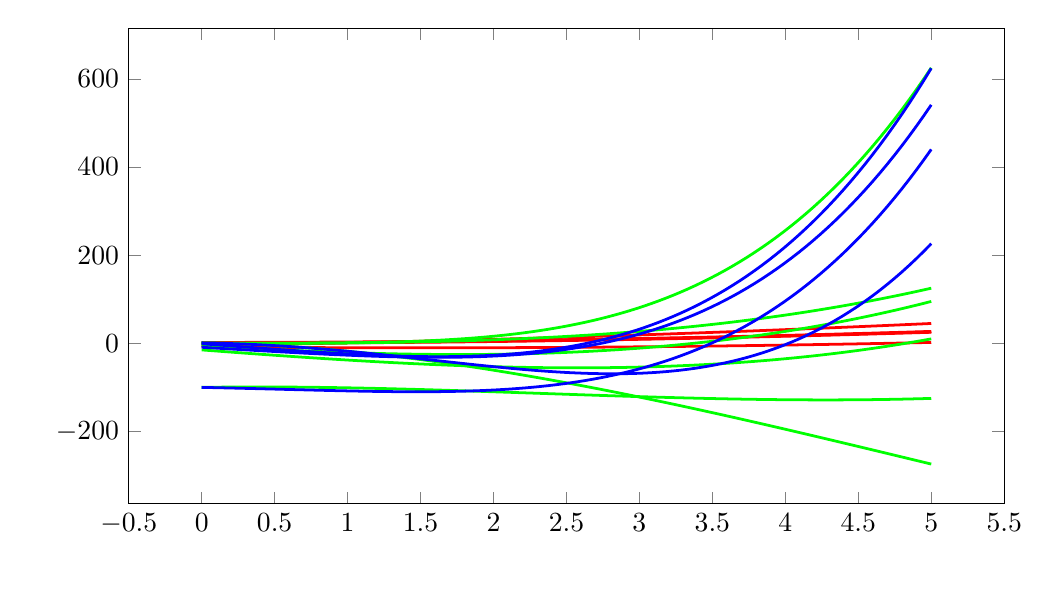
\begin{tikzpicture}[line width=1]
\begin{axis}[width=5in, height=3in,
             scatter/classes={a={mark=*,draw=black}},
             xlabel={\mbox{}},
             xlabel style={name=xlabel}, 
             ylabel={\mbox{}}, 
             legend style={
                at={(xlabel.south)},
                yshift=-1ex,
                anchor=north,
                legend cell align=left,
                },
        ]
]
\addplot[draw=red, line width=1] coordinates {(0.0,0.0)
(0.0505,0.0026)
(0.101,0.0102)
(0.1515,0.023)
(0.202,0.0408)
(0.2525,0.0638)
(0.303,0.0918)
(0.3535,0.125)
(0.404,0.1632)
(0.4545,0.2066)
(0.5051,0.2551)
(0.5556,0.3086)
(0.6061,0.3673)
(0.6566,0.4311)
(0.7071,0.4999)
(0.7576,0.5739)
(0.8081,0.653)
(0.8586,0.7372)
(0.9091,0.8264)
(0.9596,0.9208)
(1.0101,1.0203)
(1.0606,1.1249)
(1.1111,1.2346)
(1.1616,1.3494)
(1.2121,1.4692)
(1.2626,1.5942)
(1.3131,1.7243)
(1.3636,1.8595)
(1.4141,1.9998)
(1.4646,2.1452)
(1.5152,2.2957)
(1.5657,2.4513)
(1.6162,2.612)
(1.6667,2.7778)
(1.7172,2.9487)
(1.7677,3.1247)
(1.8182,3.3058)
(1.8687,3.492)
(1.9192,3.6833)
(1.9697,3.8797)
(2.0202,4.0812)
(2.0707,4.2878)
(2.1212,4.4995)
(2.1717,4.7164)
(2.2222,4.9383)
(2.2727,5.1653)
(2.3232,5.3974)
(2.3737,5.6346)
(2.4242,5.877)
(2.4747,6.1244)
(2.5253,6.3769)
(2.5758,6.6345)
(2.6263,6.8973)
(2.6768,7.1651)
(2.7273,7.438)
(2.7778,7.716)
(2.8283,7.9992)
(2.8788,8.2874)
(2.9293,8.5808)
(2.9798,8.8792)
(3.0303,9.1827)
(3.0808,9.4914)
(3.1313,9.8051)
(3.1818,10.124)
(3.2323,10.4479)
(3.2828,10.777)
(3.3333,11.1111)
(3.3838,11.4504)
(3.4343,11.7947)
(3.4848,12.1442)
(3.5354,12.4987)
(3.5859,12.8584)
(3.6364,13.2231)
(3.6869,13.593)
(3.7374,13.968)
(3.7879,14.348)
(3.8384,14.7332)
(3.8889,15.1235)
(3.9394,15.5188)
(3.9899,15.9193)
(4.0404,16.3249)
(4.0909,16.7355)
(4.1414,17.1513)
(4.1919,17.5722)
(4.2424,17.9982)
(4.2929,18.4292)
(4.3434,18.8654)
(4.3939,19.3067)
(4.4444,19.7531)
(4.4949,20.2046)
(4.5455,20.6612)
(4.596,21.1228)
(4.6465,21.5896)
(4.697,22.0615)
(4.7475,22.5385)
(4.798,23.0206)
(4.8485,23.5078)
(4.899,24.0001)
(4.9495,24.4975)
(5.0,25.0)
(5.0,25.0)};\addplot[draw=red, line width=1] coordinates {(0.0,2.0)
(0.0505,2.0026)
(0.101,2.0102)
(0.1515,2.023)
(0.202,2.0408)
(0.2525,2.0638)
(0.303,2.0918)
(0.3535,2.125)
(0.404,2.1632)
(0.4545,2.2066)
(0.5051,2.2551)
(0.5556,2.3086)
(0.6061,2.3673)
(0.6566,2.4311)
(0.7071,2.4999)
(0.7576,2.5739)
(0.8081,2.653)
(0.8586,2.7372)
(0.9091,2.8264)
(0.9596,2.9208)
(1.0101,3.0203)
(1.0606,3.1249)
(1.1111,3.2346)
(1.1616,3.3494)
(1.2121,3.4692)
(1.2626,3.5942)
(1.3131,3.7243)
(1.3636,3.8595)
(1.4141,3.9998)
(1.4646,4.1452)
(1.5152,4.2957)
(1.5657,4.4513)
(1.6162,4.612)
(1.6667,4.7778)
(1.7172,4.9487)
(1.7677,5.1247)
(1.8182,5.3058)
(1.8687,5.492)
(1.9192,5.6833)
(1.9697,5.8797)
(2.0202,6.0812)
(2.0707,6.2878)
(2.1212,6.4995)
(2.1717,6.7164)
(2.2222,6.9383)
(2.2727,7.1653)
(2.3232,7.3974)
(2.3737,7.6346)
(2.4242,7.877)
(2.4747,8.1244)
(2.5253,8.3769)
(2.5758,8.6345)
(2.6263,8.8973)
(2.6768,9.1651)
(2.7273,9.438)
(2.7778,9.716)
(2.8283,9.9992)
(2.8788,10.2874)
(2.9293,10.5808)
(2.9798,10.8792)
(3.0303,11.1827)
(3.0808,11.4914)
(3.1313,11.8051)
(3.1818,12.124)
(3.2323,12.4479)
(3.2828,12.777)
(3.3333,13.1111)
(3.3838,13.4504)
(3.4343,13.7947)
(3.4848,14.1442)
(3.5354,14.4987)
(3.5859,14.8584)
(3.6364,15.2231)
(3.6869,15.593)
(3.7374,15.968)
(3.7879,16.348)
(3.8384,16.7332)
(3.8889,17.1235)
(3.9394,17.5188)
(3.9899,17.9193)
(4.0404,18.3249)
(4.0909,18.7355)
(4.1414,19.1513)
(4.1919,19.5722)
(4.2424,19.9982)
(4.2929,20.4292)
(4.3434,20.8654)
(4.3939,21.3067)
(4.4444,21.7531)
(4.4949,22.2046)
(4.5455,22.6612)
(4.596,23.1228)
(4.6465,23.5896)
(4.697,24.0615)
(4.7475,24.5385)
(4.798,25.0206)
(4.8485,25.5078)
(4.899,26.0001)
(4.9495,26.4975)
(5.0,27.0)
(5.0,27.0)};\addplot[draw=red, line width=1] coordinates {(0.0,1.0)
(0.0505,1.0026)
(0.101,1.0102)
(0.1515,1.023)
(0.202,1.0408)
(0.2525,1.0638)
(0.303,1.0918)
(0.3535,1.125)
(0.404,1.1632)
(0.4545,1.2066)
(0.5051,1.2551)
(0.5556,1.3086)
(0.6061,1.3673)
(0.6566,1.4311)
(0.7071,1.4999)
(0.7576,1.5739)
(0.8081,1.653)
(0.8586,1.7372)
(0.9091,1.8264)
(0.9596,1.9208)
(1.0101,2.0203)
(1.0606,2.1249)
(1.1111,2.2346)
(1.1616,2.3494)
(1.2121,2.4692)
(1.2626,2.5942)
(1.3131,2.7243)
(1.3636,2.8595)
(1.4141,2.9998)
(1.4646,3.1452)
(1.5152,3.2957)
(1.5657,3.4513)
(1.6162,3.612)
(1.6667,3.7778)
(1.7172,3.9487)
(1.7677,4.1247)
(1.8182,4.3058)
(1.8687,4.492)
(1.9192,4.6833)
(1.9697,4.8797)
(2.0202,5.0812)
(2.0707,5.2878)
(2.1212,5.4995)
(2.1717,5.7164)
(2.2222,5.9383)
(2.2727,6.1653)
(2.3232,6.3974)
(2.3737,6.6346)
(2.4242,6.877)
(2.4747,7.1244)
(2.5253,7.3769)
(2.5758,7.6345)
(2.6263,7.8973)
(2.6768,8.1651)
(2.7273,8.438)
(2.7778,8.716)
(2.8283,8.9992)
(2.8788,9.2874)
(2.9293,9.5808)
(2.9798,9.8792)
(3.0303,10.1827)
(3.0808,10.4914)
(3.1313,10.8051)
(3.1818,11.124)
(3.2323,11.4479)
(3.2828,11.777)
(3.3333,12.1111)
(3.3838,12.4504)
(3.4343,12.7947)
(3.4848,13.1442)
(3.5354,13.4987)
(3.5859,13.8584)
(3.6364,14.2231)
(3.6869,14.593)
(3.7374,14.968)
(3.7879,15.348)
(3.8384,15.7332)
(3.8889,16.1235)
(3.9394,16.5188)
(3.9899,16.9193)
(4.0404,17.3249)
(4.0909,17.7355)
(4.1414,18.1513)
(4.1919,18.5722)
(4.2424,18.9982)
(4.2929,19.4292)
(4.3434,19.8654)
(4.3939,20.3067)
(4.4444,20.7531)
(4.4949,21.2046)
(4.5455,21.6612)
(4.596,22.1228)
(4.6465,22.5896)
(4.697,23.0615)
(4.7475,23.5385)
(4.798,24.0206)
(4.8485,24.5078)
(4.899,25.0001)
(4.9495,25.4975)
(5.0,26.0)
(5.0,26.0)};\addplot[draw=red, line width=1] coordinates {(0.0,-5.0)
(0.0505,-4.7449)
(0.101,-4.4847)
(0.1515,-4.2195)
(0.202,-3.9491)
(0.2525,-3.6736)
(0.303,-3.393)
(0.3535,-3.1073)
(0.404,-2.8165)
(0.4545,-2.5207)
(0.5051,-2.2197)
(0.5556,-1.9136)
(0.6061,-1.6024)
(0.6566,-1.2861)
(0.7071,-0.9647)
(0.7576,-0.6382)
(0.8081,-0.3066)
(0.8586,0.0301)
(0.9091,0.3719)
(0.9596,0.7188)
(1.0101,1.0708)
(1.0606,1.4279)
(1.1111,1.7901)
(1.1616,2.1574)
(1.2121,2.5298)
(1.2626,2.9074)
(1.3131,3.29)
(1.3636,3.6777)
(1.4141,4.0705)
(1.4646,4.4684)
(1.5152,4.8714)
(1.5657,5.2796)
(1.6162,5.6928)
(1.6667,6.1111)
(1.7172,6.5345)
(1.7677,6.9631)
(1.8182,7.3967)
(1.8687,7.8354)
(1.9192,8.2793)
(1.9697,8.7282)
(2.0202,9.1822)
(2.0707,9.6414)
(2.1212,10.1056)
(2.1717,10.5749)
(2.2222,11.0494)
(2.2727,11.5289)
(2.3232,12.0136)
(2.3737,12.5033)
(2.4242,12.9982)
(2.4747,13.4981)
(2.5253,14.0032)
(2.5758,14.5133)
(2.6263,15.0286)
(2.6768,15.5489)
(2.7273,16.0744)
(2.7778,16.6049)
(2.8283,17.1406)
(2.8788,17.6814)
(2.9293,18.2272)
(2.9798,18.7782)
(3.0303,19.3343)
(3.0808,19.8954)
(3.1313,20.4617)
(3.1818,21.0331)
(3.2323,21.6095)
(3.2828,22.1911)
(3.3333,22.7778)
(3.3838,23.3696)
(3.4343,23.9664)
(3.4848,24.5684)
(3.5354,25.1755)
(3.5859,25.7877)
(3.6364,26.405)
(3.6869,27.0273)
(3.7374,27.6548)
(3.7879,28.2874)
(3.8384,28.9251)
(3.8889,29.5679)
(3.9394,30.2158)
(3.9899,30.8688)
(4.0404,31.5269)
(4.0909,32.1901)
(4.1414,32.8584)
(4.1919,33.5318)
(4.2424,34.2103)
(4.2929,34.8939)
(4.3434,35.5826)
(4.3939,36.2764)
(4.4444,36.9753)
(4.4949,37.6793)
(4.5455,38.3884)
(4.596,39.1026)
(4.6465,39.822)
(4.697,40.5464)
(4.7475,41.2759)
(4.798,42.0105)
(4.8485,42.7502)
(4.899,43.4951)
(4.9495,44.245)
(5.0,45.0)
(5.0,45.0)};\addplot[draw=red, line width=1] coordinates {(0.0,-8.0)
(0.0505,-8.149)
(0.101,-8.2928)
(0.1515,-8.4316)
(0.202,-8.5652)
(0.2525,-8.6938)
(0.303,-8.8173)
(0.3535,-8.9356)
(0.404,-9.0489)
(0.4545,-9.157)
(0.5051,-9.2601)
(0.5556,-9.358)
(0.6061,-9.4509)
(0.6566,-9.5386)
(0.7071,-9.6213)
(0.7576,-9.6988)
(0.8081,-9.7712)
(0.8586,-9.8386)
(0.9091,-9.9008)
(0.9596,-9.958)
(1.0101,-10.01)
(1.0606,-10.0569)
(1.1111,-10.0988)
(1.1616,-10.1355)
(1.2121,-10.1671)
(1.2626,-10.1937)
(1.3131,-10.2151)
(1.3636,-10.2314)
(1.4141,-10.2426)
(1.4646,-10.2488)
(1.5152,-10.2498)
(1.5657,-10.2457)
(1.6162,-10.2365)
(1.6667,-10.2222)
(1.7172,-10.2028)
(1.7677,-10.1783)
(1.8182,-10.1488)
(1.8687,-10.1141)
(1.9192,-10.0743)
(1.9697,-10.0294)
(2.0202,-9.9794)
(2.0707,-9.9243)
(2.1212,-9.8641)
(2.1717,-9.7988)
(2.2222,-9.7284)
(2.2727,-9.6529)
(2.3232,-9.5723)
(2.3737,-9.4866)
(2.4242,-9.3958)
(2.4747,-9.2999)
(2.5253,-9.1989)
(2.5758,-9.0927)
(2.6263,-8.9815)
(2.6768,-8.8652)
(2.7273,-8.7438)
(2.7778,-8.6173)
(2.8283,-8.4857)
(2.8788,-8.3489)
(2.9293,-8.2071)
(2.9798,-8.0602)
(3.0303,-7.9082)
(3.0808,-7.751)
(3.1313,-7.5888)
(3.1818,-7.4215)
(3.2323,-7.2491)
(3.2828,-7.0715)
(3.3333,-6.8889)
(3.3838,-6.7012)
(3.4343,-6.5083)
(3.4848,-6.3104)
(3.5354,-6.1073)
(3.5859,-5.8992)
(3.6364,-5.686)
(3.6869,-5.4676)
(3.7374,-5.2442)
(3.7879,-5.0156)
(3.8384,-4.782)
(3.8889,-4.5432)
(3.9394,-4.2994)
(3.9899,-4.0504)
(4.0404,-3.7963)
(4.0909,-3.5372)
(4.1414,-3.2729)
(4.1919,-3.0036)
(4.2424,-2.7291)
(4.2929,-2.4495)
(4.3434,-2.1649)
(4.3939,-1.8751)
(4.4444,-1.5802)
(4.4949,-1.2803)
(4.5455,-0.9752)
(4.596,-0.665)
(4.6465,-0.3498)
(4.697,-0.0294)
(4.7475,0.2961)
(4.798,0.6267)
(4.8485,0.9624)
(4.899,1.3031)
(4.9495,1.649)
(5.0,2.0)
(5.0,2.0)};\addplot[draw=green, line width=1] coordinates {(0.0,0.0)
(0.0505,0.0001)
(0.101,0.001)
(0.1515,0.0035)
(0.202,0.0082)
(0.2525,0.0161)
(0.303,0.0278)
(0.3535,0.0442)
(0.404,0.066)
(0.4545,0.0939)
(0.5051,0.1288)
(0.5556,0.1715)
(0.6061,0.2226)
(0.6566,0.283)
(0.7071,0.3535)
(0.7576,0.4348)
(0.8081,0.5277)
(0.8586,0.6329)
(0.9091,0.7513)
(0.9596,0.8836)
(1.0101,1.0306)
(1.0606,1.1931)
(1.1111,1.3717)
(1.1616,1.5674)
(1.2121,1.7809)
(1.2626,2.0129)
(1.3131,2.2643)
(1.3636,2.5357)
(1.4141,2.828)
(1.4646,3.1419)
(1.5152,3.4783)
(1.5657,3.8379)
(1.6162,4.2214)
(1.6667,4.6296)
(1.7172,5.0634)
(1.7677,5.5234)
(1.8182,6.0105)
(1.8687,6.5254)
(1.9192,7.069)
(1.9697,7.6418)
(2.0202,8.2449)
(2.0707,8.8788)
(2.1212,9.5445)
(2.1717,10.2426)
(2.2222,10.9739)
(2.2727,11.7393)
(2.3232,12.5394)
(2.3737,13.3751)
(2.4242,14.2472)
(2.4747,15.1563)
(2.5253,16.1033)
(2.5758,17.0889)
(2.6263,18.114)
(2.6768,19.1793)
(2.7273,20.2855)
(2.7778,21.4335)
(2.8283,22.624)
(2.8788,23.8577)
(2.9293,25.1356)
(2.9798,26.4582)
(3.0303,27.8265)
(3.0808,29.2411)
(3.1313,30.7029)
(3.1818,32.2126)
(3.2323,33.771)
(3.2828,35.3789)
(3.3333,37.037)
(3.3838,38.7462)
(3.4343,40.5071)
(3.4848,42.3206)
(3.5354,44.1874)
(3.5859,46.1083)
(3.6364,48.0841)
(3.6869,50.1156)
(3.7374,52.2035)
(3.7879,54.3486)
(3.8384,56.5516)
(3.8889,58.8134)
(3.9394,61.1348)
(3.9899,63.5164)
(4.0404,65.959)
(4.0909,68.4636)
(4.1414,71.0307)
(4.1919,73.6612)
(4.2424,76.3558)
(4.2929,79.1154)
(4.3434,81.9407)
(4.3939,84.8325)
(4.4444,87.7915)
(4.4949,90.8185)
(4.5455,93.9144)
(4.596,97.0797)
(4.6465,100.3155)
(4.697,103.6223)
(4.7475,107.001)
(4.798,110.4524)
(4.8485,113.9772)
(4.899,117.5763)
(4.9495,121.2503)
(5.0,125.0)
(5.0,125.0)};\addplot[draw=green, line width=1] coordinates {(0.0,-5.0)
(0.0505,-6.0023)
(0.101,-6.9886)
(0.1515,-7.958)
(0.202,-8.9097)
(0.2525,-9.8431)
(0.303,-10.7573)
(0.3535,-11.6516)
(0.404,-12.5251)
(0.4545,-13.3772)
(0.5051,-14.207)
(0.5556,-15.0137)
(0.6061,-15.7967)
(0.6566,-16.555)
(0.7071,-17.2881)
(0.7576,-17.995)
(0.8081,-18.675)
(0.8586,-19.3273)
(0.9091,-19.9512)
(0.9596,-20.5458)
(1.0101,-21.1105)
(1.0606,-21.6444)
(1.1111,-22.1468)
(1.1616,-22.6168)
(1.2121,-23.0538)
(1.2626,-23.4569)
(1.3131,-23.8254)
(1.3636,-24.1585)
(1.4141,-24.4554)
(1.4646,-24.7154)
(1.5152,-24.9377)
(1.5657,-25.1214)
(1.6162,-25.2659)
(1.6667,-25.3704)
(1.7172,-25.434)
(1.7677,-25.4561)
(1.8182,-25.4358)
(1.8687,-25.3723)
(1.9192,-25.265)
(1.9697,-25.113)
(2.0202,-24.9155)
(2.0707,-24.6718)
(2.1212,-24.3811)
(2.1717,-24.0427)
(2.2222,-23.6557)
(2.2727,-23.2194)
(2.3232,-22.733)
(2.3737,-22.1957)
(2.4242,-21.6068)
(2.4747,-20.9655)
(2.5253,-20.2711)
(2.5758,-19.5226)
(2.6263,-18.7195)
(2.6768,-17.8608)
(2.7273,-16.9459)
(2.7778,-15.9739)
(2.8283,-14.9442)
(2.8788,-13.8558)
(2.9293,-12.708)
(2.9798,-11.5002)
(3.0303,-10.2314)
(3.0808,-8.9009)
(3.1313,-7.508)
(3.1818,-6.0518)
(3.2323,-4.5317)
(3.2828,-2.9468)
(3.3333,-1.2963)
(3.3838,0.4205)
(3.4343,2.2044)
(3.4848,4.0561)
(3.5354,5.9765)
(3.5859,7.9663)
(3.6364,10.0263)
(3.6869,12.1572)
(3.7374,14.3599)
(3.7879,16.6351)
(3.8384,18.9835)
(3.8889,21.406)
(3.9394,23.9034)
(3.9899,26.4763)
(4.0404,29.1256)
(4.0909,31.852)
(4.1414,34.6563)
(4.1919,37.5394)
(4.2424,40.5019)
(4.2929,43.5446)
(4.3434,46.6683)
(4.3939,49.8738)
(4.4444,53.1619)
(4.4949,56.5332)
(4.5455,59.9887)
(4.596,63.5291)
(4.6465,67.1551)
(4.697,70.8675)
(4.7475,74.6671)
(4.798,78.5547)
(4.8485,82.531)
(4.899,86.5968)
(4.9495,90.7529)
(5.0,95.0)
(5.0,95.0)};\addplot[draw=green, line width=1] coordinates {(0.0,-15.0)
(0.0505,-16.2599)
(0.101,-17.514)
(0.1515,-18.7614)
(0.202,-20.0014)
(0.2525,-21.2333)
(0.303,-22.4561)
(0.3535,-23.6692)
(0.404,-24.8718)
(0.4545,-26.0631)
(0.5051,-27.2424)
(0.5556,-28.4088)
(0.6061,-29.5616)
(0.6566,-30.7)
(0.7071,-31.8233)
(0.7576,-32.9307)
(0.8081,-34.0214)
(0.8586,-35.0946)
(0.9091,-36.1495)
(0.9596,-37.1855)
(1.0101,-38.2016)
(1.0606,-39.1972)
(1.1111,-40.1715)
(1.1616,-41.1236)
(1.2121,-42.0529)
(1.2626,-42.9585)
(1.3131,-43.8397)
(1.3636,-44.6957)
(1.4141,-45.5257)
(1.4646,-46.329)
(1.5152,-47.1048)
(1.5657,-47.8523)
(1.6162,-48.5707)
(1.6667,-49.2593)
(1.7172,-49.9172)
(1.7677,-50.5438)
(1.8182,-51.1382)
(1.8687,-51.6997)
(1.9192,-52.2275)
(1.9697,-52.7209)
(2.0202,-53.179)
(2.0707,-53.601)
(2.1212,-53.9863)
(2.1717,-54.334)
(2.2222,-54.6433)
(2.2727,-54.9136)
(2.3232,-55.144)
(2.3737,-55.3337)
(2.4242,-55.482)
(2.4747,-55.588)
(2.5253,-55.6511)
(2.5758,-55.6705)
(2.6263,-55.6453)
(2.6768,-55.5748)
(2.7273,-55.4583)
(2.7778,-55.2949)
(2.8283,-55.0839)
(2.8788,-54.8246)
(2.9293,-54.516)
(2.9798,-54.1575)
(3.0303,-53.7484)
(3.0808,-53.2877)
(3.1313,-52.7748)
(3.1818,-52.2089)
(3.2323,-51.5891)
(3.2828,-50.9148)
(3.3333,-50.1852)
(3.3838,-49.3994)
(3.4343,-48.5568)
(3.4848,-47.6565)
(3.5354,-46.6977)
(3.5859,-45.6797)
(3.6364,-44.6018)
(3.6869,-43.4631)
(3.7374,-42.2629)
(3.7879,-41.0004)
(3.8384,-39.6748)
(3.8889,-38.2853)
(3.9394,-36.8313)
(3.9899,-35.3118)
(4.0404,-33.7262)
(4.0909,-32.0736)
(4.1414,-30.3534)
(4.1919,-28.5646)
(4.2424,-26.7066)
(4.2929,-24.7786)
(4.3434,-22.7797)
(4.3939,-20.7093)
(4.4444,-18.5665)
(4.4949,-16.3506)
(4.5455,-14.0609)
(4.596,-11.6964)
(4.6465,-9.2565)
(4.697,-6.7404)
(4.7475,-4.1473)
(4.798,-1.4765)
(4.8485,1.2729)
(4.899,4.1016)
(4.9495,7.0104)
(5.0,10.0)
(5.0,10.0)};\addplot[draw=green, line width=1] coordinates {(0.0,1.0)
(0.0505,0.7093)
(0.101,0.3429)
(0.1515,-0.0985)
(0.202,-0.614)
(0.2525,-1.2031)
(0.303,-1.8647)
(0.3535,-2.5983)
(0.404,-3.403)
(0.4545,-4.278)
(0.5051,-5.2226)
(0.5556,-6.2359)
(0.6061,-7.3173)
(0.6566,-8.466)
(0.7071,-9.6811)
(0.7576,-10.9619)
(0.8081,-12.3077)
(0.8586,-13.7176)
(0.9091,-15.1908)
(0.9596,-16.7267)
(1.0101,-18.3245)
(1.0606,-19.9832)
(1.1111,-21.7023)
(1.1616,-23.4809)
(1.2121,-25.3183)
(1.2626,-27.2136)
(1.3131,-29.1661)
(1.3636,-31.1751)
(1.4141,-33.2397)
(1.4646,-35.3591)
(1.5152,-37.5327)
(1.5657,-39.7596)
(1.6162,-42.0391)
(1.6667,-44.3704)
(1.7172,-46.7527)
(1.7677,-49.1852)
(1.8182,-51.6672)
(1.8687,-54.1979)
(1.9192,-56.7765)
(1.9697,-59.4022)
(2.0202,-62.0744)
(2.0707,-64.7921)
(2.1212,-67.5547)
(2.1717,-70.3613)
(2.2222,-73.2112)
(2.2727,-76.1037)
(2.3232,-79.0379)
(2.3737,-82.013)
(2.4242,-85.0283)
(2.4747,-88.0831)
(2.5253,-91.1765)
(2.5758,-94.3078)
(2.6263,-97.4761)
(2.6768,-100.6808)
(2.7273,-103.9211)
(2.7778,-107.1962)
(2.8283,-110.5052)
(2.8788,-113.8475)
(2.9293,-117.2223)
(2.9798,-120.6287)
(3.0303,-124.0661)
(3.0808,-127.5336)
(3.1313,-131.0305)
(3.1818,-134.556)
(3.2323,-138.1093)
(3.2828,-141.6897)
(3.3333,-145.2963)
(3.3838,-148.9284)
(3.4343,-152.5853)
(3.4848,-156.2662)
(3.5354,-159.9702)
(3.5859,-163.6967)
(3.6364,-167.4448)
(3.6869,-171.2137)
(3.7374,-175.0028)
(3.7879,-178.8112)
(3.8384,-182.6381)
(3.8889,-186.4829)
(3.9394,-190.3446)
(3.9899,-194.2225)
(4.0404,-198.1159)
(4.0909,-202.024)
(4.1414,-205.9461)
(4.1919,-209.8812)
(4.2424,-213.8287)
(4.2929,-217.7878)
(4.3434,-221.7578)
(4.3939,-225.7378)
(4.4444,-229.727)
(4.4949,-233.7248)
(4.5455,-237.7303)
(4.596,-241.7427)
(4.6465,-245.7614)
(4.697,-249.7854)
(4.7475,-253.8141)
(4.798,-257.8466)
(4.8485,-261.8823)
(4.899,-265.9202)
(4.9495,-269.9597)
(5.0,-274.0)
(5.0,-274.0)};\addplot[draw=green, line width=1] coordinates {(0.0,-100.0)
(0.0505,-99.7652)
(0.101,-99.5653)
(0.1515,-99.3996)
(0.202,-99.2673)
(0.2525,-99.1677)
(0.303,-99.0998)
(0.3535,-99.063)
(0.404,-99.0566)
(0.4545,-99.0796)
(0.5051,-99.1315)
(0.5556,-99.2112)
(0.6061,-99.3183)
(0.6566,-99.4517)
(0.7071,-99.6108)
(0.7576,-99.7948)
(0.8081,-100.0029)
(0.8586,-100.2343)
(0.9091,-100.4884)
(0.9596,-100.7642)
(1.0101,-101.061)
(1.0606,-101.3781)
(1.1111,-101.7147)
(1.1616,-102.07)
(1.2121,-102.4432)
(1.2626,-102.8335)
(1.3131,-103.2403)
(1.3636,-103.6627)
(1.4141,-104.0999)
(1.4646,-104.5511)
(1.5152,-105.0157)
(1.5657,-105.4928)
(1.6162,-105.9817)
(1.6667,-106.4815)
(1.7172,-106.9915)
(1.7677,-107.511)
(1.8182,-108.0391)
(1.8687,-108.5751)
(1.9192,-109.1182)
(1.9697,-109.6676)
(2.0202,-110.2226)
(2.0707,-110.7824)
(2.1212,-111.3462)
(2.1717,-111.9133)
(2.2222,-112.4829)
(2.2727,-113.0541)
(2.3232,-113.6263)
(2.3737,-114.1986)
(2.4242,-114.7703)
(2.4747,-115.3406)
(2.5253,-115.9088)
(2.5758,-116.474)
(2.6263,-117.0355)
(2.6768,-117.5925)
(2.7273,-118.1443)
(2.7778,-118.69)
(2.8283,-119.2289)
(2.8788,-119.7603)
(2.9293,-120.2833)
(2.9798,-120.7972)
(3.0303,-121.3012)
(3.0808,-121.7945)
(3.1313,-122.2764)
(3.1818,-122.7461)
(3.2323,-123.2027)
(3.2828,-123.6457)
(3.3333,-124.0741)
(3.3838,-124.4872)
(3.4343,-124.8842)
(3.4848,-125.2644)
(3.5354,-125.6269)
(3.5859,-125.971)
(3.6364,-126.296)
(3.6869,-126.6011)
(3.7374,-126.8854)
(3.7879,-127.1482)
(3.8384,-127.3888)
(3.8889,-127.6063)
(3.9394,-127.8)
(3.9899,-127.9692)
(4.0404,-128.113)
(4.0909,-128.2307)
(4.1414,-128.3214)
(4.1919,-128.3845)
(4.2424,-128.4192)
(4.2929,-128.4246)
(4.3434,-128.4001)
(4.3939,-128.3447)
(4.4444,-128.2579)
(4.4949,-128.1387)
(4.5455,-127.9865)
(4.596,-127.8004)
(4.6465,-127.5796)
(4.697,-127.3235)
(4.7475,-127.0312)
(4.798,-126.7019)
(4.8485,-126.335)
(4.899,-125.9295)
(4.9495,-125.4848)
(5.0,-125.0)
(5.0,-125.0)};\addplot[draw=green, line width=1] coordinates {(0.0,0.0)
(0.0505,0.0)
(0.101,0.0001)
(0.1515,0.0005)
(0.202,0.0017)
(0.2525,0.0041)
(0.303,0.0084)
(0.3535,0.0156)
(0.404,0.0267)
(0.4545,0.0427)
(0.5051,0.0651)
(0.5556,0.0953)
(0.6061,0.1349)
(0.6566,0.1858)
(0.7071,0.2499)
(0.7576,0.3294)
(0.8081,0.4264)
(0.8586,0.5434)
(0.9091,0.683)
(0.9596,0.8479)
(1.0101,1.041)
(1.0606,1.2654)
(1.1111,1.5242)
(1.1616,1.8208)
(1.2121,2.1587)
(1.2626,2.5416)
(1.3131,2.9733)
(1.3636,3.4578)
(1.4141,3.9992)
(1.4646,4.6018)
(1.5152,5.2702)
(1.5657,6.0088)
(1.6162,6.8224)
(1.6667,7.716)
(1.7172,8.6947)
(1.7677,9.7636)
(1.8182,10.9282)
(1.8687,12.194)
(1.9192,13.5667)
(1.9697,15.0521)
(2.0202,16.6563)
(2.0707,18.3855)
(2.1212,20.2459)
(2.1717,22.244)
(2.2222,24.3865)
(2.2727,26.6802)
(2.3232,29.132)
(2.3737,31.749)
(2.4242,34.5386)
(2.4747,37.508)
(2.5253,40.6649)
(2.5758,44.0169)
(2.6263,47.5721)
(2.6768,51.3384)
(2.7273,55.3241)
(2.7778,59.5374)
(2.8283,63.9869)
(2.8788,68.6813)
(2.9293,73.6294)
(2.9798,78.8401)
(3.0303,84.3226)
(3.0808,90.0863)
(3.1313,96.1404)
(3.1818,102.4947)
(3.2323,109.1589)
(3.2828,116.1429)
(3.3333,123.4568)
(3.3838,131.1108)
(3.4343,139.1153)
(3.4848,147.4808)
(3.5354,156.2181)
(3.5859,165.338)
(3.6364,174.8514)
(3.6869,184.7697)
(3.7374,195.104)
(3.7879,205.8658)
(3.8384,217.0669)
(3.8889,228.7189)
(3.9394,240.8339)
(3.9899,253.4239)
(4.0404,266.5012)
(4.0909,280.0782)
(4.1414,294.1675)
(4.1919,308.7817)
(4.2424,323.9339)
(4.2929,339.637)
(4.3434,355.9041)
(4.3939,372.7488)
(4.4444,390.1844)
(4.4949,408.2247)
(4.5455,426.8834)
(4.596,446.1746)
(4.6465,466.1123)
(4.697,486.7109)
(4.7475,507.9847)
(4.798,529.9485)
(4.8485,552.6169)
(4.899,576.0049)
(4.9495,600.1275)
(5.0,625.0)
(5.0,625.0)};\addplot[draw=blue, line width=1] coordinates {(0.0,-9.0)
(0.0505,-10.0075)
(0.101,-11.0099)
(0.1515,-12.0068)
(0.202,-12.9979)
(0.2525,-13.9827)
(0.303,-14.9603)
(0.3535,-15.9301)
(0.404,-16.8909)
(0.4545,-17.8416)
(0.5051,-18.7809)
(0.5556,-19.7072)
(0.6061,-20.619)
(0.6566,-21.5144)
(0.7071,-22.3915)
(0.7576,-23.2482)
(0.8081,-24.0822)
(0.8586,-24.8911)
(0.9091,-25.6724)
(0.9596,-26.4232)
(1.0101,-27.1407)
(1.0606,-27.8219)
(1.1111,-28.4635)
(1.1616,-29.0622)
(1.2121,-29.6145)
(1.2626,-30.1167)
(1.3131,-30.5651)
(1.3636,-30.9555)
(1.4141,-31.2838)
(1.4646,-31.5459)
(1.5152,-31.7372)
(1.5657,-31.8531)
(1.6162,-31.8888)
(1.6667,-31.8395)
(1.7172,-31.7)
(1.7677,-31.4652)
(1.8182,-31.1296)
(1.8687,-30.6877)
(1.9192,-30.1339)
(1.9697,-29.4621)
(2.0202,-28.6665)
(2.0707,-27.7408)
(2.1212,-26.6788)
(2.1717,-25.474)
(2.2222,-24.1196)
(2.2727,-22.609)
(2.3232,-20.9352)
(2.3737,-19.0911)
(2.4242,-17.0693)
(2.4747,-14.8626)
(2.5253,-12.4633)
(2.5758,-9.8637)
(2.6263,-7.0559)
(2.6768,-4.0318)
(2.7273,-0.7833)
(2.7778,2.6979)
(2.8283,6.4205)
(2.8788,10.393)
(2.9293,14.6243)
(2.9798,19.1234)
(3.0303,23.8993)
(3.0808,28.9615)
(3.1313,34.3193)
(3.1818,39.9823)
(3.2323,45.9603)
(3.2828,52.2633)
(3.3333,58.9012)
(3.3838,65.8844)
(3.4343,73.2231)
(3.4848,80.928)
(3.5354,89.0098)
(3.5859,97.4792)
(3.6364,106.3473)
(3.6869,115.6253)
(3.7374,125.3245)
(3.7879,135.4563)
(3.8384,146.0324)
(3.8889,157.0646)
(3.9394,168.5649)
(3.9899,180.5452)
(4.0404,193.018)
(4.0909,205.9956)
(4.1414,219.4905)
(4.1919,233.5155)
(4.2424,248.0836)
(4.2929,263.2076)
(4.3434,278.9009)
(4.3939,295.1767)
(4.4444,312.0486)
(4.4949,329.5303)
(4.5455,347.6355)
(4.596,366.3782)
(4.6465,385.7726)
(4.697,405.833)
(4.7475,426.5737)
(4.798,448.0095)
(4.8485,470.155)
(4.899,493.0252)
(4.9495,516.6351)
(5.0,541.0)
(5.0,541.0)};\addplot[draw=blue, line width=1] coordinates {(0.0,-1.0)
(0.0505,-2.2625)
(0.101,-3.5241)
(0.1515,-4.7839)
(0.202,-6.0406)
(0.2525,-7.293)
(0.303,-8.5395)
(0.3535,-9.7786)
(0.404,-11.0084)
(0.4545,-12.227)
(0.5051,-13.4324)
(0.5556,-14.6222)
(0.6061,-15.794)
(0.6566,-16.9453)
(0.7071,-18.0733)
(0.7576,-19.1752)
(0.8081,-20.2479)
(0.8586,-21.2883)
(0.9091,-22.2929)
(0.9596,-23.2584)
(1.0101,-24.1809)
(1.0606,-25.0567)
(1.1111,-25.8819)
(1.1616,-26.6522)
(1.2121,-27.3635)
(1.2626,-28.0112)
(1.3131,-28.5908)
(1.3636,-29.0975)
(1.4141,-29.5264)
(1.4646,-29.8724)
(1.5152,-30.1303)
(1.5657,-30.2948)
(1.6162,-30.3602)
(1.6667,-30.321)
(1.7172,-30.1712)
(1.7677,-29.9049)
(1.8182,-29.5158)
(1.8687,-28.9977)
(1.9192,-28.3442)
(1.9697,-27.5485)
(2.0202,-26.6038)
(2.0707,-25.5034)
(2.1212,-24.24)
(2.1717,-22.8063)
(2.2222,-21.1951)
(2.2727,-19.3987)
(2.3232,-17.4094)
(2.3737,-15.2193)
(2.4242,-12.8203)
(2.4747,-10.2044)
(2.5253,-7.3632)
(2.5758,-4.2881)
(2.6263,-0.9704)
(2.6768,2.5985)
(2.7273,6.4278)
(2.7778,10.5264)
(2.8283,14.9038)
(2.8788,19.5694)
(2.9293,24.5326)
(2.9798,29.8034)
(3.0303,35.3915)
(3.0808,41.3072)
(3.1313,47.5605)
(3.1818,54.1619)
(3.2323,61.1218)
(3.2828,68.4511)
(3.3333,76.1605)
(3.3838,84.261)
(3.4343,92.7638)
(3.4848,101.6802)
(3.5354,111.0217)
(3.5859,120.7999)
(3.6364,131.0265)
(3.6869,141.7136)
(3.7374,152.8731)
(3.7879,164.5175)
(3.8384,176.6589)
(3.8889,189.3102)
(3.9394,202.4838)
(3.9899,216.1928)
(4.0404,230.4502)
(4.0909,245.269)
(4.1414,260.6628)
(4.1919,276.6449)
(4.2424,293.2291)
(4.2929,310.4292)
(4.3434,328.259)
(4.3939,346.7328)
(4.4444,365.8648)
(4.4949,385.6695)
(4.5455,406.1614)
(4.596,427.3553)
(4.6465,449.2661)
(4.697,471.9089)
(4.7475,495.2989)
(4.798,519.4514)
(4.8485,544.382)
(4.899,570.1064)
(4.9495,596.6404)
(5.0,624.0)
(5.0,624.0)};\addplot[draw=blue, line width=1] coordinates {(0.0,1.0)
(0.0505,0.7092)
(0.101,0.342)
(0.1515,-0.1014)
(0.202,-0.6206)
(0.2525,-1.2151)
(0.303,-1.8841)
(0.3535,-2.6269)
(0.404,-3.4423)
(0.4545,-4.3292)
(0.5051,-5.2863)
(0.5556,-6.3121)
(0.6061,-7.405)
(0.6566,-8.5632)
(0.7071,-9.7846)
(0.7576,-11.0673)
(0.8081,-12.4089)
(0.8586,-13.8071)
(0.9091,-15.2591)
(0.9596,-16.7624)
(1.0101,-18.314)
(1.0606,-19.9109)
(1.1111,-21.5499)
(1.1616,-23.2276)
(1.2121,-24.9405)
(1.2626,-26.685)
(1.3131,-28.4571)
(1.3636,-30.253)
(1.4141,-32.0685)
(1.4646,-33.8992)
(1.5152,-35.7409)
(1.5657,-37.5887)
(1.6162,-39.4381)
(1.6667,-41.284)
(1.7172,-43.1213)
(1.7677,-44.945)
(1.8182,-46.7495)
(1.8687,-48.5293)
(1.9192,-50.2787)
(1.9697,-51.992)
(2.0202,-53.6629)
(2.0707,-55.2855)
(2.1212,-56.8533)
(2.1717,-58.3599)
(2.2222,-59.7987)
(2.2727,-61.1628)
(2.3232,-62.4453)
(2.3737,-63.6391)
(2.4242,-64.7369)
(2.4747,-65.7314)
(2.5253,-66.6149)
(2.5758,-67.3797)
(2.6263,-68.018)
(2.6768,-68.5217)
(2.7273,-68.8825)
(2.7778,-69.0922)
(2.8283,-69.1422)
(2.8788,-69.0239)
(2.9293,-68.7284)
(2.9798,-68.2468)
(3.0303,-67.5699)
(3.0808,-66.6885)
(3.1313,-65.593)
(3.1818,-64.2739)
(3.2323,-62.7214)
(3.2828,-60.9257)
(3.3333,-58.8765)
(3.3838,-56.5638)
(3.4343,-53.9771)
(3.4848,-51.1059)
(3.5354,-47.9395)
(3.5859,-44.467)
(3.6364,-40.6775)
(3.6869,-36.5597)
(3.7374,-32.1023)
(3.7879,-27.2939)
(3.8384,-22.1229)
(3.8889,-16.5774)
(3.9394,-10.6454)
(3.9899,-4.315)
(4.0404,2.4262)
(4.0909,9.5906)
(4.1414,17.1907)
(4.1919,25.2393)
(4.2424,33.7493)
(4.2929,42.7337)
(4.3434,52.2056)
(4.3939,62.1785)
(4.4444,72.6659)
(4.4949,83.6814)
(4.5455,95.2388)
(4.596,107.3521)
(4.6465,120.0355)
(4.697,133.3031)
(4.7475,147.1696)
(4.798,161.6494)
(4.8485,176.7574)
(4.899,192.5084)
(4.9495,208.9175)
(5.0,226.0)
(5.0,226.0)};\addplot[draw=blue, line width=1] coordinates {(0.0,-100.0)
(0.0505,-100.3586)
(0.101,-100.7274)
(0.1515,-101.106)
(0.202,-101.4941)
(0.2525,-101.8911)
(0.303,-102.2964)
(0.3535,-102.7091)
(0.404,-103.1281)
(0.4545,-103.5524)
(0.5051,-103.9804)
(0.5556,-104.4109)
(0.6061,-104.8421)
(0.6566,-105.2723)
(0.7071,-105.6994)
(0.7576,-106.1215)
(0.8081,-106.5362)
(0.8586,-106.941)
(0.9091,-107.3335)
(0.9596,-107.7109)
(1.0101,-108.0703)
(1.0606,-108.4086)
(1.1111,-108.7228)
(1.1616,-109.0093)
(1.2121,-109.2647)
(1.2626,-109.4853)
(1.3131,-109.6673)
(1.3636,-109.8067)
(1.4141,-109.8994)
(1.4646,-109.9411)
(1.5152,-109.9273)
(1.5657,-109.8534)
(1.6162,-109.7147)
(1.6667,-109.5062)
(1.7172,-109.2229)
(1.7677,-108.8595)
(1.8182,-108.4106)
(1.8687,-107.8708)
(1.9192,-107.2343)
(1.9697,-106.4952)
(2.0202,-105.6475)
(2.0707,-104.6851)
(2.1212,-103.6017)
(2.1717,-102.3907)
(2.2222,-101.0456)
(2.2727,-99.5595)
(2.3232,-97.9254)
(2.3737,-96.1364)
(2.4242,-94.185)
(2.4747,-92.064)
(2.5253,-89.7657)
(2.5758,-87.2824)
(2.6263,-84.6062)
(2.6768,-81.7291)
(2.7273,-78.6429)
(2.7778,-75.3391)
(2.8283,-71.8094)
(2.8788,-68.045)
(2.9293,-64.0372)
(2.9798,-59.7769)
(3.0303,-55.2549)
(3.0808,-50.4621)
(3.1313,-45.389)
(3.1818,-40.026)
(3.2323,-34.3632)
(3.2828,-28.3908)
(3.3333,-22.0988)
(3.3838,-15.4768)
(3.4343,-8.5145)
(3.4848,-1.2014)
(3.5354,6.4732)
(3.5859,14.5202)
(3.6364,22.9506)
(3.6869,31.7756)
(3.7374,41.0064)
(3.7879,50.6546)
(3.8384,60.7318)
(3.8889,71.2498)
(3.9394,82.2205)
(3.9899,93.656)
(4.0404,105.5687)
(4.0909,117.9708)
(4.1414,130.875)
(4.1919,144.2939)
(4.2424,158.2406)
(4.2929,172.728)
(4.3434,187.7693)
(4.3939,203.3778)
(4.4444,219.5671)
(4.4949,236.3509)
(4.5455,253.7429)
(4.596,271.7572)
(4.6465,290.4078)
(4.697,309.709)
(4.7475,329.6754)
(4.798,350.3214)
(4.8485,371.6619)
(4.899,393.7118)
(4.9495,416.4861)
(5.0,440.0)
(5.0,440.0)};
\end{axis}\end{tikzpicture}\end{center}


This looks like wires from a behind a rack of servers.
Now if I increase the domain up to $n = 10$, we see:
%-*-latex-*-

\begin{center}
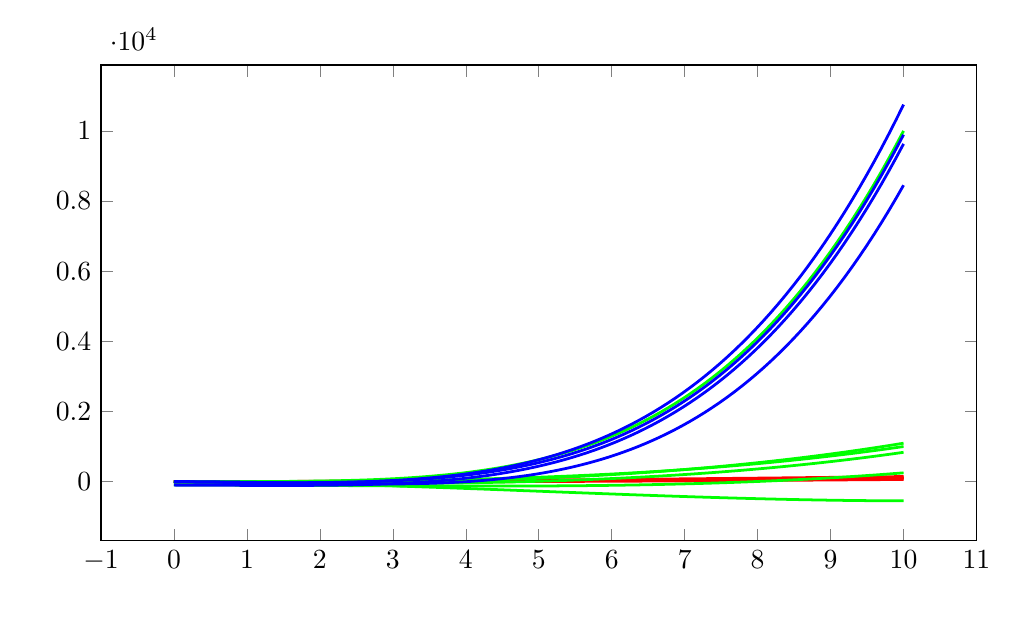
\begin{tikzpicture}[line width=1]
\begin{axis}[width=5in, height=3in,
             scatter/classes={a={mark=*,draw=black}},
             xlabel={\mbox{}},
             xlabel style={name=xlabel}, 
             ylabel={\mbox{}}, 
             legend style={
                at={(xlabel.south)},
                yshift=-1ex,
                anchor=north,
                legend cell align=left,
                },
        ]
]
\addplot[draw=red, line width=1] coordinates {(0.0,0.0)
(0.101,0.0102)
(0.202,0.0408)
(0.303,0.0918)
(0.404,0.1632)
(0.5051,0.2551)
(0.6061,0.3673)
(0.7071,0.4999)
(0.8081,0.653)
(0.9091,0.8264)
(1.0101,1.0203)
(1.1111,1.2346)
(1.2121,1.4692)
(1.3131,1.7243)
(1.4141,1.9998)
(1.5152,2.2957)
(1.6162,2.612)
(1.7172,2.9487)
(1.8182,3.3058)
(1.9192,3.6833)
(2.0202,4.0812)
(2.1212,4.4995)
(2.2222,4.9383)
(2.3232,5.3974)
(2.4242,5.877)
(2.5253,6.3769)
(2.6263,6.8973)
(2.7273,7.438)
(2.8283,7.9992)
(2.9293,8.5808)
(3.0303,9.1827)
(3.1313,9.8051)
(3.2323,10.4479)
(3.3333,11.1111)
(3.4343,11.7947)
(3.5354,12.4987)
(3.6364,13.2231)
(3.7374,13.968)
(3.8384,14.7332)
(3.9394,15.5188)
(4.0404,16.3249)
(4.1414,17.1513)
(4.2424,17.9982)
(4.3434,18.8654)
(4.4444,19.7531)
(4.5455,20.6612)
(4.6465,21.5896)
(4.7475,22.5385)
(4.8485,23.5078)
(4.9495,24.4975)
(5.0505,25.5076)
(5.1515,26.5381)
(5.2525,27.589)
(5.3535,28.6603)
(5.4545,29.7521)
(5.5556,30.8642)
(5.6566,31.9967)
(5.7576,33.1497)
(5.8586,34.323)
(5.9596,35.5168)
(6.0606,36.7309)
(6.1616,37.9655)
(6.2626,39.2205)
(6.3636,40.4959)
(6.4646,41.7917)
(6.5657,43.1078)
(6.6667,44.4444)
(6.7677,45.8014)
(6.8687,47.1789)
(6.9697,48.5767)
(7.0707,49.9949)
(7.1717,51.4335)
(7.2727,52.8926)
(7.3737,54.372)
(7.4747,55.8718)
(7.5758,57.3921)
(7.6768,58.9328)
(7.7778,60.4938)
(7.8788,62.0753)
(7.9798,63.6772)
(8.0808,65.2995)
(8.1818,66.9421)
(8.2828,68.6052)
(8.3838,70.2887)
(8.4848,71.9927)
(8.5859,73.717)
(8.6869,75.4617)
(8.7879,77.2268)
(8.8889,79.0123)
(8.9899,80.8183)
(9.0909,82.6446)
(9.1919,84.4914)
(9.2929,86.3585)
(9.3939,88.2461)
(9.4949,90.1541)
(9.596,92.0824)
(9.697,94.0312)
(9.798,96.0004)
(9.899,97.99)
(10.0,100.0)
(10.0,100.0)};\addplot[draw=red, line width=1] coordinates {(0.0,2.0)
(0.101,2.0102)
(0.202,2.0408)
(0.303,2.0918)
(0.404,2.1632)
(0.5051,2.2551)
(0.6061,2.3673)
(0.7071,2.4999)
(0.8081,2.653)
(0.9091,2.8264)
(1.0101,3.0203)
(1.1111,3.2346)
(1.2121,3.4692)
(1.3131,3.7243)
(1.4141,3.9998)
(1.5152,4.2957)
(1.6162,4.612)
(1.7172,4.9487)
(1.8182,5.3058)
(1.9192,5.6833)
(2.0202,6.0812)
(2.1212,6.4995)
(2.2222,6.9383)
(2.3232,7.3974)
(2.4242,7.877)
(2.5253,8.3769)
(2.6263,8.8973)
(2.7273,9.438)
(2.8283,9.9992)
(2.9293,10.5808)
(3.0303,11.1827)
(3.1313,11.8051)
(3.2323,12.4479)
(3.3333,13.1111)
(3.4343,13.7947)
(3.5354,14.4987)
(3.6364,15.2231)
(3.7374,15.968)
(3.8384,16.7332)
(3.9394,17.5188)
(4.0404,18.3249)
(4.1414,19.1513)
(4.2424,19.9982)
(4.3434,20.8654)
(4.4444,21.7531)
(4.5455,22.6612)
(4.6465,23.5896)
(4.7475,24.5385)
(4.8485,25.5078)
(4.9495,26.4975)
(5.0505,27.5076)
(5.1515,28.5381)
(5.2525,29.589)
(5.3535,30.6603)
(5.4545,31.7521)
(5.5556,32.8642)
(5.6566,33.9967)
(5.7576,35.1497)
(5.8586,36.323)
(5.9596,37.5168)
(6.0606,38.7309)
(6.1616,39.9655)
(6.2626,41.2205)
(6.3636,42.4959)
(6.4646,43.7917)
(6.5657,45.1078)
(6.6667,46.4444)
(6.7677,47.8014)
(6.8687,49.1789)
(6.9697,50.5767)
(7.0707,51.9949)
(7.1717,53.4335)
(7.2727,54.8926)
(7.3737,56.372)
(7.4747,57.8718)
(7.5758,59.3921)
(7.6768,60.9328)
(7.7778,62.4938)
(7.8788,64.0753)
(7.9798,65.6772)
(8.0808,67.2995)
(8.1818,68.9421)
(8.2828,70.6052)
(8.3838,72.2887)
(8.4848,73.9927)
(8.5859,75.717)
(8.6869,77.4617)
(8.7879,79.2268)
(8.8889,81.0123)
(8.9899,82.8183)
(9.0909,84.6446)
(9.1919,86.4914)
(9.2929,88.3585)
(9.3939,90.2461)
(9.4949,92.1541)
(9.596,94.0824)
(9.697,96.0312)
(9.798,98.0004)
(9.899,99.99)
(10.0,102.0)
(10.0,102.0)};\addplot[draw=red, line width=1] coordinates {(0.0,1.0)
(0.101,1.0102)
(0.202,1.0408)
(0.303,1.0918)
(0.404,1.1632)
(0.5051,1.2551)
(0.6061,1.3673)
(0.7071,1.4999)
(0.8081,1.653)
(0.9091,1.8264)
(1.0101,2.0203)
(1.1111,2.2346)
(1.2121,2.4692)
(1.3131,2.7243)
(1.4141,2.9998)
(1.5152,3.2957)
(1.6162,3.612)
(1.7172,3.9487)
(1.8182,4.3058)
(1.9192,4.6833)
(2.0202,5.0812)
(2.1212,5.4995)
(2.2222,5.9383)
(2.3232,6.3974)
(2.4242,6.877)
(2.5253,7.3769)
(2.6263,7.8973)
(2.7273,8.438)
(2.8283,8.9992)
(2.9293,9.5808)
(3.0303,10.1827)
(3.1313,10.8051)
(3.2323,11.4479)
(3.3333,12.1111)
(3.4343,12.7947)
(3.5354,13.4987)
(3.6364,14.2231)
(3.7374,14.968)
(3.8384,15.7332)
(3.9394,16.5188)
(4.0404,17.3249)
(4.1414,18.1513)
(4.2424,18.9982)
(4.3434,19.8654)
(4.4444,20.7531)
(4.5455,21.6612)
(4.6465,22.5896)
(4.7475,23.5385)
(4.8485,24.5078)
(4.9495,25.4975)
(5.0505,26.5076)
(5.1515,27.5381)
(5.2525,28.589)
(5.3535,29.6603)
(5.4545,30.7521)
(5.5556,31.8642)
(5.6566,32.9967)
(5.7576,34.1497)
(5.8586,35.323)
(5.9596,36.5168)
(6.0606,37.7309)
(6.1616,38.9655)
(6.2626,40.2205)
(6.3636,41.4959)
(6.4646,42.7917)
(6.5657,44.1078)
(6.6667,45.4444)
(6.7677,46.8014)
(6.8687,48.1789)
(6.9697,49.5767)
(7.0707,50.9949)
(7.1717,52.4335)
(7.2727,53.8926)
(7.3737,55.372)
(7.4747,56.8718)
(7.5758,58.3921)
(7.6768,59.9328)
(7.7778,61.4938)
(7.8788,63.0753)
(7.9798,64.6772)
(8.0808,66.2995)
(8.1818,67.9421)
(8.2828,69.6052)
(8.3838,71.2887)
(8.4848,72.9927)
(8.5859,74.717)
(8.6869,76.4617)
(8.7879,78.2268)
(8.8889,80.0123)
(8.9899,81.8183)
(9.0909,83.6446)
(9.1919,85.4914)
(9.2929,87.3585)
(9.3939,89.2461)
(9.4949,91.1541)
(9.596,93.0824)
(9.697,95.0312)
(9.798,97.0004)
(9.899,98.99)
(10.0,101.0)
(10.0,101.0)};\addplot[draw=red, line width=1] coordinates {(0.0,-5.0)
(0.101,-4.4847)
(0.202,-3.9491)
(0.303,-3.393)
(0.404,-2.8165)
(0.5051,-2.2197)
(0.6061,-1.6024)
(0.7071,-0.9647)
(0.8081,-0.3066)
(0.9091,0.3719)
(1.0101,1.0708)
(1.1111,1.7901)
(1.2121,2.5298)
(1.3131,3.29)
(1.4141,4.0705)
(1.5152,4.8714)
(1.6162,5.6928)
(1.7172,6.5345)
(1.8182,7.3967)
(1.9192,8.2793)
(2.0202,9.1822)
(2.1212,10.1056)
(2.2222,11.0494)
(2.3232,12.0136)
(2.4242,12.9982)
(2.5253,14.0032)
(2.6263,15.0286)
(2.7273,16.0744)
(2.8283,17.1406)
(2.9293,18.2272)
(3.0303,19.3343)
(3.1313,20.4617)
(3.2323,21.6095)
(3.3333,22.7778)
(3.4343,23.9664)
(3.5354,25.1755)
(3.6364,26.405)
(3.7374,27.6548)
(3.8384,28.9251)
(3.9394,30.2158)
(4.0404,31.5269)
(4.1414,32.8584)
(4.2424,34.2103)
(4.3434,35.5826)
(4.4444,36.9753)
(4.5455,38.3884)
(4.6465,39.822)
(4.7475,41.2759)
(4.8485,42.7502)
(4.9495,44.245)
(5.0505,45.7601)
(5.1515,47.2957)
(5.2525,48.8516)
(5.3535,50.428)
(5.4545,52.0248)
(5.5556,53.642)
(5.6566,55.2796)
(5.7576,56.9376)
(5.8586,58.616)
(5.9596,60.3148)
(6.0606,62.034)
(6.1616,63.7736)
(6.2626,65.5336)
(6.3636,67.314)
(6.4646,69.1149)
(6.5657,70.9361)
(6.6667,72.7778)
(6.7677,74.6398)
(6.8687,76.5223)
(6.9697,78.4252)
(7.0707,80.3484)
(7.1717,82.2921)
(7.2727,84.2562)
(7.3737,86.2407)
(7.4747,88.2456)
(7.5758,90.2709)
(7.6768,92.3166)
(7.7778,94.3827)
(7.8788,96.4692)
(7.9798,98.5762)
(8.0808,100.7035)
(8.1818,102.8512)
(8.2828,105.0194)
(8.3838,107.2079)
(8.4848,109.4169)
(8.5859,111.6463)
(8.6869,113.896)
(8.7879,116.1662)
(8.8889,118.4568)
(8.9899,120.7678)
(9.0909,123.0992)
(9.1919,125.451)
(9.2929,127.8232)
(9.3939,130.2158)
(9.4949,132.6288)
(9.596,135.0622)
(9.697,137.5161)
(9.798,139.9903)
(9.899,142.485)
(10.0,145.0)
(10.0,145.0)};\addplot[draw=red, line width=1] coordinates {(0.0,-8.0)
(0.101,-8.2928)
(0.202,-8.5652)
(0.303,-8.8173)
(0.404,-9.0489)
(0.5051,-9.2601)
(0.6061,-9.4509)
(0.7071,-9.6213)
(0.8081,-9.7712)
(0.9091,-9.9008)
(1.0101,-10.01)
(1.1111,-10.0988)
(1.2121,-10.1671)
(1.3131,-10.2151)
(1.4141,-10.2426)
(1.5152,-10.2498)
(1.6162,-10.2365)
(1.7172,-10.2028)
(1.8182,-10.1488)
(1.9192,-10.0743)
(2.0202,-9.9794)
(2.1212,-9.8641)
(2.2222,-9.7284)
(2.3232,-9.5723)
(2.4242,-9.3958)
(2.5253,-9.1989)
(2.6263,-8.9815)
(2.7273,-8.7438)
(2.8283,-8.4857)
(2.9293,-8.2071)
(3.0303,-7.9082)
(3.1313,-7.5888)
(3.2323,-7.2491)
(3.3333,-6.8889)
(3.4343,-6.5083)
(3.5354,-6.1073)
(3.6364,-5.686)
(3.7374,-5.2442)
(3.8384,-4.782)
(3.9394,-4.2994)
(4.0404,-3.7963)
(4.1414,-3.2729)
(4.2424,-2.7291)
(4.3434,-2.1649)
(4.4444,-1.5802)
(4.5455,-0.9752)
(4.6465,-0.3498)
(4.7475,0.2961)
(4.8485,0.9624)
(4.9495,1.649)
(5.0505,2.3561)
(5.1515,3.0836)
(5.2525,3.8314)
(5.3535,4.5997)
(5.4545,5.3884)
(5.5556,6.1975)
(5.6566,7.027)
(5.7576,7.877)
(5.8586,8.7473)
(5.9596,9.638)
(6.0606,10.5491)
(6.1616,11.4807)
(6.2626,12.4326)
(6.3636,13.405)
(6.4646,14.3977)
(6.5657,15.4109)
(6.6667,16.4444)
(6.7677,17.4984)
(6.8687,18.5728)
(6.9697,19.6676)
(7.0707,20.7828)
(7.1717,21.9184)
(7.2727,23.0744)
(7.3737,24.2508)
(7.4747,25.4476)
(7.5758,26.6648)
(7.6768,27.9025)
(7.7778,29.1605)
(7.8788,30.4389)
(7.9798,31.7378)
(8.0808,33.057)
(8.1818,34.3967)
(8.2828,35.7568)
(8.3838,37.1372)
(8.4848,38.5381)
(8.5859,39.9594)
(8.6869,41.4011)
(8.7879,42.8632)
(8.8889,44.3457)
(8.9899,45.8486)
(9.0909,47.3719)
(9.1919,48.9156)
(9.2929,50.4797)
(9.3939,52.0643)
(9.4949,53.6692)
(9.596,55.2946)
(9.697,56.9403)
(9.798,58.6065)
(9.899,60.293)
(10.0,62.0)
(10.0,62.0)};\addplot[draw=green, line width=1] coordinates {(0.0,0.0)
(0.101,0.001)
(0.202,0.0082)
(0.303,0.0278)
(0.404,0.066)
(0.5051,0.1288)
(0.6061,0.2226)
(0.7071,0.3535)
(0.8081,0.5277)
(0.9091,0.7513)
(1.0101,1.0306)
(1.1111,1.3717)
(1.2121,1.7809)
(1.3131,2.2643)
(1.4141,2.828)
(1.5152,3.4783)
(1.6162,4.2214)
(1.7172,5.0634)
(1.8182,6.0105)
(1.9192,7.069)
(2.0202,8.2449)
(2.1212,9.5445)
(2.2222,10.9739)
(2.3232,12.5394)
(2.4242,14.2472)
(2.5253,16.1033)
(2.6263,18.114)
(2.7273,20.2855)
(2.8283,22.624)
(2.9293,25.1356)
(3.0303,27.8265)
(3.1313,30.7029)
(3.2323,33.771)
(3.3333,37.037)
(3.4343,40.5071)
(3.5354,44.1874)
(3.6364,48.0841)
(3.7374,52.2035)
(3.8384,56.5516)
(3.9394,61.1348)
(4.0404,65.959)
(4.1414,71.0307)
(4.2424,76.3558)
(4.3434,81.9407)
(4.4444,87.7915)
(4.5455,93.9144)
(4.6465,100.3155)
(4.7475,107.001)
(4.8485,113.9772)
(4.9495,121.2503)
(5.0505,128.8263)
(5.1515,136.7115)
(5.2525,144.912)
(5.3535,153.4341)
(5.4545,162.284)
(5.5556,171.4678)
(5.6566,180.9916)
(5.7576,190.8618)
(5.8586,201.0844)
(5.9596,211.6657)
(6.0606,222.6118)
(6.1616,233.9289)
(6.2626,245.6233)
(6.3636,257.701)
(6.4646,270.1683)
(6.5657,283.0313)
(6.6667,296.2963)
(6.7677,309.9694)
(6.8687,324.0568)
(6.9697,338.5647)
(7.0707,353.4993)
(7.1717,368.8667)
(7.2727,384.6732)
(7.3737,400.9249)
(7.4747,417.628)
(7.5758,434.7887)
(7.6768,452.4131)
(7.7778,470.5075)
(7.8788,489.0781)
(7.9798,508.131)
(8.0808,527.6724)
(8.1818,547.7085)
(8.2828,568.2455)
(8.3838,589.2895)
(8.4848,610.8468)
(8.5859,632.9235)
(8.6869,655.5258)
(8.7879,678.6599)
(8.8889,702.332)
(8.9899,726.5482)
(9.0909,751.3148)
(9.1919,776.6379)
(9.2929,802.5238)
(9.3939,828.9785)
(9.4949,856.0083)
(9.596,883.6194)
(9.697,911.8179)
(9.798,940.6101)
(9.899,970.002)
(10.0,1000.0)
(10.0,1000.0)};\addplot[draw=green, line width=1] coordinates {(0.0,-5.0)
(0.101,-6.9886)
(0.202,-8.9097)
(0.303,-10.7573)
(0.404,-12.5251)
(0.5051,-14.207)
(0.6061,-15.7967)
(0.7071,-17.2881)
(0.8081,-18.675)
(0.9091,-19.9512)
(1.0101,-21.1105)
(1.1111,-22.1468)
(1.2121,-23.0538)
(1.3131,-23.8254)
(1.4141,-24.4554)
(1.5152,-24.9377)
(1.6162,-25.2659)
(1.7172,-25.434)
(1.8182,-25.4358)
(1.9192,-25.265)
(2.0202,-24.9155)
(2.1212,-24.3811)
(2.2222,-23.6557)
(2.3232,-22.733)
(2.4242,-21.6068)
(2.5253,-20.2711)
(2.6263,-18.7195)
(2.7273,-16.9459)
(2.8283,-14.9442)
(2.9293,-12.708)
(3.0303,-10.2314)
(3.1313,-7.508)
(3.2323,-4.5317)
(3.3333,-1.2963)
(3.4343,2.2044)
(3.5354,5.9765)
(3.6364,10.0263)
(3.7374,14.3599)
(3.8384,18.9835)
(3.9394,23.9034)
(4.0404,29.1256)
(4.1414,34.6563)
(4.2424,40.5019)
(4.3434,46.6683)
(4.4444,53.1619)
(4.5455,59.9887)
(4.6465,67.1551)
(4.7475,74.6671)
(4.8485,82.531)
(4.9495,90.7529)
(5.0505,99.339)
(5.1515,108.2955)
(5.2525,117.6286)
(5.3535,127.3445)
(5.4545,137.4493)
(5.5556,147.9492)
(5.6566,158.8505)
(5.7576,170.1593)
(5.8586,181.8818)
(5.9596,194.0241)
(6.0606,206.5925)
(6.1616,219.5931)
(6.2626,233.0322)
(6.3636,246.9159)
(6.4646,261.2503)
(6.5657,276.0417)
(6.6667,291.2963)
(6.7677,307.0202)
(6.8687,323.2197)
(6.9697,339.9008)
(7.0707,357.0698)
(7.1717,374.7329)
(7.2727,392.8963)
(7.3737,411.5661)
(7.4747,430.7486)
(7.5758,450.4498)
(7.6768,470.6761)
(7.7778,491.4335)
(7.8788,512.7282)
(7.9798,534.5666)
(8.0808,556.9546)
(8.1818,579.8986)
(8.2828,603.4046)
(8.3838,627.479)
(8.4848,652.1278)
(8.5859,677.3572)
(8.6869,703.1735)
(8.7879,729.5827)
(8.8889,756.5912)
(8.9899,784.2051)
(9.0909,812.4305)
(9.1919,841.2737)
(9.2929,870.7408)
(9.3939,900.838)
(9.4949,931.5715)
(9.596,962.9475)
(9.697,994.9722)
(9.798,1027.6517)
(9.899,1060.9922)
(10.0,1095.0)
(10.0,1095.0)};\addplot[draw=green, line width=1] coordinates {(0.0,-15.0)
(0.101,-17.514)
(0.202,-20.0014)
(0.303,-22.4561)
(0.404,-24.8718)
(0.5051,-27.2424)
(0.6061,-29.5616)
(0.7071,-31.8233)
(0.8081,-34.0214)
(0.9091,-36.1495)
(1.0101,-38.2016)
(1.1111,-40.1715)
(1.2121,-42.0529)
(1.3131,-43.8397)
(1.4141,-45.5257)
(1.5152,-47.1048)
(1.6162,-48.5707)
(1.7172,-49.9172)
(1.8182,-51.1382)
(1.9192,-52.2275)
(2.0202,-53.179)
(2.1212,-53.9863)
(2.2222,-54.6433)
(2.3232,-55.144)
(2.4242,-55.482)
(2.5253,-55.6511)
(2.6263,-55.6453)
(2.7273,-55.4583)
(2.8283,-55.0839)
(2.9293,-54.516)
(3.0303,-53.7484)
(3.1313,-52.7748)
(3.2323,-51.5891)
(3.3333,-50.1852)
(3.4343,-48.5568)
(3.5354,-46.6977)
(3.6364,-44.6018)
(3.7374,-42.2629)
(3.8384,-39.6748)
(3.9394,-36.8313)
(4.0404,-33.7262)
(4.1414,-30.3534)
(4.2424,-26.7066)
(4.3434,-22.7797)
(4.4444,-18.5665)
(4.5455,-14.0609)
(4.6465,-9.2565)
(4.7475,-4.1473)
(4.8485,1.2729)
(4.9495,7.0104)
(5.0505,13.0712)
(5.1515,19.4617)
(5.2525,26.1879)
(5.3535,33.2561)
(5.4545,40.6724)
(5.5556,48.4431)
(5.6566,56.5742)
(5.7576,65.0721)
(5.8586,73.9428)
(5.9596,83.1926)
(6.0606,92.8276)
(6.1616,102.854)
(6.2626,113.2781)
(6.3636,124.1059)
(6.4646,135.3438)
(6.5657,146.9977)
(6.6667,159.0741)
(6.7677,171.5789)
(6.8687,184.5185)
(6.9697,197.899)
(7.0707,211.7265)
(7.1717,226.0073)
(7.2727,240.7476)
(7.3737,255.9534)
(7.4747,271.6311)
(7.5758,287.7868)
(7.6768,304.4267)
(7.7778,321.5569)
(7.8788,339.1837)
(7.9798,357.3132)
(8.0808,375.9517)
(8.1818,395.1052)
(8.2828,414.78)
(8.3838,434.9823)
(8.4848,455.7182)
(8.5859,476.994)
(8.6869,498.8157)
(8.7879,521.1897)
(8.8889,544.1221)
(8.9899,567.619)
(9.0909,591.6867)
(9.1919,616.3313)
(9.2929,641.5591)
(9.3939,667.3761)
(9.4949,693.7886)
(9.596,720.8028)
(9.697,748.4249)
(9.798,776.661)
(9.899,805.5173)
(10.0,835.0)
(10.0,835.0)};\addplot[draw=green, line width=1] coordinates {(0.0,1.0)
(0.101,0.3429)
(0.202,-0.614)
(0.303,-1.8647)
(0.404,-3.403)
(0.5051,-5.2226)
(0.6061,-7.3173)
(0.7071,-9.6811)
(0.8081,-12.3077)
(0.9091,-15.1908)
(1.0101,-18.3245)
(1.1111,-21.7023)
(1.2121,-25.3183)
(1.3131,-29.1661)
(1.4141,-33.2397)
(1.5152,-37.5327)
(1.6162,-42.0391)
(1.7172,-46.7527)
(1.8182,-51.6672)
(1.9192,-56.7765)
(2.0202,-62.0744)
(2.1212,-67.5547)
(2.2222,-73.2112)
(2.3232,-79.0379)
(2.4242,-85.0283)
(2.5253,-91.1765)
(2.6263,-97.4761)
(2.7273,-103.9211)
(2.8283,-110.5052)
(2.9293,-117.2223)
(3.0303,-124.0661)
(3.1313,-131.0305)
(3.2323,-138.1093)
(3.3333,-145.2963)
(3.4343,-152.5853)
(3.5354,-159.9702)
(3.6364,-167.4448)
(3.7374,-175.0028)
(3.8384,-182.6381)
(3.9394,-190.3446)
(4.0404,-198.1159)
(4.1414,-205.9461)
(4.2424,-213.8287)
(4.3434,-221.7578)
(4.4444,-229.727)
(4.5455,-237.7303)
(4.6465,-245.7614)
(4.7475,-253.8141)
(4.8485,-261.8823)
(4.9495,-269.9597)
(5.0505,-278.0403)
(5.1515,-286.1177)
(5.2525,-294.1859)
(5.3535,-302.2386)
(5.4545,-310.2697)
(5.5556,-318.273)
(5.6566,-326.2422)
(5.7576,-334.1713)
(5.8586,-342.0539)
(5.9596,-349.8841)
(6.0606,-357.6554)
(6.1616,-365.3619)
(6.2626,-372.9972)
(6.3636,-380.5552)
(6.4646,-388.0298)
(6.5657,-395.4147)
(6.6667,-402.7037)
(6.7677,-409.8907)
(6.8687,-416.9695)
(6.9697,-423.9339)
(7.0707,-430.7777)
(7.1717,-437.4948)
(7.2727,-444.0789)
(7.3737,-450.5239)
(7.4747,-456.8235)
(7.5758,-462.9717)
(7.6768,-468.9621)
(7.7778,-474.7888)
(7.8788,-480.4453)
(7.9798,-485.9256)
(8.0808,-491.2235)
(8.1818,-496.3328)
(8.2828,-501.2473)
(8.3838,-505.9609)
(8.4848,-510.4673)
(8.5859,-514.7603)
(8.6869,-518.8339)
(8.7879,-522.6817)
(8.8889,-526.2977)
(8.9899,-529.6755)
(9.0909,-532.8092)
(9.1919,-535.6923)
(9.2929,-538.3189)
(9.3939,-540.6827)
(9.4949,-542.7774)
(9.596,-544.597)
(9.697,-546.1353)
(9.798,-547.386)
(9.899,-548.3429)
(10.0,-549.0)
(10.0,-549.0)};\addplot[draw=green, line width=1] coordinates {(0.0,-100.0)
(0.101,-99.5653)
(0.202,-99.2673)
(0.303,-99.0998)
(0.404,-99.0566)
(0.5051,-99.1315)
(0.6061,-99.3183)
(0.7071,-99.6108)
(0.8081,-100.0029)
(0.9091,-100.4884)
(1.0101,-101.061)
(1.1111,-101.7147)
(1.2121,-102.4432)
(1.3131,-103.2403)
(1.4141,-104.0999)
(1.5152,-105.0157)
(1.6162,-105.9817)
(1.7172,-106.9915)
(1.8182,-108.0391)
(1.9192,-109.1182)
(2.0202,-110.2226)
(2.1212,-111.3462)
(2.2222,-112.4829)
(2.3232,-113.6263)
(2.4242,-114.7703)
(2.5253,-115.9088)
(2.6263,-117.0355)
(2.7273,-118.1443)
(2.8283,-119.2289)
(2.9293,-120.2833)
(3.0303,-121.3012)
(3.1313,-122.2764)
(3.2323,-123.2027)
(3.3333,-124.0741)
(3.4343,-124.8842)
(3.5354,-125.6269)
(3.6364,-126.296)
(3.7374,-126.8854)
(3.8384,-127.3888)
(3.9394,-127.8)
(4.0404,-128.113)
(4.1414,-128.3214)
(4.2424,-128.4192)
(4.3434,-128.4001)
(4.4444,-128.2579)
(4.5455,-127.9865)
(4.6465,-127.5796)
(4.7475,-127.0312)
(4.8485,-126.335)
(4.9495,-125.4848)
(5.0505,-124.4744)
(5.1515,-123.2977)
(5.2525,-121.9485)
(5.3535,-120.4206)
(5.4545,-118.7077)
(5.5556,-116.8038)
(5.6566,-114.7027)
(5.7576,-112.3981)
(5.8586,-109.8839)
(5.9596,-107.1538)
(6.0606,-104.2018)
(6.1616,-101.0216)
(6.2626,-97.607)
(6.3636,-93.9519)
(6.4646,-90.0501)
(6.5657,-85.8953)
(6.6667,-81.4815)
(6.7677,-76.8024)
(6.8687,-71.8518)
(6.9697,-66.6235)
(7.0707,-61.1115)
(7.1717,-55.3094)
(7.2727,-49.2111)
(7.3737,-42.8105)
(7.4747,-36.1012)
(7.5758,-29.0773)
(7.6768,-21.7324)
(7.7778,-14.0604)
(7.8788,-6.055)
(7.9798,2.2898)
(8.0808,10.9802)
(8.1818,20.0225)
(8.2828,29.4229)
(8.3838,39.1875)
(8.4848,49.3224)
(8.5859,59.834)
(8.6869,70.7283)
(8.7879,82.0116)
(8.8889,93.69)
(8.9899,105.7697)
(9.0909,118.2569)
(9.1919,131.1579)
(9.2929,144.4787)
(9.3939,158.2255)
(9.4949,172.4046)
(9.596,187.0221)
(9.697,202.0842)
(9.798,217.5971)
(9.899,233.567)
(10.0,250.0)
(10.0,250.0)};\addplot[draw=green, line width=1] coordinates {(0.0,0.0)
(0.101,0.0001)
(0.202,0.0017)
(0.303,0.0084)
(0.404,0.0267)
(0.5051,0.0651)
(0.6061,0.1349)
(0.7071,0.2499)
(0.8081,0.4264)
(0.9091,0.683)
(1.0101,1.041)
(1.1111,1.5242)
(1.2121,2.1587)
(1.3131,2.9733)
(1.4141,3.9992)
(1.5152,5.2702)
(1.6162,6.8224)
(1.7172,8.6947)
(1.8182,10.9282)
(1.9192,13.5667)
(2.0202,16.6563)
(2.1212,20.2459)
(2.2222,24.3865)
(2.3232,29.132)
(2.4242,34.5386)
(2.5253,40.6649)
(2.6263,47.5721)
(2.7273,55.3241)
(2.8283,63.9869)
(2.9293,73.6294)
(3.0303,84.3226)
(3.1313,96.1404)
(3.2323,109.1589)
(3.3333,123.4568)
(3.4343,139.1153)
(3.5354,156.2181)
(3.6364,174.8514)
(3.7374,195.104)
(3.8384,217.0669)
(3.9394,240.8339)
(4.0404,266.5012)
(4.1414,294.1675)
(4.2424,323.9339)
(4.3434,355.9041)
(4.4444,390.1844)
(4.5455,426.8834)
(4.6465,466.1123)
(4.7475,507.9847)
(4.8485,552.6169)
(4.9495,600.1275)
(5.0505,650.6377)
(5.1515,704.2712)
(5.2525,761.1541)
(5.3535,821.4151)
(5.4545,885.1854)
(5.5556,952.5987)
(5.6566,1023.7911)
(5.7576,1098.9012)
(5.8586,1178.0703)
(5.9596,1261.4419)
(6.0606,1349.1624)
(6.1616,1441.3802)
(6.2626,1538.2467)
(6.3636,1639.9153)
(6.4646,1746.5423)
(6.5657,1858.2864)
(6.6667,1975.3086)
(6.7677,2097.7727)
(6.8687,2225.8448)
(6.9697,2359.6934)
(7.0707,2499.4899)
(7.1717,2645.4077)
(7.2727,2797.6231)
(7.3737,2956.3147)
(7.4747,3121.6636)
(7.5758,3293.8535)
(7.6768,3473.0704)
(7.7778,3659.5031)
(7.8788,3853.3427)
(7.9798,4054.7827)
(8.0808,4264.0194)
(8.1818,4481.2513)
(8.2828,4706.6796)
(8.3838,4940.5078)
(8.4848,5182.9422)
(8.5859,5434.1913)
(8.6869,5694.4663)
(8.7879,5963.9807)
(8.8889,6242.9508)
(8.9899,6531.595)
(9.0909,6830.1346)
(9.1919,7138.793)
(9.2929,7457.7965)
(9.3939,7787.3737)
(9.4949,8127.7556)
(9.596,8479.1759)
(9.697,8841.8706)
(9.798,9216.0784)
(9.899,9602.0403)
(10.0,10000.0)
(10.0,10000.0)};\addplot[draw=blue, line width=1] coordinates {(0.0,-9.0)
(0.101,-11.0099)
(0.202,-12.9979)
(0.303,-14.9603)
(0.404,-16.8909)
(0.5051,-18.7809)
(0.6061,-20.619)
(0.7071,-22.3915)
(0.8081,-24.0822)
(0.9091,-25.6724)
(1.0101,-27.1407)
(1.1111,-28.4635)
(1.2121,-29.6145)
(1.3131,-30.5651)
(1.4141,-31.2838)
(1.5152,-31.7372)
(1.6162,-31.8888)
(1.7172,-31.7)
(1.8182,-31.1296)
(1.9192,-30.1339)
(2.0202,-28.6665)
(2.1212,-26.6788)
(2.2222,-24.1196)
(2.3232,-20.9352)
(2.4242,-17.0693)
(2.5253,-12.4633)
(2.6263,-7.0559)
(2.7273,-0.7833)
(2.8283,6.4205)
(2.9293,14.6243)
(3.0303,23.8993)
(3.1313,34.3193)
(3.2323,45.9603)
(3.3333,58.9012)
(3.4343,73.2231)
(3.5354,89.0098)
(3.6364,106.3473)
(3.7374,125.3245)
(3.8384,146.0324)
(3.9394,168.5649)
(4.0404,193.018)
(4.1414,219.4905)
(4.2424,248.0836)
(4.3434,278.9009)
(4.4444,312.0486)
(4.5455,347.6355)
(4.6465,385.7726)
(4.7475,426.5737)
(4.8485,470.155)
(4.9495,516.6351)
(5.0505,566.1352)
(5.1515,618.779)
(5.2525,674.6926)
(5.3535,734.0048)
(5.4545,796.8466)
(5.5556,863.3518)
(5.6566,933.6565)
(5.7576,1007.8994)
(5.8586,1086.2216)
(5.9596,1168.7668)
(6.0606,1255.6812)
(6.1616,1347.1134)
(6.2626,1443.2146)
(6.3636,1544.1384)
(6.4646,1650.0411)
(6.5657,1761.0811)
(6.6667,1877.4198)
(6.7677,1999.2206)
(6.8687,2126.6499)
(6.9697,2259.8762)
(7.0707,2399.0706)
(7.1717,2544.4069)
(7.2727,2696.0611)
(7.3737,2854.212)
(7.4747,3019.0405)
(7.5758,3190.7304)
(7.6768,3369.4678)
(7.7778,3555.4414)
(7.8788,3748.8422)
(7.9798,3949.8639)
(8.0808,4158.7027)
(8.1818,4375.5571)
(8.2828,4600.6282)
(8.3838,4834.1198)
(8.4848,5076.2379)
(8.5859,5327.1911)
(8.6869,5587.1906)
(8.7879,5856.45)
(8.8889,6135.1853)
(8.9899,6423.6153)
(9.0909,6721.961)
(9.1919,7030.446)
(9.2929,7349.2965)
(9.3939,7678.741)
(9.4949,8019.0107)
(9.596,8370.3391)
(9.697,8732.9624)
(9.798,9107.1192)
(9.899,9493.0505)
(10.0,9891.0)
(10.0,9891.0)};\addplot[draw=blue, line width=1] coordinates {(0.0,-1.0)
(0.101,-3.5241)
(0.202,-6.0406)
(0.303,-8.5395)
(0.404,-11.0084)
(0.5051,-13.4324)
(0.6061,-15.794)
(0.7071,-18.0733)
(0.8081,-20.2479)
(0.9091,-22.2929)
(1.0101,-24.1809)
(1.1111,-25.8819)
(1.2121,-27.3635)
(1.3131,-28.5908)
(1.4141,-29.5264)
(1.5152,-30.1303)
(1.6162,-30.3602)
(1.7172,-30.1712)
(1.8182,-29.5158)
(1.9192,-28.3442)
(2.0202,-26.6038)
(2.1212,-24.24)
(2.2222,-21.1951)
(2.3232,-17.4094)
(2.4242,-12.8203)
(2.5253,-7.3632)
(2.6263,-0.9704)
(2.7273,6.4278)
(2.8283,14.9038)
(2.9293,24.5326)
(3.0303,35.3915)
(3.1313,47.5605)
(3.2323,61.1218)
(3.3333,76.1605)
(3.4343,92.7638)
(3.5354,111.0217)
(3.6364,131.0265)
(3.7374,152.8731)
(3.8384,176.6589)
(3.9394,202.4838)
(4.0404,230.4502)
(4.1414,260.6628)
(4.2424,293.2291)
(4.3434,328.259)
(4.4444,365.8648)
(4.5455,406.1614)
(4.6465,449.2661)
(4.7475,495.2989)
(4.8485,544.382)
(4.9495,596.6404)
(5.0505,652.2014)
(5.1515,711.1948)
(5.2525,773.753)
(5.3535,840.0109)
(5.4545,910.1058)
(5.5556,984.1776)
(5.6566,1062.3685)
(5.7576,1144.8236)
(5.8586,1231.69)
(5.9596,1323.1177)
(6.0606,1419.259)
(6.1616,1520.2688)
(6.2626,1626.3043)
(6.3636,1737.5254)
(6.4646,1854.0944)
(6.5657,1976.1763)
(6.6667,2103.9383)
(6.7677,2237.5502)
(6.8687,2377.1844)
(6.9697,2523.0157)
(7.0707,2675.2215)
(7.1717,2833.9815)
(7.2727,2999.4781)
(7.3737,3171.8961)
(7.4747,3351.4229)
(7.5758,3538.2482)
(7.6768,3732.5644)
(7.7778,3934.5662)
(7.8788,4144.4511)
(7.9798,4362.4188)
(8.0808,4588.6716)
(8.1818,4823.4143)
(8.2828,5066.8543)
(8.3838,5319.2013)
(8.4848,5580.6678)
(8.5859,5851.4683)
(8.6869,6131.8203)
(8.7879,6421.9436)
(8.8889,6722.0605)
(8.9899,7032.3957)
(9.0909,7353.1766)
(9.1919,7684.633)
(9.2929,8026.9971)
(9.3939,8380.5037)
(9.4949,8745.3902)
(9.596,9121.8963)
(9.697,9510.2642)
(9.798,9910.7389)
(9.899,10323.5676)
(10.0,10749.0)
(10.0,10749.0)};\addplot[draw=blue, line width=1] coordinates {(0.0,1.0)
(0.101,0.342)
(0.202,-0.6206)
(0.303,-1.8841)
(0.404,-3.4423)
(0.5051,-5.2863)
(0.6061,-7.405)
(0.7071,-9.7846)
(0.8081,-12.4089)
(0.9091,-15.2591)
(1.0101,-18.314)
(1.1111,-21.5499)
(1.2121,-24.9405)
(1.3131,-28.4571)
(1.4141,-32.0685)
(1.5152,-35.7409)
(1.6162,-39.4381)
(1.7172,-43.1213)
(1.8182,-46.7495)
(1.9192,-50.2787)
(2.0202,-53.6629)
(2.1212,-56.8533)
(2.2222,-59.7987)
(2.3232,-62.4453)
(2.4242,-64.7369)
(2.5253,-66.6149)
(2.6263,-68.018)
(2.7273,-68.8825)
(2.8283,-69.1422)
(2.9293,-68.7284)
(3.0303,-67.5699)
(3.1313,-65.593)
(3.2323,-62.7214)
(3.3333,-58.8765)
(3.4343,-53.9771)
(3.5354,-47.9395)
(3.6364,-40.6775)
(3.7374,-32.1023)
(3.8384,-22.1229)
(3.9394,-10.6454)
(4.0404,2.4262)
(4.1414,17.1907)
(4.2424,33.7493)
(4.3434,52.2056)
(4.4444,72.6659)
(4.5455,95.2388)
(4.6465,120.0355)
(4.7475,147.1696)
(4.8485,176.7574)
(4.9495,208.9175)
(5.0505,243.7712)
(5.1515,281.442)
(5.2525,322.0562)
(5.3535,365.7423)
(5.4545,412.6317)
(5.5556,462.8579)
(5.6566,516.5572)
(5.7576,573.8681)
(5.8586,634.9319)
(5.9596,699.8922)
(6.0606,768.8952)
(6.1616,842.0894)
(6.2626,919.6262)
(6.3636,1001.6591)
(6.4646,1088.3443)
(6.5657,1179.8404)
(6.6667,1276.3086)
(6.7677,1377.9126)
(6.8687,1484.8184)
(6.9697,1597.1948)
(7.0707,1715.2129)
(7.1717,1839.0462)
(7.2727,1968.871)
(7.3737,2104.866)
(7.4747,2247.2121)
(7.5758,2396.0931)
(7.6768,2551.6952)
(7.7778,2714.2068)
(7.8788,2883.8193)
(7.9798,3060.7261)
(8.0808,3245.1234)
(8.1818,3437.21)
(8.2828,3637.1867)
(8.3838,3845.2574)
(8.4848,4061.6282)
(8.5859,4286.5075)
(8.6869,4520.1066)
(8.7879,4762.6391)
(8.8889,5014.3211)
(8.9899,5275.3713)
(9.0909,5546.0106)
(9.1919,5826.4628)
(9.2929,6116.9539)
(9.3939,6417.7125)
(9.4949,6728.9699)
(9.596,7050.9595)
(9.697,7383.9174)
(9.798,7728.0823)
(9.899,8083.6953)
(10.0,8451.0)
(10.0,8451.0)};\addplot[draw=blue, line width=1] coordinates {(0.0,-100.0)
(0.101,-100.7274)
(0.202,-101.4941)
(0.303,-102.2964)
(0.404,-103.1281)
(0.5051,-103.9804)
(0.6061,-104.8421)
(0.7071,-105.6994)
(0.8081,-106.5362)
(0.9091,-107.3335)
(1.0101,-108.0703)
(1.1111,-108.7228)
(1.2121,-109.2647)
(1.3131,-109.6673)
(1.4141,-109.8994)
(1.5152,-109.9273)
(1.6162,-109.7147)
(1.7172,-109.2229)
(1.8182,-108.4106)
(1.9192,-107.2343)
(2.0202,-105.6475)
(2.1212,-103.6017)
(2.2222,-101.0456)
(2.3232,-97.9254)
(2.4242,-94.185)
(2.5253,-89.7657)
(2.6263,-84.6062)
(2.7273,-78.6429)
(2.8283,-71.8094)
(2.9293,-64.0372)
(3.0303,-55.2549)
(3.1313,-45.389)
(3.2323,-34.3632)
(3.3333,-22.0988)
(3.4343,-8.5145)
(3.5354,6.4732)
(3.6364,22.9506)
(3.7374,41.0064)
(3.8384,60.7318)
(3.9394,82.2205)
(4.0404,105.5687)
(4.1414,130.875)
(4.2424,158.2406)
(4.3434,187.7693)
(4.4444,219.5671)
(4.5455,253.7429)
(4.6465,290.4078)
(4.7475,329.6754)
(4.8485,371.6619)
(4.9495,416.4861)
(5.0505,464.269)
(5.1515,515.1344)
(5.2525,569.2084)
(5.3535,626.6197)
(5.4545,687.4995)
(5.5556,751.9814)
(5.6566,820.2016)
(5.7576,892.2988)
(5.8586,968.4141)
(5.9596,1048.6912)
(6.0606,1133.2762)
(6.1616,1222.3179)
(6.2626,1315.9673)
(6.3636,1414.3781)
(6.4646,1517.7065)
(6.5657,1626.1111)
(6.6667,1739.7531)
(6.7677,1858.7961)
(6.8687,1983.4062)
(6.9697,2113.7522)
(7.0707,2250.0051)
(7.1717,2392.3386)
(7.2727,2540.9289)
(7.3737,2695.9545)
(7.4747,2857.5967)
(7.5758,3026.039)
(7.6768,3201.4675)
(7.7778,3384.071)
(7.8788,3574.0406)
(7.9798,3771.5698)
(8.0808,3976.8548)
(8.1818,4190.0943)
(8.2828,4411.4893)
(8.3838,4641.2435)
(8.4848,4879.563)
(8.5859,5126.6564)
(8.6869,5382.7348)
(8.7879,5648.012)
(8.8889,5922.7039)
(8.9899,6207.0291)
(9.0909,6501.2089)
(9.1919,6805.4668)
(9.2929,7120.029)
(9.3939,7445.1239)
(9.4949,7780.9828)
(9.596,8127.8393)
(9.697,8485.9293)
(9.798,8855.4917)
(9.899,9236.7674)
(10.0,9630.0)
(10.0,9630.0)};
\end{axis}\end{tikzpicture}\end{center}


Notice that the growth behavior of these functions are now clearer.
Now if I increase the domain to $0 \leq n \leq 100$, we see:
%-*-latex-*-

\begin{center}
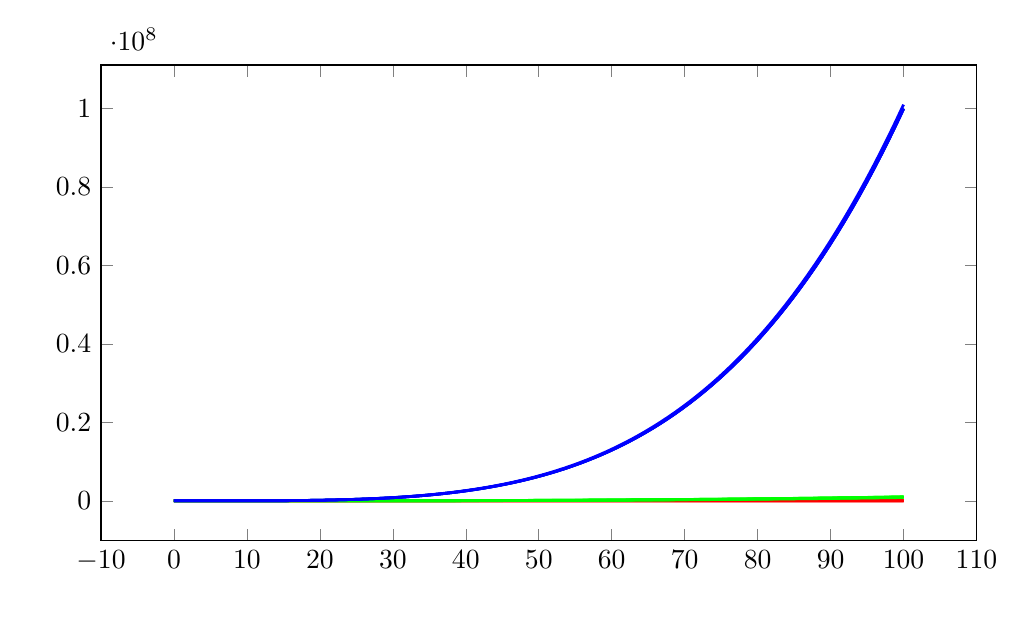
\begin{tikzpicture}[line width=1]
\begin{axis}[width=5in, height=3in,
             scatter/classes={a={mark=*,draw=black}},
             xlabel={\mbox{}},
             xlabel style={name=xlabel}, 
             ylabel={\mbox{}}, 
             legend style={
                at={(xlabel.south)},
                yshift=-1ex,
                anchor=north,
                legend cell align=left,
                },
        ]
]
\addplot[draw=red, line width=1] coordinates {(0.0,0.0)
(1.0101,1.0203)
(2.0202,4.0812)
(3.0303,9.1827)
(4.0404,16.3249)
(5.0505,25.5076)
(6.0606,36.7309)
(7.0707,49.9949)
(8.0808,65.2995)
(9.0909,82.6446)
(10.101,102.0304)
(11.1111,123.4568)
(12.1212,146.9238)
(13.1313,172.4314)
(14.1414,199.9796)
(15.1515,229.5684)
(16.1616,261.1978)
(17.1717,294.8679)
(18.1818,330.5785)
(19.1919,368.3298)
(20.202,408.1216)
(21.2121,449.9541)
(22.2222,493.8272)
(23.2323,539.7408)
(24.2424,587.6951)
(25.2525,637.69)
(26.2626,689.7255)
(27.2727,743.8017)
(28.2828,799.9184)
(29.2929,858.0757)
(30.303,918.2736)
(31.3131,980.5122)
(32.3232,1044.7913)
(33.3333,1111.1111)
(34.3434,1179.4715)
(35.3535,1249.8725)
(36.3636,1322.314)
(37.3737,1396.7962)
(38.3838,1473.319)
(39.3939,1551.8825)
(40.404,1632.4865)
(41.4141,1715.1311)
(42.4242,1799.8163)
(43.4343,1886.5422)
(44.4444,1975.3086)
(45.4545,2066.1157)
(46.4646,2158.9634)
(47.4747,2253.8516)
(48.4848,2350.7805)
(49.4949,2449.75)
(50.5051,2550.7601)
(51.5152,2653.8108)
(52.5253,2758.9022)
(53.5354,2866.0341)
(54.5455,2975.2066)
(55.5556,3086.4198)
(56.5657,3199.6735)
(57.5758,3314.9679)
(58.5859,3432.3028)
(59.596,3551.6784)
(60.6061,3673.0946)
(61.6162,3796.5514)
(62.6263,3922.0488)
(63.6364,4049.5868)
(64.6465,4179.1654)
(65.6566,4310.7846)
(66.6667,4444.4444)
(67.6768,4580.1449)
(68.6869,4717.8859)
(69.697,4857.6676)
(70.7071,4999.4898)
(71.7172,5143.3527)
(72.7273,5289.2562)
(73.7374,5437.2003)
(74.7475,5587.185)
(75.7576,5739.2103)
(76.7677,5893.2762)
(77.7778,6049.3827)
(78.7879,6207.5298)
(79.798,6367.7176)
(80.8081,6529.9459)
(81.8182,6694.2149)
(82.8283,6860.5244)
(83.8384,7028.8746)
(84.8485,7199.2654)
(85.8586,7371.6968)
(86.8687,7546.1688)
(87.8788,7722.6814)
(88.8889,7901.2346)
(89.899,8081.8284)
(90.9091,8264.4628)
(91.9192,8449.1378)
(92.9293,8635.8535)
(93.9394,8824.6097)
(94.9495,9015.4066)
(95.9596,9208.2441)
(96.9697,9403.1221)
(97.9798,9600.0408)
(98.9899,9799.0001)
(100.0,10000.0)};\addplot[draw=red, line width=1] coordinates {(0.0,2.0)
(1.0101,3.0203)
(2.0202,6.0812)
(3.0303,11.1827)
(4.0404,18.3249)
(5.0505,27.5076)
(6.0606,38.7309)
(7.0707,51.9949)
(8.0808,67.2995)
(9.0909,84.6446)
(10.101,104.0304)
(11.1111,125.4568)
(12.1212,148.9238)
(13.1313,174.4314)
(14.1414,201.9796)
(15.1515,231.5684)
(16.1616,263.1978)
(17.1717,296.8679)
(18.1818,332.5785)
(19.1919,370.3298)
(20.202,410.1216)
(21.2121,451.9541)
(22.2222,495.8272)
(23.2323,541.7408)
(24.2424,589.6951)
(25.2525,639.69)
(26.2626,691.7255)
(27.2727,745.8017)
(28.2828,801.9184)
(29.2929,860.0757)
(30.303,920.2736)
(31.3131,982.5122)
(32.3232,1046.7913)
(33.3333,1113.1111)
(34.3434,1181.4715)
(35.3535,1251.8725)
(36.3636,1324.314)
(37.3737,1398.7962)
(38.3838,1475.319)
(39.3939,1553.8825)
(40.404,1634.4865)
(41.4141,1717.1311)
(42.4242,1801.8163)
(43.4343,1888.5422)
(44.4444,1977.3086)
(45.4545,2068.1157)
(46.4646,2160.9634)
(47.4747,2255.8516)
(48.4848,2352.7805)
(49.4949,2451.75)
(50.5051,2552.7601)
(51.5152,2655.8108)
(52.5253,2760.9022)
(53.5354,2868.0341)
(54.5455,2977.2066)
(55.5556,3088.4198)
(56.5657,3201.6735)
(57.5758,3316.9679)
(58.5859,3434.3028)
(59.596,3553.6784)
(60.6061,3675.0946)
(61.6162,3798.5514)
(62.6263,3924.0488)
(63.6364,4051.5868)
(64.6465,4181.1654)
(65.6566,4312.7846)
(66.6667,4446.4444)
(67.6768,4582.1449)
(68.6869,4719.8859)
(69.697,4859.6676)
(70.7071,5001.4898)
(71.7172,5145.3527)
(72.7273,5291.2562)
(73.7374,5439.2003)
(74.7475,5589.185)
(75.7576,5741.2103)
(76.7677,5895.2762)
(77.7778,6051.3827)
(78.7879,6209.5298)
(79.798,6369.7176)
(80.8081,6531.9459)
(81.8182,6696.2149)
(82.8283,6862.5244)
(83.8384,7030.8746)
(84.8485,7201.2654)
(85.8586,7373.6968)
(86.8687,7548.1688)
(87.8788,7724.6814)
(88.8889,7903.2346)
(89.899,8083.8284)
(90.9091,8266.4628)
(91.9192,8451.1378)
(92.9293,8637.8535)
(93.9394,8826.6097)
(94.9495,9017.4066)
(95.9596,9210.2441)
(96.9697,9405.1221)
(97.9798,9602.0408)
(98.9899,9801.0001)
(100.0,10002.0)};\addplot[draw=red, line width=1] coordinates {(0.0,1.0)
(1.0101,2.0203)
(2.0202,5.0812)
(3.0303,10.1827)
(4.0404,17.3249)
(5.0505,26.5076)
(6.0606,37.7309)
(7.0707,50.9949)
(8.0808,66.2995)
(9.0909,83.6446)
(10.101,103.0304)
(11.1111,124.4568)
(12.1212,147.9238)
(13.1313,173.4314)
(14.1414,200.9796)
(15.1515,230.5684)
(16.1616,262.1978)
(17.1717,295.8679)
(18.1818,331.5785)
(19.1919,369.3298)
(20.202,409.1216)
(21.2121,450.9541)
(22.2222,494.8272)
(23.2323,540.7408)
(24.2424,588.6951)
(25.2525,638.69)
(26.2626,690.7255)
(27.2727,744.8017)
(28.2828,800.9184)
(29.2929,859.0757)
(30.303,919.2736)
(31.3131,981.5122)
(32.3232,1045.7913)
(33.3333,1112.1111)
(34.3434,1180.4715)
(35.3535,1250.8725)
(36.3636,1323.314)
(37.3737,1397.7962)
(38.3838,1474.319)
(39.3939,1552.8825)
(40.404,1633.4865)
(41.4141,1716.1311)
(42.4242,1800.8163)
(43.4343,1887.5422)
(44.4444,1976.3086)
(45.4545,2067.1157)
(46.4646,2159.9634)
(47.4747,2254.8516)
(48.4848,2351.7805)
(49.4949,2450.75)
(50.5051,2551.7601)
(51.5152,2654.8108)
(52.5253,2759.9022)
(53.5354,2867.0341)
(54.5455,2976.2066)
(55.5556,3087.4198)
(56.5657,3200.6735)
(57.5758,3315.9679)
(58.5859,3433.3028)
(59.596,3552.6784)
(60.6061,3674.0946)
(61.6162,3797.5514)
(62.6263,3923.0488)
(63.6364,4050.5868)
(64.6465,4180.1654)
(65.6566,4311.7846)
(66.6667,4445.4444)
(67.6768,4581.1449)
(68.6869,4718.8859)
(69.697,4858.6676)
(70.7071,5000.4898)
(71.7172,5144.3527)
(72.7273,5290.2562)
(73.7374,5438.2003)
(74.7475,5588.185)
(75.7576,5740.2103)
(76.7677,5894.2762)
(77.7778,6050.3827)
(78.7879,6208.5298)
(79.798,6368.7176)
(80.8081,6530.9459)
(81.8182,6695.2149)
(82.8283,6861.5244)
(83.8384,7029.8746)
(84.8485,7200.2654)
(85.8586,7372.6968)
(86.8687,7547.1688)
(87.8788,7723.6814)
(88.8889,7902.2346)
(89.899,8082.8284)
(90.9091,8265.4628)
(91.9192,8450.1378)
(92.9293,8636.8535)
(93.9394,8825.6097)
(94.9495,9016.4066)
(95.9596,9209.2441)
(96.9697,9404.1221)
(97.9798,9601.0408)
(98.9899,9800.0001)
(100.0,10001.0)};\addplot[draw=red, line width=1] coordinates {(0.0,-5.0)
(1.0101,1.0708)
(2.0202,9.1822)
(3.0303,19.3343)
(4.0404,31.5269)
(5.0505,45.7601)
(6.0606,62.034)
(7.0707,80.3484)
(8.0808,100.7035)
(9.0909,123.0992)
(10.101,147.5355)
(11.1111,174.0123)
(12.1212,202.5298)
(13.1313,233.088)
(14.1414,265.6867)
(15.1515,300.326)
(16.1616,337.0059)
(17.1717,375.7265)
(18.1818,416.4876)
(19.1919,459.2894)
(20.202,504.1317)
(21.2121,551.0147)
(22.2222,599.9383)
(23.2323,650.9025)
(24.2424,703.9073)
(25.2525,758.9527)
(26.2626,816.0387)
(27.2727,875.1653)
(28.2828,936.3325)
(29.2929,999.5404)
(30.303,1064.7888)
(31.3131,1132.0778)
(32.3232,1201.4075)
(33.3333,1272.7778)
(34.3434,1346.1887)
(35.3535,1421.6401)
(36.3636,1499.1322)
(37.3737,1578.6649)
(38.3838,1660.2382)
(39.3939,1743.8522)
(40.404,1829.5067)
(41.4141,1917.2018)
(42.4242,2006.9376)
(43.4343,2098.7139)
(44.4444,2192.5309)
(45.4545,2288.3884)
(46.4646,2386.2866)
(47.4747,2486.2254)
(48.4848,2588.2048)
(49.4949,2692.2248)
(50.5051,2798.2854)
(51.5152,2906.3866)
(52.5253,3016.5284)
(53.5354,3128.7108)
(54.5455,3242.9339)
(55.5556,3359.1975)
(56.5657,3477.5018)
(57.5758,3597.8466)
(58.5859,3720.2321)
(59.596,3844.6582)
(60.6061,3971.1249)
(61.6162,4099.6322)
(62.6263,4230.1801)
(63.6364,4362.7686)
(64.6465,4497.3977)
(65.6566,4634.0674)
(66.6667,4772.7778)
(67.6768,4913.5287)
(68.6869,5056.3203)
(69.697,5201.1524)
(70.7071,5348.0252)
(71.7172,5496.9386)
(72.7273,5647.8926)
(73.7374,5800.8872)
(74.7475,5955.9224)
(75.7576,6112.9982)
(76.7677,6272.1146)
(77.7778,6433.2716)
(78.7879,6596.4692)
(79.798,6761.7075)
(80.8081,6928.9863)
(81.8182,7098.3058)
(82.8283,7269.6659)
(83.8384,7443.0665)
(84.8485,7618.5078)
(85.8586,7795.9897)
(86.8687,7975.5122)
(87.8788,8157.0753)
(88.8889,8340.679)
(89.899,8526.3233)
(90.9091,8714.0083)
(91.9192,8903.7338)
(92.9293,9095.4999)
(93.9394,9289.3067)
(94.9495,9485.1541)
(95.9596,9683.042)
(96.9697,9882.9706)
(97.9798,10084.9398)
(98.9899,10288.9496)
(100.0,10495.0)};\addplot[draw=red, line width=1] coordinates {(0.0,-8.0)
(1.0101,-10.01)
(2.0202,-9.9794)
(3.0303,-7.9082)
(4.0404,-3.7963)
(5.0505,2.3561)
(6.0606,10.5491)
(7.0707,20.7828)
(8.0808,33.057)
(9.0909,47.3719)
(10.101,63.7274)
(11.1111,82.1235)
(12.1212,102.5601)
(13.1313,125.0374)
(14.1414,149.5554)
(15.1515,176.1139)
(16.1616,204.713)
(17.1717,235.3527)
(18.1818,268.0331)
(19.1919,302.754)
(20.202,339.5156)
(21.2121,378.3177)
(22.2222,419.1605)
(23.2323,462.0439)
(24.2424,506.9679)
(25.2525,553.9325)
(26.2626,602.9377)
(27.2727,653.9835)
(28.2828,707.0699)
(29.2929,762.1969)
(30.303,819.3646)
(31.3131,878.5728)
(32.3232,939.8217)
(33.3333,1003.1111)
(34.3434,1068.4412)
(35.3535,1135.8119)
(36.3636,1205.2231)
(37.3737,1276.675)
(38.3838,1350.1675)
(39.3939,1425.7006)
(40.404,1503.2744)
(41.4141,1582.8887)
(42.4242,1664.5436)
(43.4343,1748.2392)
(44.4444,1833.9753)
(45.4545,1921.7521)
(46.4646,2011.5694)
(47.4747,2103.4274)
(48.4848,2197.326)
(49.4949,2293.2652)
(50.5051,2391.245)
(51.5152,2491.2654)
(52.5253,2593.3264)
(53.5354,2697.428)
(54.5455,2803.5702)
(55.5556,2911.7531)
(56.5657,3021.9765)
(57.5758,3134.2406)
(58.5859,3248.5453)
(59.596,3364.8905)
(60.6061,3483.2764)
(61.6162,3603.7029)
(62.6263,3726.17)
(63.6364,3850.6777)
(64.6465,3977.226)
(65.6566,4105.8149)
(66.6667,4236.4444)
(67.6768,4369.1146)
(68.6869,4503.8253)
(69.697,4640.5767)
(70.7071,4779.3686)
(71.7172,4920.2012)
(72.7273,5063.0744)
(73.7374,5207.9882)
(74.7475,5354.9426)
(75.7576,5503.9376)
(76.7677,5654.9732)
(77.7778,5808.0494)
(78.7879,5963.1662)
(79.798,6120.3236)
(80.8081,6279.5217)
(81.8182,6440.7603)
(82.8283,6604.0396)
(83.8384,6769.3595)
(84.8485,6936.7199)
(85.8586,7106.121)
(86.8687,7277.5627)
(87.8788,7451.045)
(88.8889,7626.5679)
(89.899,7804.1314)
(90.9091,7983.7355)
(91.9192,8165.3803)
(92.9293,8349.0656)
(93.9394,8534.7916)
(94.9495,8722.5581)
(95.9596,8912.3653)
(96.9697,9104.213)
(97.9798,9298.1014)
(98.9899,9494.0304)
(100.0,9692.0)};\addplot[draw=green, line width=1] coordinates {(0.0,0.0)
(1.0101,1.0306)
(2.0202,8.2449)
(3.0303,27.8265)
(4.0404,65.959)
(5.0505,128.8263)
(6.0606,222.6118)
(7.0707,353.4993)
(8.0808,527.6724)
(9.0909,751.3148)
(10.101,1030.6102)
(11.1111,1371.7421)
(12.1212,1780.8943)
(13.1313,2264.2505)
(14.1414,2827.9943)
(15.1515,3478.3093)
(16.1616,4221.3792)
(17.1717,5063.3877)
(18.1818,6010.5184)
(19.1919,7068.955)
(20.202,8244.8812)
(21.2121,9544.4806)
(22.2222,10973.9369)
(23.2323,12539.4337)
(24.2424,14247.1547)
(25.2525,16103.2836)
(26.2626,18114.004)
(27.2727,20285.4996)
(28.2828,22623.9541)
(29.2929,25135.551)
(30.303,27826.4741)
(31.3131,30702.907)
(32.3232,33771.0335)
(33.3333,37037.037)
(34.3434,40507.1014)
(35.3535,44187.4103)
(36.3636,48084.1473)
(37.3737,52203.496)
(38.3838,56551.6403)
(39.3939,61134.7636)
(40.404,65959.0497)
(41.4141,71030.6823)
(42.4242,76355.845)
(43.4343,81940.7214)
(44.4444,87791.4952)
(45.4545,93914.3501)
(46.4646,100315.4698)
(47.4747,107001.0378)
(48.4848,113977.2379)
(49.4949,121250.2538)
(50.5051,128826.269)
(51.5152,136711.4673)
(52.5253,144912.0323)
(53.5354,153434.1476)
(54.5455,162283.997)
(55.5556,171467.7641)
(56.5657,180991.6325)
(57.5758,190861.7859)
(58.5859,201084.408)
(59.596,211665.6824)
(60.6061,222611.7929)
(61.6162,233928.9229)
(62.6263,245623.2563)
(63.6364,257700.9767)
(64.6465,270168.2677)
(65.6566,283031.313)
(66.6667,296296.2963)
(67.6768,309969.4012)
(68.6869,324056.8114)
(69.697,338564.7105)
(70.7071,353499.2822)
(71.7172,368866.7102)
(72.7273,384673.1781)
(73.7374,400924.8696)
(74.7475,417627.9683)
(75.7576,434788.6579)
(76.7677,452413.1221)
(77.7778,470507.5446)
(78.7879,489078.1089)
(79.798,508130.9988)
(80.8081,527672.3979)
(81.8182,547708.4899)
(82.8283,568245.4584)
(83.8384,589289.4871)
(84.8485,610846.7596)
(85.8586,632923.4597)
(86.8687,655525.7709)
(87.8788,678659.877)
(88.8889,702331.9616)
(89.899,726548.2083)
(90.9091,751314.8009)
(91.9192,776637.9229)
(92.9293,802523.7581)
(93.9394,828978.4901)
(94.9495,856008.3026)
(95.9596,883619.3792)
(96.9697,911817.9036)
(97.9798,940610.0594)
(98.9899,970002.0303)
(100.0,1000000.0)};\addplot[draw=green, line width=1] coordinates {(0.0,-5.0)
(1.0101,-21.1105)
(2.0202,-24.9155)
(3.0303,-10.2314)
(4.0404,29.1256)
(5.0505,99.339)
(6.0606,206.5925)
(7.0707,357.0698)
(8.0808,556.9546)
(9.0909,812.4305)
(10.101,1129.6812)
(11.1111,1514.8903)
(12.1212,1974.2415)
(13.1313,2513.9184)
(14.1414,3140.1048)
(15.1515,3858.9842)
(16.1616,4676.7404)
(17.1717,5599.5569)
(18.1818,6633.6176)
(19.1919,7785.1059)
(20.202,9060.2057)
(21.2121,10465.1005)
(22.2222,12005.9739)
(23.2323,13689.0098)
(24.2424,15520.3917)
(25.2525,17506.3032)
(26.2626,19652.9281)
(27.2727,21966.45)
(28.2828,24453.0526)
(29.2929,27118.9195)
(30.303,29970.2344)
(31.3131,33013.181)
(32.3232,36253.9429)
(33.3333,39698.7037)
(34.3434,43353.6472)
(35.3535,47224.957)
(36.3636,51318.8167)
(37.3737,55641.41)
(38.3838,60198.9206)
(39.3939,64997.5322)
(40.404,70043.4284)
(41.4141,75342.7928)
(42.4242,80901.8091)
(43.4343,86726.6611)
(44.4444,92823.5322)
(45.4545,99198.6063)
(46.4646,105858.067)
(47.4747,112808.0978)
(48.4848,120054.8826)
(49.4949,127604.6049)
(50.5051,135463.4484)
(51.5152,143637.5968)
(52.5253,152133.2337)
(53.5354,160956.5428)
(54.5455,170113.7077)
(55.5556,179610.9122)
(56.5657,189454.3399)
(57.5758,199650.1743)
(58.5859,210204.5993)
(59.596,221123.7984)
(60.6061,232413.9554)
(61.6162,244081.2538)
(62.6263,256131.8774)
(63.6364,268572.0098)
(64.6465,281407.8346)
(65.6566,294645.5356)
(66.6667,308291.2963)
(67.6768,322351.3005)
(68.6869,336831.7318)
(69.697,351738.7738)
(70.7071,367078.6103)
(71.7172,382857.4249)
(72.7273,399081.4012)
(73.7374,415756.7229)
(74.7475,432889.5737)
(75.7576,450486.1373)
(76.7677,468552.5972)
(77.7778,487095.1372)
(78.7879,506119.9409)
(79.798,525633.1919)
(80.8081,545641.074)
(81.8182,566149.7708)
(82.8283,587165.466)
(83.8384,608694.3432)
(84.8485,630742.5861)
(85.8586,653316.3783)
(86.8687,676421.9035)
(87.8788,700065.3453)
(88.8889,724252.8875)
(89.899,748990.7137)
(90.9091,774285.0075)
(91.9192,800141.9526)
(92.9293,826567.7327)
(93.9394,853568.5315)
(94.9495,881150.5325)
(95.9596,909319.9194)
(96.9697,938082.876)
(97.9798,967445.5859)
(98.9899,997414.2326)
(100.0,1027995.0)};\addplot[draw=green, line width=1] coordinates {(0.0,-15.0)
(1.0101,-38.2016)
(2.0202,-53.179)
(3.0303,-53.7484)
(4.0404,-33.7262)
(5.0505,13.0712)
(6.0606,92.8276)
(7.0707,211.7265)
(8.0808,375.9517)
(9.0909,591.6867)
(10.101,865.1153)
(11.1111,1202.4211)
(12.1212,1609.7878)
(13.1313,2093.3991)
(14.1414,2659.4385)
(15.1515,3314.0898)
(16.1616,4063.5366)
(17.1717,4913.9626)
(18.1818,5871.5515)
(19.1919,6942.4868)
(20.202,8132.9523)
(21.2121,9449.1317)
(22.2222,10897.2085)
(23.2323,12483.3665)
(24.2424,14213.7893)
(25.2525,16094.6605)
(26.2626,18132.1639)
(27.2727,20332.4831)
(28.2828,22701.8017)
(29.2929,25246.3035)
(30.303,27972.172)
(31.3131,30885.591)
(32.3232,33992.744)
(33.3333,37299.8148)
(34.3434,40812.987)
(35.3535,44538.4444)
(36.3636,48482.3704)
(37.3737,52650.9488)
(38.3838,57050.3634)
(39.3939,61686.7976)
(40.404,66566.4352)
(41.4141,71695.4599)
(42.4242,77080.0552)
(43.4343,82726.405)
(44.4444,88640.6927)
(45.4545,94829.1022)
(46.4646,101297.817)
(47.4747,108053.0208)
(48.4848,115100.8973)
(49.4949,122447.6301)
(50.5051,130099.4029)
(51.5152,138062.3993)
(52.5253,146342.8031)
(53.5354,154946.7979)
(54.5455,163880.5672)
(55.5556,173150.2949)
(56.5657,182762.1646)
(57.5758,192722.3598)
(58.5859,203037.0644)
(59.596,213712.4618)
(60.6061,224754.7359)
(61.6162,236170.0703)
(62.6263,247964.6485)
(63.6364,260144.6544)
(64.6465,272716.2715)
(65.6566,285685.6835)
(66.6667,299059.0741)
(67.6768,312842.6269)
(68.6869,327042.5256)
(69.697,341664.9538)
(70.7071,356716.0953)
(71.7172,372202.1336)
(72.7273,388129.2524)
(73.7374,404503.6355)
(74.7475,421331.4664)
(75.7576,438618.9288)
(76.7677,456372.2064)
(77.7778,474597.4829)
(78.7879,493300.9418)
(79.798,512488.7669)
(80.8081,532167.1418)
(81.8182,552342.2502)
(82.8283,573020.2757)
(83.8384,594207.4021)
(84.8485,615909.8129)
(85.8586,638133.6918)
(86.8687,660885.2225)
(87.8788,684170.5887)
(88.8889,707995.9739)
(89.899,732367.562)
(90.9091,757291.5364)
(91.9192,782774.081)
(92.9293,808821.3793)
(93.9394,835439.615)
(94.9495,862634.9718)
(95.9596,890413.6333)
(96.9697,918781.7833)
(97.9798,947745.6052)
(98.9899,977311.2829)
(100.0,1007485.0)};\addplot[draw=green, line width=1] coordinates {(0.0,1.0)
(1.0101,-18.3245)
(2.0202,-62.0744)
(3.0303,-124.0661)
(4.0404,-198.1159)
(5.0505,-278.0403)
(6.0606,-357.6554)
(7.0707,-430.7777)
(8.0808,-491.2235)
(9.0909,-532.8092)
(10.101,-549.351)
(11.1111,-534.6653)
(12.1212,-482.5685)
(13.1313,-386.8768)
(14.1414,-241.4067)
(15.1515,-39.9745)
(16.1616,223.6035)
(17.1717,555.511)
(18.1818,961.9316)
(19.1919,1449.049)
(20.202,2023.0468)
(21.2121,2690.1087)
(22.2222,3456.4184)
(23.2323,4328.1595)
(24.2424,5311.5156)
(25.2525,6412.6705)
(26.2626,7637.8078)
(27.2727,8993.1112)
(28.2828,10484.7643)
(29.2929,12118.9508)
(30.303,13901.8543)
(31.3131,15839.6585)
(32.3232,17938.5471)
(33.3333,20204.7037)
(34.3434,22644.312)
(35.3535,25263.5557)
(36.3636,28068.6183)
(37.3737,31065.6837)
(38.3838,34260.9353)
(39.3939,37660.557)
(40.404,41270.7323)
(41.4141,45097.645)
(42.4242,49147.4786)
(43.4343,53426.4168)
(44.4444,57940.6433)
(45.4545,62696.3418)
(46.4646,67699.696)
(47.4747,72956.8894)
(48.4848,78474.1057)
(49.4949,84257.5287)
(50.5051,90313.3419)
(51.5152,96647.729)
(52.5253,103266.8737)
(53.5354,110176.9597)
(54.5455,117384.1705)
(55.5556,124894.69)
(56.5657,132714.7017)
(57.5758,140850.3892)
(58.5859,149307.9363)
(59.596,158093.5266)
(60.6061,167213.3438)
(61.6162,176673.5715)
(62.6263,186480.3935)
(63.6364,196639.9932)
(64.6465,207158.5545)
(65.6566,218042.261)
(66.6667,229297.2963)
(67.6768,240929.8441)
(68.6869,252946.0881)
(69.697,265352.2118)
(70.7071,278154.3991)
(71.7172,291358.8335)
(72.7273,304971.6987)
(73.7374,318999.1784)
(74.7475,333447.4562)
(75.7576,348322.7158)
(76.7677,363631.1408)
(77.7778,379378.915)
(78.7879,395572.2219)
(79.798,412217.2452)
(80.8081,429320.1686)
(81.8182,446887.1758)
(82.8283,464924.4504)
(83.8384,483438.1761)
(84.8485,502434.5365)
(85.8586,521919.7153)
(86.8687,541899.8961)
(87.8788,562381.2627)
(88.8889,583369.9986)
(89.899,604872.2876)
(90.9091,626894.3133)
(91.9192,649442.2593)
(92.9293,672522.3094)
(93.9394,696140.6472)
(94.9495,720303.4563)
(95.9596,745016.9204)
(96.9697,770287.2231)
(97.9798,796120.5482)
(98.9899,822523.0793)
(100.0,849501.0)};\addplot[draw=green, line width=1] coordinates {(0.0,-100.0)
(1.0101,-101.061)
(2.0202,-110.2226)
(3.0303,-121.3012)
(4.0404,-128.113)
(5.0505,-124.4744)
(6.0606,-104.2018)
(7.0707,-61.1115)
(8.0808,10.9802)
(9.0909,118.2569)
(10.101,266.9024)
(11.1111,463.1001)
(12.1212,713.0339)
(13.1313,1022.8874)
(14.1414,1398.8442)
(15.1515,1847.088)
(16.1616,2373.8024)
(17.1717,2985.1712)
(18.1818,3687.3779)
(19.1919,4486.6063)
(20.202,5389.04)
(21.2121,6400.8626)
(22.2222,7528.2579)
(23.2323,8777.4094)
(24.2424,10154.5009)
(25.2525,11665.716)
(26.2626,13317.2384)
(27.2727,15115.2517)
(28.2828,17065.9396)
(29.2929,19175.4857)
(30.303,21450.0737)
(31.3131,23895.8874)
(32.3232,26519.1102)
(33.3333,29325.9259)
(34.3434,32322.5182)
(35.3535,35515.0707)
(36.3636,38909.7671)
(37.3737,42512.791)
(38.3838,46330.3261)
(39.3939,50368.5561)
(40.404,54633.6646)
(41.4141,59131.8352)
(42.4242,63869.2517)
(43.4343,68852.0978)
(44.4444,74086.5569)
(45.4545,79578.8129)
(46.4646,85335.0494)
(47.4747,91361.45)
(48.4848,97664.1985)
(49.4949,104249.4784)
(50.5051,111123.4734)
(51.5152,118292.3672)
(52.5253,125762.3435)
(53.5354,133539.5858)
(54.5455,141630.278)
(55.5556,150040.6036)
(56.5657,158776.7462)
(57.5758,167844.8897)
(58.5859,177251.2175)
(59.596,187001.9134)
(60.6061,197103.1611)
(61.6162,207561.1441)
(62.6263,218382.0463)
(63.6364,229572.0511)
(64.6465,241137.3423)
(65.6566,253084.1036)
(66.6667,265418.5185)
(67.6768,278146.7708)
(68.6869,291275.0442)
(69.697,304809.5222)
(70.7071,318756.3886)
(71.7172,333121.827)
(72.7273,347912.021)
(73.7374,363133.1544)
(74.7475,378791.4108)
(75.7576,394892.9738)
(76.7677,411444.0272)
(77.7778,428450.7545)
(78.7879,445919.3394)
(79.798,463855.9656)
(80.8081,482266.8168)
(81.8182,501158.0766)
(82.8283,520535.9287)
(83.8384,540406.5567)
(84.8485,560776.1444)
(85.8586,581650.8752)
(86.8687,603036.933)
(87.8788,624940.5014)
(88.8889,647367.7641)
(89.899,670324.9046)
(90.9091,693818.1067)
(91.9192,717853.554)
(92.9293,742437.4302)
(93.9394,767575.919)
(94.9495,793275.2039)
(95.9596,819541.4688)
(96.9697,846380.8971)
(97.9798,873799.6727)
(98.9899,901803.9791)
(100.0,930400.0)};\addplot[draw=green, line width=1] coordinates {(0.0,0.0)
(1.0101,1.041)
(2.0202,16.6563)
(3.0303,84.3226)
(4.0404,266.5012)
(5.0505,650.6377)
(6.0606,1349.1624)
(7.0707,2499.4899)
(8.0808,4264.0194)
(9.0909,6830.1346)
(10.101,10410.2036)
(11.1111,15241.579)
(12.1212,21586.5981)
(13.1313,29732.5824)
(14.1414,39991.838)
(15.1515,52701.6555)
(16.1616,68224.31)
(17.1717,86947.0611)
(18.1818,109282.1529)
(19.1919,135666.8138)
(20.202,166563.2569)
(21.2121,202458.6798)
(22.2222,243865.2644)
(23.2323,291320.1774)
(24.2424,345385.5695)
(25.2525,406648.5764)
(26.2626,475721.3181)
(27.2727,553240.8988)
(28.2828,639869.4077)
(29.2929,736293.9182)
(30.303,843226.4881)
(31.3131,961404.1599)
(32.3232,1091588.9605)
(33.3333,1234567.9012)
(34.3434,1391152.978)
(35.3535,1562181.1713)
(36.3636,1748514.4457)
(37.3737,1951039.7508)
(38.3838,2170669.0204)
(39.3939,2408339.1727)
(40.404,2665012.1106)
(41.4141,2941674.7213)
(42.4242,3239338.8767)
(43.4343,3559041.433)
(44.4444,3901844.2311)
(45.4545,4268834.096)
(46.4646,4661122.8377)
(47.4747,5079847.2503)
(48.4848,5526169.1124)
(49.4949,6001275.1875)
(50.5051,6506377.223)
(51.5152,7042711.9513)
(52.5253,7611541.089)
(53.5354,8214151.3371)
(54.5455,8851854.3815)
(55.5556,9525986.8922)
(56.5657,10237910.5239)
(57.5758,10989011.9156)
(58.5859,11780702.691)
(59.596,12614419.4582)
(60.6061,13491623.8097)
(61.6162,14413802.3226)
(62.6263,15382466.5584)
(63.6364,16399153.0633)
(64.6465,17465423.3677)
(65.6566,18582863.9867)
(66.6667,19753086.4198)
(67.6768,20977727.1509)
(68.6869,22258447.6486)
(69.697,23596934.3658)
(70.7071,24994898.74)
(71.7172,26454077.1932)
(72.7273,27976231.1318)
(73.7374,29563146.9467)
(74.7475,31216636.0133)
(75.7576,32938534.6916)
(76.7677,34730704.326)
(77.7778,36595031.2452)
(78.7879,38533426.7628)
(79.798,40547827.1766)
(80.8081,42640193.7689)
(81.8182,44812512.8065)
(82.8283,47066795.5408)
(83.8384,49405078.2076)
(84.8485,51829422.0273)
(85.8586,54341913.2045)
(86.8687,56944662.9286)
(87.8788,59639807.3733)
(88.8889,62429507.697)
(89.899,65315950.0423)
(90.9091,68301345.5365)
(91.9192,71387930.2913)
(92.9293,74577965.403)
(93.9394,77873736.9521)
(94.9495,81277556.004)
(95.9596,84791758.6083)
(96.9697,88418705.7991)
(97.9798,92160783.5952)
(98.9899,96020402.9996)
(100.0,100000000.0)};\addplot[draw=blue, line width=1] coordinates {(0.0,-9.0)
(1.0101,-27.1407)
(2.0202,-28.6665)
(3.0303,23.8993)
(4.0404,193.018)
(5.0505,566.1352)
(6.0606,1255.6812)
(7.0707,2399.0706)
(8.0808,4158.7027)
(9.0909,6721.961)
(10.101,10301.2138)
(11.1111,15133.8136)
(12.1212,21482.0976)
(13.1313,29633.3875)
(14.1414,39899.9893)
(15.1515,52619.1936)
(16.1616,68153.2755)
(17.1717,86889.4947)
(18.1818,109240.095)
(19.1919,135642.3052)
(20.202,166558.3381)
(21.2121,202475.3915)
(22.2222,243905.6472)
(23.2323,291386.2717)
(24.2424,345479.4162)
(25.2525,406772.216)
(26.2626,475876.7911)
(27.2727,553430.246)
(28.2828,640094.6696)
(29.2929,736557.1353)
(30.303,843529.7011)
(31.3131,961749.4095)
(32.3232,1091978.2872)
(33.3333,1235003.3457)
(34.3434,1391636.5808)
(35.3535,1562714.973)
(36.3636,1749100.4871)
(37.3737,1951680.0723)
(38.3838,2171365.6627)
(39.3939,2409094.1763)
(40.404,2665827.5162)
(41.4141,2942552.5696)
(42.4242,3240281.2082)
(43.4343,3560050.2884)
(44.4444,3902921.6508)
(45.4545,4269982.1208)
(46.4646,4662343.5081)
(47.4747,5081142.6069)
(48.4848,5527541.196)
(49.4949,6002726.0385)
(50.5051,6507908.8821)
(51.5152,7044326.4591)
(52.5253,7613240.4861)
(53.5354,8215937.6642)
(54.5455,8853729.6791)
(55.5556,9527953.2009)
(56.5657,10239969.8843)
(57.5758,10991166.3683)
(58.5859,11782954.2767)
(59.596,12616770.2174)
(60.6061,13494075.7831)
(61.6162,14416357.5507)
(62.6263,15385127.082)
(63.6364,16401920.9228)
(64.6465,17468300.6038)
(65.6566,18585852.64)
(66.6667,19756188.5309)
(67.6768,20980944.7604)
(68.6869,22261782.7971)
(69.697,23600389.094)
(70.7071,24998475.0884)
(71.7172,26457777.2025)
(72.7273,27980056.8425)
(73.7374,29567100.3995)
(74.7475,31220719.2488)
(75.7576,32942749.7504)
(76.7677,34735053.2486)
(77.7778,36599516.0724)
(78.7879,38538049.5351)
(79.798,40552589.9346)
(80.8081,42645098.5532)
(81.8182,44817561.6577)
(82.8283,47071990.4996)
(83.8384,49410421.3146)
(84.8485,51834915.323)
(85.8586,54347558.7295)
(86.8687,56950462.7236)
(87.8788,59645763.4789)
(88.8889,62435622.1538)
(89.899,65322224.8909)
(90.9091,68307782.8175)
(91.9192,71394532.0453)
(92.9293,74584733.6706)
(93.9394,77880673.774)
(94.9495,81284663.4207)
(95.9596,84799038.6604)
(96.9697,88426160.5273)
(97.9798,92168415.04)
(98.9899,96028213.2017)
(100.0,100007991.0)};\addplot[draw=blue, line width=1] coordinates {(0.0,-1.0)
(1.0101,-24.1809)
(2.0202,-26.6038)
(3.0303,35.3915)
(4.0404,230.4502)
(5.0505,652.2014)
(6.0606,1419.259)
(7.0707,2675.2215)
(8.0808,4588.6716)
(9.0909,7353.1766)
(10.101,11187.2885)
(11.1111,16334.5434)
(12.1212,23063.4621)
(13.1313,31667.5501)
(14.1414,42465.2969)
(15.1515,55800.1769)
(16.1616,72040.6488)
(17.1717,91580.1559)
(18.1818,114837.1258)
(19.1919,142254.9708)
(20.202,174302.0876)
(21.2121,211471.8574)
(22.2222,254282.6458)
(23.2323,303277.803)
(24.2424,359025.6637)
(25.2525,422119.5469)
(26.2626,493177.7564)
(27.2727,572843.5803)
(28.2828,661785.2911)
(29.2929,760696.146)
(30.303,870294.3865)
(31.3131,991323.2387)
(32.3232,1124550.9131)
(33.3333,1270770.6049)
(34.3434,1430800.4936)
(35.3535,1605483.7431)
(36.3636,1795688.5021)
(37.3737,2002307.9034)
(38.3838,2226260.0647)
(39.3939,2468488.0878)
(40.404,2729960.0593)
(41.4141,3011669.0501)
(42.4242,3314633.1156)
(43.4343,3639895.2958)
(44.4444,3988523.6152)
(45.4545,4361611.0825)
(46.4646,4760275.6913)
(47.4747,5185660.4194)
(48.4848,5638933.2292)
(49.4949,6121287.0675)
(50.5051,6633939.8658)
(51.5152,7178134.5398)
(52.5253,7755138.9899)
(53.5354,8366246.1009)
(54.5455,9012773.7422)
(55.5556,9696064.7674)
(56.5657,10417487.015)
(57.5758,11178433.3076)
(58.5859,11980321.4526)
(59.596,12824594.2416)
(60.6061,13712719.451)
(61.6162,14646189.8415)
(62.6263,15626523.1582)
(63.6364,16655262.1309)
(64.6465,17733974.4738)
(65.6566,18864252.8856)
(66.6667,20047715.0494)
(67.6768,21286003.6329)
(68.6869,22580786.2882)
(69.697,23933755.652)
(70.7071,25346629.3454)
(71.7172,26821149.974)
(72.7273,28359085.128)
(73.7374,29962227.3819)
(74.7475,31632394.2947)
(75.7576,33371428.4101)
(76.7677,35181197.2562)
(77.7778,37063593.3454)
(78.7879,39020534.1748)
(79.798,41053962.2259)
(80.8081,43165844.9647)
(81.8182,45358174.8418)
(82.8283,47632969.2921)
(83.8384,49992270.7351)
(84.8485,52438146.5748)
(85.8586,54972689.1995)
(86.8687,57598015.9823)
(87.8788,60316269.2807)
(88.8889,63129616.4364)
(89.899,66040249.7759)
(90.9091,69050386.6101)
(91.9192,72162269.2345)
(92.9293,75378164.9288)
(93.9394,78700365.9574)
(94.9495,82131189.5692)
(95.9596,85672977.9976)
(96.9697,89328098.4603)
(97.9798,93098943.1596)
(98.9899,96987929.2824)
(100.0,100997499.0)};\addplot[draw=blue, line width=1] coordinates {(0.0,1.0)
(1.0101,-18.314)
(2.0202,-53.6629)
(3.0303,-67.5699)
(4.0404,2.4262)
(5.0505,243.7712)
(6.0606,768.8952)
(7.0707,1715.2129)
(8.0808,3245.1234)
(9.0909,5546.0106)
(10.101,8830.2424)
(11.1111,13335.1716)
(12.1212,19323.1353)
(13.1313,27081.455)
(14.1414,36922.437)
(15.1515,49183.3718)
(16.1616,64226.5344)
(17.1717,82439.1845)
(18.1818,104233.5661)
(19.1919,130046.9077)
(20.202,160341.4225)
(21.2121,195604.3079)
(22.2222,236347.7459)
(23.2323,283108.9031)
(24.2424,336449.9304)
(25.2525,396957.9633)
(26.2626,465245.1219)
(27.2727,541948.5104)
(28.2828,627730.218)
(29.2929,723277.3179)
(30.303,829301.8683)
(31.3131,946540.9114)
(32.3232,1075756.4741)
(33.3333,1217735.5679)
(34.3434,1373290.1886)
(35.3535,1543257.3166)
(36.3636,1728498.9168)
(37.3737,1929901.9385)
(38.3838,2148378.3154)
(39.3939,2384864.9661)
(40.404,2640323.7931)
(41.4141,2915741.684)
(42.4242,3212130.5103)
(43.4343,3530527.1285)
(44.4444,3871993.3792)
(45.4545,4237616.0878)
(46.4646,4628507.0639)
(47.4747,5045803.1018)
(48.4848,5490665.9802)
(49.4949,5964282.4623)
(50.5051,6467864.2959)
(51.5152,7002648.213)
(52.5253,7569895.9304)
(53.5354,8170894.1492)
(54.5455,8806954.5551)
(55.5556,9479413.8182)
(56.5657,10189633.5931)
(57.5758,10939000.5189)
(58.5859,11728926.2193)
(59.596,12560847.3024)
(60.6061,13436225.3606)
(61.6162,14356546.9712)
(62.6263,15323323.6956)
(63.6364,16338092.0798)
(64.6465,17402413.6545)
(65.6566,18517874.9347)
(66.6667,19686087.4198)
(67.6768,20908687.5938)
(68.6869,22187336.9253)
(69.697,23523721.8672)
(70.7071,24919553.8569)
(71.7172,26376569.3165)
(72.7273,27896529.6524)
(73.7374,29481221.2555)
(74.7475,31132455.5012)
(75.7576,32852068.7495)
(76.7677,34641922.3446)
(77.7778,36503902.6156)
(78.7879,38439920.8758)
(79.798,40451913.423)
(80.8081,42541841.5396)
(81.8182,44711691.4925)
(82.8283,46963474.5329)
(83.8384,49299226.8967)
(84.8485,51721009.8041)
(85.8586,54230909.4601)
(86.8687,56831037.0538)
(87.8788,59523528.759)
(88.8889,62310545.734)
(89.899,65194274.1216)
(90.9091,68176925.0489)
(91.9192,71260734.6277)
(92.9293,74447963.9542)
(93.9394,77740899.1091)
(94.9495,81141851.1577)
(95.9596,84653156.1495)
(96.9697,88277175.1187)
(97.9798,92016294.084)
(98.9899,95872924.0486)
(100.0,99849501.0)};\addplot[draw=blue, line width=1] coordinates {(0.0,-100.0)
(1.0101,-108.0703)
(2.0202,-105.6475)
(3.0303,-55.2549)
(4.0404,105.5687)
(5.0505,464.269)
(6.0606,1133.2762)
(7.0707,2250.0051)
(8.0808,3976.8548)
(9.0909,6501.2089)
(10.101,10035.4357)
(11.1111,14816.8877)
(12.1212,21107.902)
(13.1313,29195.8004)
(14.1414,39392.8889)
(15.1515,52036.4581)
(16.1616,67488.783)
(17.1717,86137.1234)
(18.1818,108393.7231)
(19.1919,134695.8108)
(20.202,165505.5995)
(21.2121,201310.2868)
(22.2222,242622.0546)
(23.2323,289978.0694)
(24.2424,343940.4823)
(25.2525,405096.4287)
(26.2626,474058.0286)
(27.2727,551462.3864)
(28.2828,637971.5912)
(29.2929,734272.7163)
(30.303,841077.8196)
(31.3131,959123.9436)
(32.3232,1089173.1152)
(33.3333,1232012.3457)
(34.3434,1388453.631)
(35.3535,1559333.9516)
(36.3636,1745515.2722)
(37.3737,1947884.5422)
(38.3838,2167353.6954)
(39.3939,2404859.6502)
(40.404,2661364.3093)
(41.4141,2937854.5601)
(42.4242,3235342.2743)
(43.4343,3554864.3083)
(44.4444,3897482.5027)
(45.4545,4264283.6828)
(46.4646,4656379.6584)
(47.4747,5074907.2237)
(48.4848,5521028.1574)
(49.4949,5995929.2228)
(50.5051,6500822.1674)
(51.5152,7036943.7236)
(52.5253,7605555.6079)
(53.5354,8207944.5215)
(54.5455,8845422.1501)
(55.5556,9519325.1638)
(56.5657,10231015.2173)
(57.5758,10981878.9496)
(58.5859,11773327.9844)
(59.596,12606798.9297)
(60.6061,13483753.3781)
(61.6162,14405677.9067)
(62.6263,15374084.0771)
(63.6364,16390508.4352)
(64.6465,17456512.5117)
(65.6566,18573682.8215)
(66.6667,19743630.8642)
(67.6768,20967993.1237)
(68.6869,22248431.0686)
(69.697,23586631.1518)
(70.7071,24984304.8108)
(71.7172,26443188.4675)
(72.7273,27965043.5284)
(73.7374,29551656.3845)
(74.7475,31204838.411)
(75.7576,32926425.968)
(76.7677,34718280.3998)
(77.7778,36582288.0354)
(78.7879,38520360.188)
(79.798,40534433.1556)
(80.8081,42626468.2205)
(81.8182,44798451.6495)
(82.8283,47052394.694)
(83.8384,49390333.5897)
(84.8485,51814329.5571)
(85.8586,54326468.8009)
(86.8687,56928862.5103)
(87.8788,59623646.8591)
(88.8889,62412983.0056)
(89.899,65299057.0926)
(90.9091,68284080.2473)
(91.9192,71370288.5813)
(92.9293,74559943.1909)
(93.9394,77855330.1569)
(94.9495,81258760.5444)
(95.9596,84772570.403)
(96.9697,88399120.767)
(97.9798,92140797.655)
(98.9899,96000012.0701)
(100.0,99979200.0)};
\end{axis}\end{tikzpicture}\end{center}


Five functions have separated away from the others.
Now I reveal to you that these five functions are:
\begin{align*}
&n^4 \\
&n^4 + n^2 - 20n - 9 \\
&n^4 +  n^3 - 25n - 1 \\
&n^4 - 15n^2 - 5n + 1 \\
&n^4 - 2n^2 - 7n - 100
\end{align*}

Now I'm going to remove these 5 functions and plot the remaining 10:
%-*-latex-*-

\begin{center}
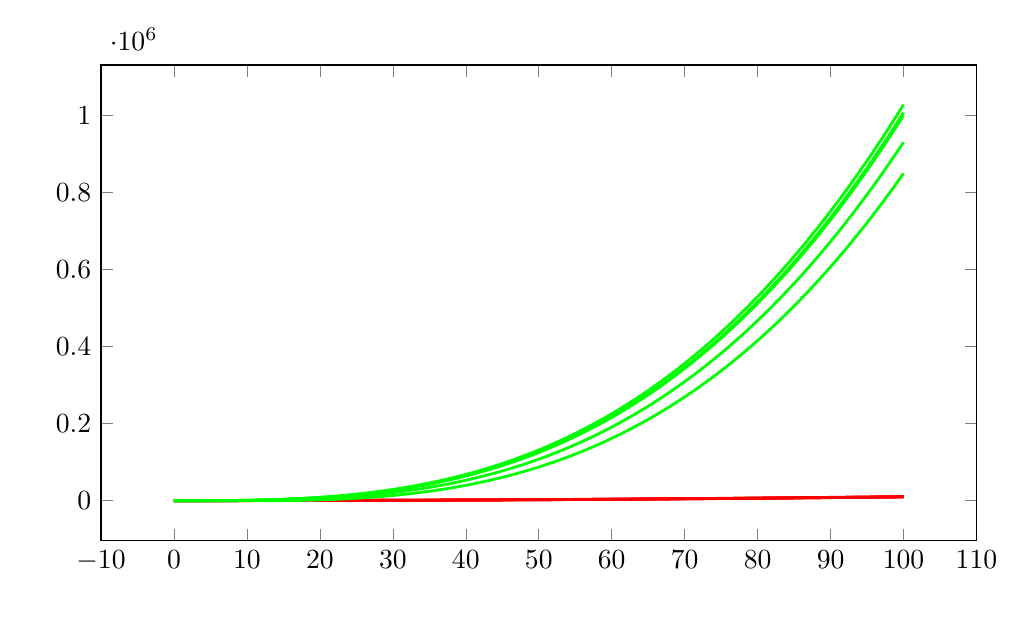
\begin{tikzpicture}[line width=1]
\begin{axis}[width=5in, height=3in,
             scatter/classes={a={mark=*,draw=black}},
             xlabel={\mbox{}},
             xlabel style={name=xlabel}, 
             ylabel={\mbox{}}, 
             legend style={
                at={(xlabel.south)},
                yshift=-1ex,
                anchor=north,
                legend cell align=left,
                },
        ]
]
\addplot[draw=red, line width=1] coordinates {(0.0,0.0)
(1.0101,1.0203)
(2.0202,4.0812)
(3.0303,9.1827)
(4.0404,16.3249)
(5.0505,25.5076)
(6.0606,36.7309)
(7.0707,49.9949)
(8.0808,65.2995)
(9.0909,82.6446)
(10.101,102.0304)
(11.1111,123.4568)
(12.1212,146.9238)
(13.1313,172.4314)
(14.1414,199.9796)
(15.1515,229.5684)
(16.1616,261.1978)
(17.1717,294.8679)
(18.1818,330.5785)
(19.1919,368.3298)
(20.202,408.1216)
(21.2121,449.9541)
(22.2222,493.8272)
(23.2323,539.7408)
(24.2424,587.6951)
(25.2525,637.69)
(26.2626,689.7255)
(27.2727,743.8017)
(28.2828,799.9184)
(29.2929,858.0757)
(30.303,918.2736)
(31.3131,980.5122)
(32.3232,1044.7913)
(33.3333,1111.1111)
(34.3434,1179.4715)
(35.3535,1249.8725)
(36.3636,1322.314)
(37.3737,1396.7962)
(38.3838,1473.319)
(39.3939,1551.8825)
(40.404,1632.4865)
(41.4141,1715.1311)
(42.4242,1799.8163)
(43.4343,1886.5422)
(44.4444,1975.3086)
(45.4545,2066.1157)
(46.4646,2158.9634)
(47.4747,2253.8516)
(48.4848,2350.7805)
(49.4949,2449.75)
(50.5051,2550.7601)
(51.5152,2653.8108)
(52.5253,2758.9022)
(53.5354,2866.0341)
(54.5455,2975.2066)
(55.5556,3086.4198)
(56.5657,3199.6735)
(57.5758,3314.9679)
(58.5859,3432.3028)
(59.596,3551.6784)
(60.6061,3673.0946)
(61.6162,3796.5514)
(62.6263,3922.0488)
(63.6364,4049.5868)
(64.6465,4179.1654)
(65.6566,4310.7846)
(66.6667,4444.4444)
(67.6768,4580.1449)
(68.6869,4717.8859)
(69.697,4857.6676)
(70.7071,4999.4898)
(71.7172,5143.3527)
(72.7273,5289.2562)
(73.7374,5437.2003)
(74.7475,5587.185)
(75.7576,5739.2103)
(76.7677,5893.2762)
(77.7778,6049.3827)
(78.7879,6207.5298)
(79.798,6367.7176)
(80.8081,6529.9459)
(81.8182,6694.2149)
(82.8283,6860.5244)
(83.8384,7028.8746)
(84.8485,7199.2654)
(85.8586,7371.6968)
(86.8687,7546.1688)
(87.8788,7722.6814)
(88.8889,7901.2346)
(89.899,8081.8284)
(90.9091,8264.4628)
(91.9192,8449.1378)
(92.9293,8635.8535)
(93.9394,8824.6097)
(94.9495,9015.4066)
(95.9596,9208.2441)
(96.9697,9403.1221)
(97.9798,9600.0408)
(98.9899,9799.0001)
(100.0,10000.0)};\addplot[draw=red, line width=1] coordinates {(0.0,2.0)
(1.0101,3.0203)
(2.0202,6.0812)
(3.0303,11.1827)
(4.0404,18.3249)
(5.0505,27.5076)
(6.0606,38.7309)
(7.0707,51.9949)
(8.0808,67.2995)
(9.0909,84.6446)
(10.101,104.0304)
(11.1111,125.4568)
(12.1212,148.9238)
(13.1313,174.4314)
(14.1414,201.9796)
(15.1515,231.5684)
(16.1616,263.1978)
(17.1717,296.8679)
(18.1818,332.5785)
(19.1919,370.3298)
(20.202,410.1216)
(21.2121,451.9541)
(22.2222,495.8272)
(23.2323,541.7408)
(24.2424,589.6951)
(25.2525,639.69)
(26.2626,691.7255)
(27.2727,745.8017)
(28.2828,801.9184)
(29.2929,860.0757)
(30.303,920.2736)
(31.3131,982.5122)
(32.3232,1046.7913)
(33.3333,1113.1111)
(34.3434,1181.4715)
(35.3535,1251.8725)
(36.3636,1324.314)
(37.3737,1398.7962)
(38.3838,1475.319)
(39.3939,1553.8825)
(40.404,1634.4865)
(41.4141,1717.1311)
(42.4242,1801.8163)
(43.4343,1888.5422)
(44.4444,1977.3086)
(45.4545,2068.1157)
(46.4646,2160.9634)
(47.4747,2255.8516)
(48.4848,2352.7805)
(49.4949,2451.75)
(50.5051,2552.7601)
(51.5152,2655.8108)
(52.5253,2760.9022)
(53.5354,2868.0341)
(54.5455,2977.2066)
(55.5556,3088.4198)
(56.5657,3201.6735)
(57.5758,3316.9679)
(58.5859,3434.3028)
(59.596,3553.6784)
(60.6061,3675.0946)
(61.6162,3798.5514)
(62.6263,3924.0488)
(63.6364,4051.5868)
(64.6465,4181.1654)
(65.6566,4312.7846)
(66.6667,4446.4444)
(67.6768,4582.1449)
(68.6869,4719.8859)
(69.697,4859.6676)
(70.7071,5001.4898)
(71.7172,5145.3527)
(72.7273,5291.2562)
(73.7374,5439.2003)
(74.7475,5589.185)
(75.7576,5741.2103)
(76.7677,5895.2762)
(77.7778,6051.3827)
(78.7879,6209.5298)
(79.798,6369.7176)
(80.8081,6531.9459)
(81.8182,6696.2149)
(82.8283,6862.5244)
(83.8384,7030.8746)
(84.8485,7201.2654)
(85.8586,7373.6968)
(86.8687,7548.1688)
(87.8788,7724.6814)
(88.8889,7903.2346)
(89.899,8083.8284)
(90.9091,8266.4628)
(91.9192,8451.1378)
(92.9293,8637.8535)
(93.9394,8826.6097)
(94.9495,9017.4066)
(95.9596,9210.2441)
(96.9697,9405.1221)
(97.9798,9602.0408)
(98.9899,9801.0001)
(100.0,10002.0)};\addplot[draw=red, line width=1] coordinates {(0.0,1.0)
(1.0101,2.0203)
(2.0202,5.0812)
(3.0303,10.1827)
(4.0404,17.3249)
(5.0505,26.5076)
(6.0606,37.7309)
(7.0707,50.9949)
(8.0808,66.2995)
(9.0909,83.6446)
(10.101,103.0304)
(11.1111,124.4568)
(12.1212,147.9238)
(13.1313,173.4314)
(14.1414,200.9796)
(15.1515,230.5684)
(16.1616,262.1978)
(17.1717,295.8679)
(18.1818,331.5785)
(19.1919,369.3298)
(20.202,409.1216)
(21.2121,450.9541)
(22.2222,494.8272)
(23.2323,540.7408)
(24.2424,588.6951)
(25.2525,638.69)
(26.2626,690.7255)
(27.2727,744.8017)
(28.2828,800.9184)
(29.2929,859.0757)
(30.303,919.2736)
(31.3131,981.5122)
(32.3232,1045.7913)
(33.3333,1112.1111)
(34.3434,1180.4715)
(35.3535,1250.8725)
(36.3636,1323.314)
(37.3737,1397.7962)
(38.3838,1474.319)
(39.3939,1552.8825)
(40.404,1633.4865)
(41.4141,1716.1311)
(42.4242,1800.8163)
(43.4343,1887.5422)
(44.4444,1976.3086)
(45.4545,2067.1157)
(46.4646,2159.9634)
(47.4747,2254.8516)
(48.4848,2351.7805)
(49.4949,2450.75)
(50.5051,2551.7601)
(51.5152,2654.8108)
(52.5253,2759.9022)
(53.5354,2867.0341)
(54.5455,2976.2066)
(55.5556,3087.4198)
(56.5657,3200.6735)
(57.5758,3315.9679)
(58.5859,3433.3028)
(59.596,3552.6784)
(60.6061,3674.0946)
(61.6162,3797.5514)
(62.6263,3923.0488)
(63.6364,4050.5868)
(64.6465,4180.1654)
(65.6566,4311.7846)
(66.6667,4445.4444)
(67.6768,4581.1449)
(68.6869,4718.8859)
(69.697,4858.6676)
(70.7071,5000.4898)
(71.7172,5144.3527)
(72.7273,5290.2562)
(73.7374,5438.2003)
(74.7475,5588.185)
(75.7576,5740.2103)
(76.7677,5894.2762)
(77.7778,6050.3827)
(78.7879,6208.5298)
(79.798,6368.7176)
(80.8081,6530.9459)
(81.8182,6695.2149)
(82.8283,6861.5244)
(83.8384,7029.8746)
(84.8485,7200.2654)
(85.8586,7372.6968)
(86.8687,7547.1688)
(87.8788,7723.6814)
(88.8889,7902.2346)
(89.899,8082.8284)
(90.9091,8265.4628)
(91.9192,8450.1378)
(92.9293,8636.8535)
(93.9394,8825.6097)
(94.9495,9016.4066)
(95.9596,9209.2441)
(96.9697,9404.1221)
(97.9798,9601.0408)
(98.9899,9800.0001)
(100.0,10001.0)};\addplot[draw=red, line width=1] coordinates {(0.0,-5.0)
(1.0101,1.0708)
(2.0202,9.1822)
(3.0303,19.3343)
(4.0404,31.5269)
(5.0505,45.7601)
(6.0606,62.034)
(7.0707,80.3484)
(8.0808,100.7035)
(9.0909,123.0992)
(10.101,147.5355)
(11.1111,174.0123)
(12.1212,202.5298)
(13.1313,233.088)
(14.1414,265.6867)
(15.1515,300.326)
(16.1616,337.0059)
(17.1717,375.7265)
(18.1818,416.4876)
(19.1919,459.2894)
(20.202,504.1317)
(21.2121,551.0147)
(22.2222,599.9383)
(23.2323,650.9025)
(24.2424,703.9073)
(25.2525,758.9527)
(26.2626,816.0387)
(27.2727,875.1653)
(28.2828,936.3325)
(29.2929,999.5404)
(30.303,1064.7888)
(31.3131,1132.0778)
(32.3232,1201.4075)
(33.3333,1272.7778)
(34.3434,1346.1887)
(35.3535,1421.6401)
(36.3636,1499.1322)
(37.3737,1578.6649)
(38.3838,1660.2382)
(39.3939,1743.8522)
(40.404,1829.5067)
(41.4141,1917.2018)
(42.4242,2006.9376)
(43.4343,2098.7139)
(44.4444,2192.5309)
(45.4545,2288.3884)
(46.4646,2386.2866)
(47.4747,2486.2254)
(48.4848,2588.2048)
(49.4949,2692.2248)
(50.5051,2798.2854)
(51.5152,2906.3866)
(52.5253,3016.5284)
(53.5354,3128.7108)
(54.5455,3242.9339)
(55.5556,3359.1975)
(56.5657,3477.5018)
(57.5758,3597.8466)
(58.5859,3720.2321)
(59.596,3844.6582)
(60.6061,3971.1249)
(61.6162,4099.6322)
(62.6263,4230.1801)
(63.6364,4362.7686)
(64.6465,4497.3977)
(65.6566,4634.0674)
(66.6667,4772.7778)
(67.6768,4913.5287)
(68.6869,5056.3203)
(69.697,5201.1524)
(70.7071,5348.0252)
(71.7172,5496.9386)
(72.7273,5647.8926)
(73.7374,5800.8872)
(74.7475,5955.9224)
(75.7576,6112.9982)
(76.7677,6272.1146)
(77.7778,6433.2716)
(78.7879,6596.4692)
(79.798,6761.7075)
(80.8081,6928.9863)
(81.8182,7098.3058)
(82.8283,7269.6659)
(83.8384,7443.0665)
(84.8485,7618.5078)
(85.8586,7795.9897)
(86.8687,7975.5122)
(87.8788,8157.0753)
(88.8889,8340.679)
(89.899,8526.3233)
(90.9091,8714.0083)
(91.9192,8903.7338)
(92.9293,9095.4999)
(93.9394,9289.3067)
(94.9495,9485.1541)
(95.9596,9683.042)
(96.9697,9882.9706)
(97.9798,10084.9398)
(98.9899,10288.9496)
(100.0,10495.0)};\addplot[draw=red, line width=1] coordinates {(0.0,-8.0)
(1.0101,-10.01)
(2.0202,-9.9794)
(3.0303,-7.9082)
(4.0404,-3.7963)
(5.0505,2.3561)
(6.0606,10.5491)
(7.0707,20.7828)
(8.0808,33.057)
(9.0909,47.3719)
(10.101,63.7274)
(11.1111,82.1235)
(12.1212,102.5601)
(13.1313,125.0374)
(14.1414,149.5554)
(15.1515,176.1139)
(16.1616,204.713)
(17.1717,235.3527)
(18.1818,268.0331)
(19.1919,302.754)
(20.202,339.5156)
(21.2121,378.3177)
(22.2222,419.1605)
(23.2323,462.0439)
(24.2424,506.9679)
(25.2525,553.9325)
(26.2626,602.9377)
(27.2727,653.9835)
(28.2828,707.0699)
(29.2929,762.1969)
(30.303,819.3646)
(31.3131,878.5728)
(32.3232,939.8217)
(33.3333,1003.1111)
(34.3434,1068.4412)
(35.3535,1135.8119)
(36.3636,1205.2231)
(37.3737,1276.675)
(38.3838,1350.1675)
(39.3939,1425.7006)
(40.404,1503.2744)
(41.4141,1582.8887)
(42.4242,1664.5436)
(43.4343,1748.2392)
(44.4444,1833.9753)
(45.4545,1921.7521)
(46.4646,2011.5694)
(47.4747,2103.4274)
(48.4848,2197.326)
(49.4949,2293.2652)
(50.5051,2391.245)
(51.5152,2491.2654)
(52.5253,2593.3264)
(53.5354,2697.428)
(54.5455,2803.5702)
(55.5556,2911.7531)
(56.5657,3021.9765)
(57.5758,3134.2406)
(58.5859,3248.5453)
(59.596,3364.8905)
(60.6061,3483.2764)
(61.6162,3603.7029)
(62.6263,3726.17)
(63.6364,3850.6777)
(64.6465,3977.226)
(65.6566,4105.8149)
(66.6667,4236.4444)
(67.6768,4369.1146)
(68.6869,4503.8253)
(69.697,4640.5767)
(70.7071,4779.3686)
(71.7172,4920.2012)
(72.7273,5063.0744)
(73.7374,5207.9882)
(74.7475,5354.9426)
(75.7576,5503.9376)
(76.7677,5654.9732)
(77.7778,5808.0494)
(78.7879,5963.1662)
(79.798,6120.3236)
(80.8081,6279.5217)
(81.8182,6440.7603)
(82.8283,6604.0396)
(83.8384,6769.3595)
(84.8485,6936.7199)
(85.8586,7106.121)
(86.8687,7277.5627)
(87.8788,7451.045)
(88.8889,7626.5679)
(89.899,7804.1314)
(90.9091,7983.7355)
(91.9192,8165.3803)
(92.9293,8349.0656)
(93.9394,8534.7916)
(94.9495,8722.5581)
(95.9596,8912.3653)
(96.9697,9104.213)
(97.9798,9298.1014)
(98.9899,9494.0304)
(100.0,9692.0)};\addplot[draw=green, line width=1] coordinates {(0.0,0.0)
(1.0101,1.0306)
(2.0202,8.2449)
(3.0303,27.8265)
(4.0404,65.959)
(5.0505,128.8263)
(6.0606,222.6118)
(7.0707,353.4993)
(8.0808,527.6724)
(9.0909,751.3148)
(10.101,1030.6102)
(11.1111,1371.7421)
(12.1212,1780.8943)
(13.1313,2264.2505)
(14.1414,2827.9943)
(15.1515,3478.3093)
(16.1616,4221.3792)
(17.1717,5063.3877)
(18.1818,6010.5184)
(19.1919,7068.955)
(20.202,8244.8812)
(21.2121,9544.4806)
(22.2222,10973.9369)
(23.2323,12539.4337)
(24.2424,14247.1547)
(25.2525,16103.2836)
(26.2626,18114.004)
(27.2727,20285.4996)
(28.2828,22623.9541)
(29.2929,25135.551)
(30.303,27826.4741)
(31.3131,30702.907)
(32.3232,33771.0335)
(33.3333,37037.037)
(34.3434,40507.1014)
(35.3535,44187.4103)
(36.3636,48084.1473)
(37.3737,52203.496)
(38.3838,56551.6403)
(39.3939,61134.7636)
(40.404,65959.0497)
(41.4141,71030.6823)
(42.4242,76355.845)
(43.4343,81940.7214)
(44.4444,87791.4952)
(45.4545,93914.3501)
(46.4646,100315.4698)
(47.4747,107001.0378)
(48.4848,113977.2379)
(49.4949,121250.2538)
(50.5051,128826.269)
(51.5152,136711.4673)
(52.5253,144912.0323)
(53.5354,153434.1476)
(54.5455,162283.997)
(55.5556,171467.7641)
(56.5657,180991.6325)
(57.5758,190861.7859)
(58.5859,201084.408)
(59.596,211665.6824)
(60.6061,222611.7929)
(61.6162,233928.9229)
(62.6263,245623.2563)
(63.6364,257700.9767)
(64.6465,270168.2677)
(65.6566,283031.313)
(66.6667,296296.2963)
(67.6768,309969.4012)
(68.6869,324056.8114)
(69.697,338564.7105)
(70.7071,353499.2822)
(71.7172,368866.7102)
(72.7273,384673.1781)
(73.7374,400924.8696)
(74.7475,417627.9683)
(75.7576,434788.6579)
(76.7677,452413.1221)
(77.7778,470507.5446)
(78.7879,489078.1089)
(79.798,508130.9988)
(80.8081,527672.3979)
(81.8182,547708.4899)
(82.8283,568245.4584)
(83.8384,589289.4871)
(84.8485,610846.7596)
(85.8586,632923.4597)
(86.8687,655525.7709)
(87.8788,678659.877)
(88.8889,702331.9616)
(89.899,726548.2083)
(90.9091,751314.8009)
(91.9192,776637.9229)
(92.9293,802523.7581)
(93.9394,828978.4901)
(94.9495,856008.3026)
(95.9596,883619.3792)
(96.9697,911817.9036)
(97.9798,940610.0594)
(98.9899,970002.0303)
(100.0,1000000.0)};\addplot[draw=green, line width=1] coordinates {(0.0,-5.0)
(1.0101,-21.1105)
(2.0202,-24.9155)
(3.0303,-10.2314)
(4.0404,29.1256)
(5.0505,99.339)
(6.0606,206.5925)
(7.0707,357.0698)
(8.0808,556.9546)
(9.0909,812.4305)
(10.101,1129.6812)
(11.1111,1514.8903)
(12.1212,1974.2415)
(13.1313,2513.9184)
(14.1414,3140.1048)
(15.1515,3858.9842)
(16.1616,4676.7404)
(17.1717,5599.5569)
(18.1818,6633.6176)
(19.1919,7785.1059)
(20.202,9060.2057)
(21.2121,10465.1005)
(22.2222,12005.9739)
(23.2323,13689.0098)
(24.2424,15520.3917)
(25.2525,17506.3032)
(26.2626,19652.9281)
(27.2727,21966.45)
(28.2828,24453.0526)
(29.2929,27118.9195)
(30.303,29970.2344)
(31.3131,33013.181)
(32.3232,36253.9429)
(33.3333,39698.7037)
(34.3434,43353.6472)
(35.3535,47224.957)
(36.3636,51318.8167)
(37.3737,55641.41)
(38.3838,60198.9206)
(39.3939,64997.5322)
(40.404,70043.4284)
(41.4141,75342.7928)
(42.4242,80901.8091)
(43.4343,86726.6611)
(44.4444,92823.5322)
(45.4545,99198.6063)
(46.4646,105858.067)
(47.4747,112808.0978)
(48.4848,120054.8826)
(49.4949,127604.6049)
(50.5051,135463.4484)
(51.5152,143637.5968)
(52.5253,152133.2337)
(53.5354,160956.5428)
(54.5455,170113.7077)
(55.5556,179610.9122)
(56.5657,189454.3399)
(57.5758,199650.1743)
(58.5859,210204.5993)
(59.596,221123.7984)
(60.6061,232413.9554)
(61.6162,244081.2538)
(62.6263,256131.8774)
(63.6364,268572.0098)
(64.6465,281407.8346)
(65.6566,294645.5356)
(66.6667,308291.2963)
(67.6768,322351.3005)
(68.6869,336831.7318)
(69.697,351738.7738)
(70.7071,367078.6103)
(71.7172,382857.4249)
(72.7273,399081.4012)
(73.7374,415756.7229)
(74.7475,432889.5737)
(75.7576,450486.1373)
(76.7677,468552.5972)
(77.7778,487095.1372)
(78.7879,506119.9409)
(79.798,525633.1919)
(80.8081,545641.074)
(81.8182,566149.7708)
(82.8283,587165.466)
(83.8384,608694.3432)
(84.8485,630742.5861)
(85.8586,653316.3783)
(86.8687,676421.9035)
(87.8788,700065.3453)
(88.8889,724252.8875)
(89.899,748990.7137)
(90.9091,774285.0075)
(91.9192,800141.9526)
(92.9293,826567.7327)
(93.9394,853568.5315)
(94.9495,881150.5325)
(95.9596,909319.9194)
(96.9697,938082.876)
(97.9798,967445.5859)
(98.9899,997414.2326)
(100.0,1027995.0)};\addplot[draw=green, line width=1] coordinates {(0.0,-15.0)
(1.0101,-38.2016)
(2.0202,-53.179)
(3.0303,-53.7484)
(4.0404,-33.7262)
(5.0505,13.0712)
(6.0606,92.8276)
(7.0707,211.7265)
(8.0808,375.9517)
(9.0909,591.6867)
(10.101,865.1153)
(11.1111,1202.4211)
(12.1212,1609.7878)
(13.1313,2093.3991)
(14.1414,2659.4385)
(15.1515,3314.0898)
(16.1616,4063.5366)
(17.1717,4913.9626)
(18.1818,5871.5515)
(19.1919,6942.4868)
(20.202,8132.9523)
(21.2121,9449.1317)
(22.2222,10897.2085)
(23.2323,12483.3665)
(24.2424,14213.7893)
(25.2525,16094.6605)
(26.2626,18132.1639)
(27.2727,20332.4831)
(28.2828,22701.8017)
(29.2929,25246.3035)
(30.303,27972.172)
(31.3131,30885.591)
(32.3232,33992.744)
(33.3333,37299.8148)
(34.3434,40812.987)
(35.3535,44538.4444)
(36.3636,48482.3704)
(37.3737,52650.9488)
(38.3838,57050.3634)
(39.3939,61686.7976)
(40.404,66566.4352)
(41.4141,71695.4599)
(42.4242,77080.0552)
(43.4343,82726.405)
(44.4444,88640.6927)
(45.4545,94829.1022)
(46.4646,101297.817)
(47.4747,108053.0208)
(48.4848,115100.8973)
(49.4949,122447.6301)
(50.5051,130099.4029)
(51.5152,138062.3993)
(52.5253,146342.8031)
(53.5354,154946.7979)
(54.5455,163880.5672)
(55.5556,173150.2949)
(56.5657,182762.1646)
(57.5758,192722.3598)
(58.5859,203037.0644)
(59.596,213712.4618)
(60.6061,224754.7359)
(61.6162,236170.0703)
(62.6263,247964.6485)
(63.6364,260144.6544)
(64.6465,272716.2715)
(65.6566,285685.6835)
(66.6667,299059.0741)
(67.6768,312842.6269)
(68.6869,327042.5256)
(69.697,341664.9538)
(70.7071,356716.0953)
(71.7172,372202.1336)
(72.7273,388129.2524)
(73.7374,404503.6355)
(74.7475,421331.4664)
(75.7576,438618.9288)
(76.7677,456372.2064)
(77.7778,474597.4829)
(78.7879,493300.9418)
(79.798,512488.7669)
(80.8081,532167.1418)
(81.8182,552342.2502)
(82.8283,573020.2757)
(83.8384,594207.4021)
(84.8485,615909.8129)
(85.8586,638133.6918)
(86.8687,660885.2225)
(87.8788,684170.5887)
(88.8889,707995.9739)
(89.899,732367.562)
(90.9091,757291.5364)
(91.9192,782774.081)
(92.9293,808821.3793)
(93.9394,835439.615)
(94.9495,862634.9718)
(95.9596,890413.6333)
(96.9697,918781.7833)
(97.9798,947745.6052)
(98.9899,977311.2829)
(100.0,1007485.0)};\addplot[draw=green, line width=1] coordinates {(0.0,1.0)
(1.0101,-18.3245)
(2.0202,-62.0744)
(3.0303,-124.0661)
(4.0404,-198.1159)
(5.0505,-278.0403)
(6.0606,-357.6554)
(7.0707,-430.7777)
(8.0808,-491.2235)
(9.0909,-532.8092)
(10.101,-549.351)
(11.1111,-534.6653)
(12.1212,-482.5685)
(13.1313,-386.8768)
(14.1414,-241.4067)
(15.1515,-39.9745)
(16.1616,223.6035)
(17.1717,555.511)
(18.1818,961.9316)
(19.1919,1449.049)
(20.202,2023.0468)
(21.2121,2690.1087)
(22.2222,3456.4184)
(23.2323,4328.1595)
(24.2424,5311.5156)
(25.2525,6412.6705)
(26.2626,7637.8078)
(27.2727,8993.1112)
(28.2828,10484.7643)
(29.2929,12118.9508)
(30.303,13901.8543)
(31.3131,15839.6585)
(32.3232,17938.5471)
(33.3333,20204.7037)
(34.3434,22644.312)
(35.3535,25263.5557)
(36.3636,28068.6183)
(37.3737,31065.6837)
(38.3838,34260.9353)
(39.3939,37660.557)
(40.404,41270.7323)
(41.4141,45097.645)
(42.4242,49147.4786)
(43.4343,53426.4168)
(44.4444,57940.6433)
(45.4545,62696.3418)
(46.4646,67699.696)
(47.4747,72956.8894)
(48.4848,78474.1057)
(49.4949,84257.5287)
(50.5051,90313.3419)
(51.5152,96647.729)
(52.5253,103266.8737)
(53.5354,110176.9597)
(54.5455,117384.1705)
(55.5556,124894.69)
(56.5657,132714.7017)
(57.5758,140850.3892)
(58.5859,149307.9363)
(59.596,158093.5266)
(60.6061,167213.3438)
(61.6162,176673.5715)
(62.6263,186480.3935)
(63.6364,196639.9932)
(64.6465,207158.5545)
(65.6566,218042.261)
(66.6667,229297.2963)
(67.6768,240929.8441)
(68.6869,252946.0881)
(69.697,265352.2118)
(70.7071,278154.3991)
(71.7172,291358.8335)
(72.7273,304971.6987)
(73.7374,318999.1784)
(74.7475,333447.4562)
(75.7576,348322.7158)
(76.7677,363631.1408)
(77.7778,379378.915)
(78.7879,395572.2219)
(79.798,412217.2452)
(80.8081,429320.1686)
(81.8182,446887.1758)
(82.8283,464924.4504)
(83.8384,483438.1761)
(84.8485,502434.5365)
(85.8586,521919.7153)
(86.8687,541899.8961)
(87.8788,562381.2627)
(88.8889,583369.9986)
(89.899,604872.2876)
(90.9091,626894.3133)
(91.9192,649442.2593)
(92.9293,672522.3094)
(93.9394,696140.6472)
(94.9495,720303.4563)
(95.9596,745016.9204)
(96.9697,770287.2231)
(97.9798,796120.5482)
(98.9899,822523.0793)
(100.0,849501.0)};\addplot[draw=green, line width=1] coordinates {(0.0,-100.0)
(1.0101,-101.061)
(2.0202,-110.2226)
(3.0303,-121.3012)
(4.0404,-128.113)
(5.0505,-124.4744)
(6.0606,-104.2018)
(7.0707,-61.1115)
(8.0808,10.9802)
(9.0909,118.2569)
(10.101,266.9024)
(11.1111,463.1001)
(12.1212,713.0339)
(13.1313,1022.8874)
(14.1414,1398.8442)
(15.1515,1847.088)
(16.1616,2373.8024)
(17.1717,2985.1712)
(18.1818,3687.3779)
(19.1919,4486.6063)
(20.202,5389.04)
(21.2121,6400.8626)
(22.2222,7528.2579)
(23.2323,8777.4094)
(24.2424,10154.5009)
(25.2525,11665.716)
(26.2626,13317.2384)
(27.2727,15115.2517)
(28.2828,17065.9396)
(29.2929,19175.4857)
(30.303,21450.0737)
(31.3131,23895.8874)
(32.3232,26519.1102)
(33.3333,29325.9259)
(34.3434,32322.5182)
(35.3535,35515.0707)
(36.3636,38909.7671)
(37.3737,42512.791)
(38.3838,46330.3261)
(39.3939,50368.5561)
(40.404,54633.6646)
(41.4141,59131.8352)
(42.4242,63869.2517)
(43.4343,68852.0978)
(44.4444,74086.5569)
(45.4545,79578.8129)
(46.4646,85335.0494)
(47.4747,91361.45)
(48.4848,97664.1985)
(49.4949,104249.4784)
(50.5051,111123.4734)
(51.5152,118292.3672)
(52.5253,125762.3435)
(53.5354,133539.5858)
(54.5455,141630.278)
(55.5556,150040.6036)
(56.5657,158776.7462)
(57.5758,167844.8897)
(58.5859,177251.2175)
(59.596,187001.9134)
(60.6061,197103.1611)
(61.6162,207561.1441)
(62.6263,218382.0463)
(63.6364,229572.0511)
(64.6465,241137.3423)
(65.6566,253084.1036)
(66.6667,265418.5185)
(67.6768,278146.7708)
(68.6869,291275.0442)
(69.697,304809.5222)
(70.7071,318756.3886)
(71.7172,333121.827)
(72.7273,347912.021)
(73.7374,363133.1544)
(74.7475,378791.4108)
(75.7576,394892.9738)
(76.7677,411444.0272)
(77.7778,428450.7545)
(78.7879,445919.3394)
(79.798,463855.9656)
(80.8081,482266.8168)
(81.8182,501158.0766)
(82.8283,520535.9287)
(83.8384,540406.5567)
(84.8485,560776.1444)
(85.8586,581650.8752)
(86.8687,603036.933)
(87.8788,624940.5014)
(88.8889,647367.7641)
(89.899,670324.9046)
(90.9091,693818.1067)
(91.9192,717853.554)
(92.9293,742437.4302)
(93.9394,767575.919)
(94.9495,793275.2039)
(95.9596,819541.4688)
(96.9697,846380.8971)
(97.9798,873799.6727)
(98.9899,901803.9791)
(100.0,930400.0)};
\end{axis}\end{tikzpicture}\end{center}


The five functions which are higher up are:
\begin{align*}
&n^3 \\
&n^3 + 3n^2 - 20n - 5 \\
&n^3 +   n^2 - 25n - 15 \\
&n^3 - 15n^2 - 5n + 1 \\
&n^3 - 7n^2 + 5n - 100
\end{align*}
and the last group of five functions are:
\begin{align*}
&n^2 \\
&n^2 + 2 \\
&n^2 + 1 \\
&n^2 + 5n - 5 \\
&n^2 - 3n - 8
\end{align*}

As you can see, in terms of growth, for large values of $n$, the 15 functions
\begin{align*}
&n^4 \\
&n^4 + n^2 - 20n - 9 \\
&n^4 +  n^3 - 25n - 1 \\
&n^4 - 15x^2 - 5n + 1 \\
&n^4 - 2x^2 - 7m - 100 \\
&n^3 \\
&n^3 + 3n^2 - 20n - 5 \\
&n^3 +   n^2 - 25n - 15 \\
&n^3 - 15n^2 - 5n + 1 \\
&n^3 - 7n^2 + 5n - 100 \\
&n^2 \\
&n^2 + 2 \\
&n^2 + 1 \\
&n^2 + 5n - 5 \\
&n^2 - 3n - 8
\end{align*}
bunches themselves up into 3 groups determined by their degrees.
You can think of the following as leaders in the three groups:
\begin{align*}
&n^4 \\
&n^3 \\
&n^2
\end{align*}
(because they are the simplest.)

In general \textit{all} polynomial functions with 1 for the leading coefficient -- such polynomials
are said to be \defterm{monic} polynomials -- 
group themselves up into
bunches led by the following leaders:
\[
1, \,\,\,\,\,
n, \,\,\,\,\,
n^2, \,\,\,\,\,
n^3, \,\,\,\,\,
n^4, \,\,\,\,\,
n^5, \,\,\,\,\,
n^6, \,\,\,\,\,
\ldots
\]
The bunching up for large $n$ is due to the fact that they grow (or climb) at the same rate for large $n$.
This means that the function
\[
n^2 - 42n + 691
\]
has the same growth rate as $n^2$ for large $n$.
Graphically, this means that when you zoom out (i.e., when you draw their graph for a
large domain), the graphs collapse into one.
Intuitively, you can think of it this way:
\[
\text{$n^2 - 42n + 691$ \lq\lq roughly $=$" $n^2$ \,\,\,\,\ for large $n$}
\]

Now let's get back to big-O.
Whereas the above examples talked about 
\[
\text{... \lq\lq roughly $=$'' ... \,\,\,\,\, for large $n$}
\]
big-O is more like
\[
\text{... \lq\lq roughly $\leq$'' ... \,\,\,\,\, for large $n$}
\]
Graphically, if the graph of $f(n)$ is \textit{below} the graph to $g(n)$
\textit{for large $n$}, then we can say
\[
f(n) = O(g(n))
\]
Now, one of the above 15 functions is this:
\[
n^3 + 3n^2 - 20n - 5
\]
We have already seen that the graph of 
$n^3 + 3n^2 - 20n - 5$
is the same as the graph of $n^3$ for large $n$. 
I can say
\[
n^3 + 3n^2 - 20n - 5 = O(n^3)
\]
\textit{But, there's more.}
The graph of $n^3 + 3n^2 - 20n - 5$ is roughly the graph of $n^3$
(for large $n$) and 
is of course the graph of $n^3$ is below the graph of $n^4$.
Therefore the graph of 
$n^3 + 3n^2 - 20n - 5$
is roughly below the graph of $n^4$ (for large $n$).
Therefore I can also say
\[
n^3 + 3n^2 - 20n - 5 = O(n^4)
\]
Altogether I have
\begin{align*}
n^3 + 3n^2 - 20n - 5 &= O(n^3) \\
n^3 + 3n^2 - 20n - 5 &= O(n^4)
\end{align*}
It is also true that
\begin{align*}
n^3 + 3n^2 - 20n - 5 &= O(n^3 + 1) \\
n^3 + 3n^2 - 20n - 5 &= O(n^4 + 1)
\end{align*}

OK, let's try another function.
Here's another function from the 15:
\[
n^2 + 5n - 5
\]
Using the same reasoning we have all the following:
\begin{align*}
n^2 + 5n - 5 &= O(n^2) \\
n^2 + 5n - 5 &= O(n^3) \\
n^2 + 5n - 5 &= O(n^4)
\end{align*}


But there's a little bit more to big-O.
What about multiples of the above functions?
Recall that in the previous section,
I said that you should ignore multiples by replacing constants with 1.
It seems to mean that constants don't determine function growth rate.
Is that true?

Here are the original 15 functions again:
\begin{align*}
&n^4 \\
&n^4 + n^2 - 20n - 9 \\
&n^4 +  n^3 - 25n - 1 \\
&n^4 - 15x^2 - 5n + 1 \\
&n^4 - 2x^2 - 7m - 100 \\
&n^3 \\
&n^3 + 3n^2 - 20n - 5 \\
&n^3 +   n^2 - 25n - 15 \\
&n^3 - 15n^2 - 5n + 1 \\
&n^3 - 7n^2 + 5n - 100 \\
&n^2 \\
&n^2 + 2 \\
&n^2 + 1 \\
&n^2 + 5n - 5 \\
&n^2 - 3n - 8
\end{align*}
and now I'm going change the leading coefficients
\begin{align*}
&n^4 \\
&2n^4 + n^2 - 20n - 9 \\
&3n^4 +  n^3 - 25n - 1 \\
&4n^4 - 15x^2 - 5n + 1 \\
&5n^4 - 2x^2 - 7m - 100 \\
&6n^3 \\
&7n^3 + 3n^2 - 20n - 5 \\
&8n^3 +   n^2 - 25n - 15 \\
&9n^3 - 15n^2 - 5n + 1 \\
&10n^3 - 7n^2 + 5n - 100 \\
&11n^2 \\
&12n^2 + 2 \\
&13n^2 + 1 \\
&14n^2 + 5n - 5 \\
&15n^2 - 3n - 8
\end{align*}
and then plot the new functions on the domain $0 \leq n \leq 100$:
%-*-latex-*-

\begin{center}
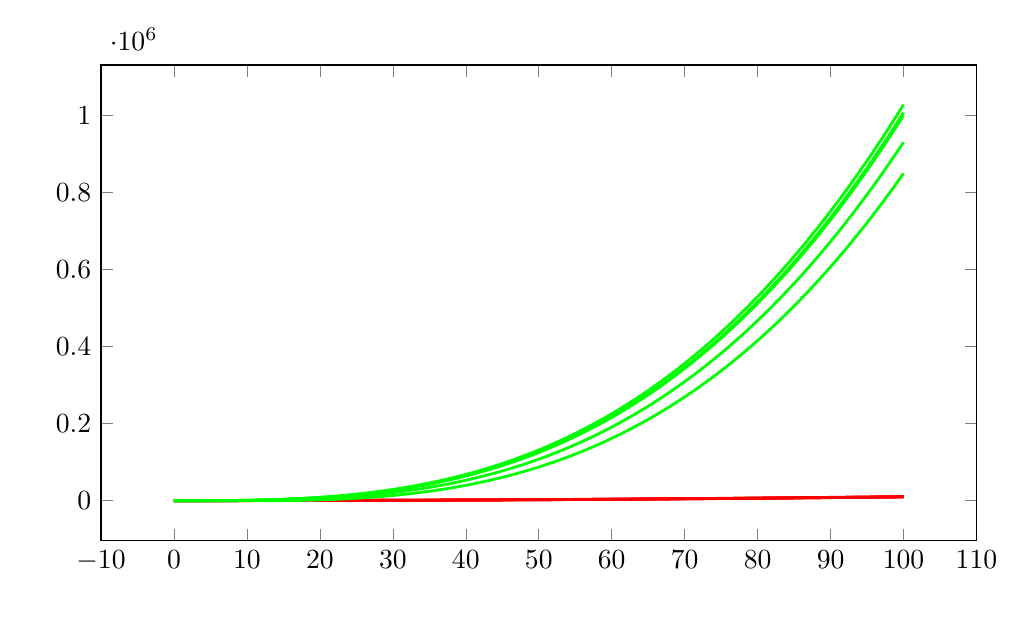
\begin{tikzpicture}[line width=1]
\begin{axis}[width=5in, height=3in,
             scatter/classes={a={mark=*,draw=black}},
             xlabel={\mbox{}},
             xlabel style={name=xlabel}, 
             ylabel={\mbox{}}, 
             legend style={
                at={(xlabel.south)},
                yshift=-1ex,
                anchor=north,
                legend cell align=left,
                },
        ]
]
\addplot[draw=red, line width=1] coordinates {(0.0,0.0)
(1.0101,1.0203)
(2.0202,4.0812)
(3.0303,9.1827)
(4.0404,16.3249)
(5.0505,25.5076)
(6.0606,36.7309)
(7.0707,49.9949)
(8.0808,65.2995)
(9.0909,82.6446)
(10.101,102.0304)
(11.1111,123.4568)
(12.1212,146.9238)
(13.1313,172.4314)
(14.1414,199.9796)
(15.1515,229.5684)
(16.1616,261.1978)
(17.1717,294.8679)
(18.1818,330.5785)
(19.1919,368.3298)
(20.202,408.1216)
(21.2121,449.9541)
(22.2222,493.8272)
(23.2323,539.7408)
(24.2424,587.6951)
(25.2525,637.69)
(26.2626,689.7255)
(27.2727,743.8017)
(28.2828,799.9184)
(29.2929,858.0757)
(30.303,918.2736)
(31.3131,980.5122)
(32.3232,1044.7913)
(33.3333,1111.1111)
(34.3434,1179.4715)
(35.3535,1249.8725)
(36.3636,1322.314)
(37.3737,1396.7962)
(38.3838,1473.319)
(39.3939,1551.8825)
(40.404,1632.4865)
(41.4141,1715.1311)
(42.4242,1799.8163)
(43.4343,1886.5422)
(44.4444,1975.3086)
(45.4545,2066.1157)
(46.4646,2158.9634)
(47.4747,2253.8516)
(48.4848,2350.7805)
(49.4949,2449.75)
(50.5051,2550.7601)
(51.5152,2653.8108)
(52.5253,2758.9022)
(53.5354,2866.0341)
(54.5455,2975.2066)
(55.5556,3086.4198)
(56.5657,3199.6735)
(57.5758,3314.9679)
(58.5859,3432.3028)
(59.596,3551.6784)
(60.6061,3673.0946)
(61.6162,3796.5514)
(62.6263,3922.0488)
(63.6364,4049.5868)
(64.6465,4179.1654)
(65.6566,4310.7846)
(66.6667,4444.4444)
(67.6768,4580.1449)
(68.6869,4717.8859)
(69.697,4857.6676)
(70.7071,4999.4898)
(71.7172,5143.3527)
(72.7273,5289.2562)
(73.7374,5437.2003)
(74.7475,5587.185)
(75.7576,5739.2103)
(76.7677,5893.2762)
(77.7778,6049.3827)
(78.7879,6207.5298)
(79.798,6367.7176)
(80.8081,6529.9459)
(81.8182,6694.2149)
(82.8283,6860.5244)
(83.8384,7028.8746)
(84.8485,7199.2654)
(85.8586,7371.6968)
(86.8687,7546.1688)
(87.8788,7722.6814)
(88.8889,7901.2346)
(89.899,8081.8284)
(90.9091,8264.4628)
(91.9192,8449.1378)
(92.9293,8635.8535)
(93.9394,8824.6097)
(94.9495,9015.4066)
(95.9596,9208.2441)
(96.9697,9403.1221)
(97.9798,9600.0408)
(98.9899,9799.0001)
(100.0,10000.0)};\addplot[draw=red, line width=1] coordinates {(0.0,2.0)
(1.0101,3.0203)
(2.0202,6.0812)
(3.0303,11.1827)
(4.0404,18.3249)
(5.0505,27.5076)
(6.0606,38.7309)
(7.0707,51.9949)
(8.0808,67.2995)
(9.0909,84.6446)
(10.101,104.0304)
(11.1111,125.4568)
(12.1212,148.9238)
(13.1313,174.4314)
(14.1414,201.9796)
(15.1515,231.5684)
(16.1616,263.1978)
(17.1717,296.8679)
(18.1818,332.5785)
(19.1919,370.3298)
(20.202,410.1216)
(21.2121,451.9541)
(22.2222,495.8272)
(23.2323,541.7408)
(24.2424,589.6951)
(25.2525,639.69)
(26.2626,691.7255)
(27.2727,745.8017)
(28.2828,801.9184)
(29.2929,860.0757)
(30.303,920.2736)
(31.3131,982.5122)
(32.3232,1046.7913)
(33.3333,1113.1111)
(34.3434,1181.4715)
(35.3535,1251.8725)
(36.3636,1324.314)
(37.3737,1398.7962)
(38.3838,1475.319)
(39.3939,1553.8825)
(40.404,1634.4865)
(41.4141,1717.1311)
(42.4242,1801.8163)
(43.4343,1888.5422)
(44.4444,1977.3086)
(45.4545,2068.1157)
(46.4646,2160.9634)
(47.4747,2255.8516)
(48.4848,2352.7805)
(49.4949,2451.75)
(50.5051,2552.7601)
(51.5152,2655.8108)
(52.5253,2760.9022)
(53.5354,2868.0341)
(54.5455,2977.2066)
(55.5556,3088.4198)
(56.5657,3201.6735)
(57.5758,3316.9679)
(58.5859,3434.3028)
(59.596,3553.6784)
(60.6061,3675.0946)
(61.6162,3798.5514)
(62.6263,3924.0488)
(63.6364,4051.5868)
(64.6465,4181.1654)
(65.6566,4312.7846)
(66.6667,4446.4444)
(67.6768,4582.1449)
(68.6869,4719.8859)
(69.697,4859.6676)
(70.7071,5001.4898)
(71.7172,5145.3527)
(72.7273,5291.2562)
(73.7374,5439.2003)
(74.7475,5589.185)
(75.7576,5741.2103)
(76.7677,5895.2762)
(77.7778,6051.3827)
(78.7879,6209.5298)
(79.798,6369.7176)
(80.8081,6531.9459)
(81.8182,6696.2149)
(82.8283,6862.5244)
(83.8384,7030.8746)
(84.8485,7201.2654)
(85.8586,7373.6968)
(86.8687,7548.1688)
(87.8788,7724.6814)
(88.8889,7903.2346)
(89.899,8083.8284)
(90.9091,8266.4628)
(91.9192,8451.1378)
(92.9293,8637.8535)
(93.9394,8826.6097)
(94.9495,9017.4066)
(95.9596,9210.2441)
(96.9697,9405.1221)
(97.9798,9602.0408)
(98.9899,9801.0001)
(100.0,10002.0)};\addplot[draw=red, line width=1] coordinates {(0.0,1.0)
(1.0101,2.0203)
(2.0202,5.0812)
(3.0303,10.1827)
(4.0404,17.3249)
(5.0505,26.5076)
(6.0606,37.7309)
(7.0707,50.9949)
(8.0808,66.2995)
(9.0909,83.6446)
(10.101,103.0304)
(11.1111,124.4568)
(12.1212,147.9238)
(13.1313,173.4314)
(14.1414,200.9796)
(15.1515,230.5684)
(16.1616,262.1978)
(17.1717,295.8679)
(18.1818,331.5785)
(19.1919,369.3298)
(20.202,409.1216)
(21.2121,450.9541)
(22.2222,494.8272)
(23.2323,540.7408)
(24.2424,588.6951)
(25.2525,638.69)
(26.2626,690.7255)
(27.2727,744.8017)
(28.2828,800.9184)
(29.2929,859.0757)
(30.303,919.2736)
(31.3131,981.5122)
(32.3232,1045.7913)
(33.3333,1112.1111)
(34.3434,1180.4715)
(35.3535,1250.8725)
(36.3636,1323.314)
(37.3737,1397.7962)
(38.3838,1474.319)
(39.3939,1552.8825)
(40.404,1633.4865)
(41.4141,1716.1311)
(42.4242,1800.8163)
(43.4343,1887.5422)
(44.4444,1976.3086)
(45.4545,2067.1157)
(46.4646,2159.9634)
(47.4747,2254.8516)
(48.4848,2351.7805)
(49.4949,2450.75)
(50.5051,2551.7601)
(51.5152,2654.8108)
(52.5253,2759.9022)
(53.5354,2867.0341)
(54.5455,2976.2066)
(55.5556,3087.4198)
(56.5657,3200.6735)
(57.5758,3315.9679)
(58.5859,3433.3028)
(59.596,3552.6784)
(60.6061,3674.0946)
(61.6162,3797.5514)
(62.6263,3923.0488)
(63.6364,4050.5868)
(64.6465,4180.1654)
(65.6566,4311.7846)
(66.6667,4445.4444)
(67.6768,4581.1449)
(68.6869,4718.8859)
(69.697,4858.6676)
(70.7071,5000.4898)
(71.7172,5144.3527)
(72.7273,5290.2562)
(73.7374,5438.2003)
(74.7475,5588.185)
(75.7576,5740.2103)
(76.7677,5894.2762)
(77.7778,6050.3827)
(78.7879,6208.5298)
(79.798,6368.7176)
(80.8081,6530.9459)
(81.8182,6695.2149)
(82.8283,6861.5244)
(83.8384,7029.8746)
(84.8485,7200.2654)
(85.8586,7372.6968)
(86.8687,7547.1688)
(87.8788,7723.6814)
(88.8889,7902.2346)
(89.899,8082.8284)
(90.9091,8265.4628)
(91.9192,8450.1378)
(92.9293,8636.8535)
(93.9394,8825.6097)
(94.9495,9016.4066)
(95.9596,9209.2441)
(96.9697,9404.1221)
(97.9798,9601.0408)
(98.9899,9800.0001)
(100.0,10001.0)};\addplot[draw=red, line width=1] coordinates {(0.0,-5.0)
(1.0101,1.0708)
(2.0202,9.1822)
(3.0303,19.3343)
(4.0404,31.5269)
(5.0505,45.7601)
(6.0606,62.034)
(7.0707,80.3484)
(8.0808,100.7035)
(9.0909,123.0992)
(10.101,147.5355)
(11.1111,174.0123)
(12.1212,202.5298)
(13.1313,233.088)
(14.1414,265.6867)
(15.1515,300.326)
(16.1616,337.0059)
(17.1717,375.7265)
(18.1818,416.4876)
(19.1919,459.2894)
(20.202,504.1317)
(21.2121,551.0147)
(22.2222,599.9383)
(23.2323,650.9025)
(24.2424,703.9073)
(25.2525,758.9527)
(26.2626,816.0387)
(27.2727,875.1653)
(28.2828,936.3325)
(29.2929,999.5404)
(30.303,1064.7888)
(31.3131,1132.0778)
(32.3232,1201.4075)
(33.3333,1272.7778)
(34.3434,1346.1887)
(35.3535,1421.6401)
(36.3636,1499.1322)
(37.3737,1578.6649)
(38.3838,1660.2382)
(39.3939,1743.8522)
(40.404,1829.5067)
(41.4141,1917.2018)
(42.4242,2006.9376)
(43.4343,2098.7139)
(44.4444,2192.5309)
(45.4545,2288.3884)
(46.4646,2386.2866)
(47.4747,2486.2254)
(48.4848,2588.2048)
(49.4949,2692.2248)
(50.5051,2798.2854)
(51.5152,2906.3866)
(52.5253,3016.5284)
(53.5354,3128.7108)
(54.5455,3242.9339)
(55.5556,3359.1975)
(56.5657,3477.5018)
(57.5758,3597.8466)
(58.5859,3720.2321)
(59.596,3844.6582)
(60.6061,3971.1249)
(61.6162,4099.6322)
(62.6263,4230.1801)
(63.6364,4362.7686)
(64.6465,4497.3977)
(65.6566,4634.0674)
(66.6667,4772.7778)
(67.6768,4913.5287)
(68.6869,5056.3203)
(69.697,5201.1524)
(70.7071,5348.0252)
(71.7172,5496.9386)
(72.7273,5647.8926)
(73.7374,5800.8872)
(74.7475,5955.9224)
(75.7576,6112.9982)
(76.7677,6272.1146)
(77.7778,6433.2716)
(78.7879,6596.4692)
(79.798,6761.7075)
(80.8081,6928.9863)
(81.8182,7098.3058)
(82.8283,7269.6659)
(83.8384,7443.0665)
(84.8485,7618.5078)
(85.8586,7795.9897)
(86.8687,7975.5122)
(87.8788,8157.0753)
(88.8889,8340.679)
(89.899,8526.3233)
(90.9091,8714.0083)
(91.9192,8903.7338)
(92.9293,9095.4999)
(93.9394,9289.3067)
(94.9495,9485.1541)
(95.9596,9683.042)
(96.9697,9882.9706)
(97.9798,10084.9398)
(98.9899,10288.9496)
(100.0,10495.0)};\addplot[draw=red, line width=1] coordinates {(0.0,-8.0)
(1.0101,-10.01)
(2.0202,-9.9794)
(3.0303,-7.9082)
(4.0404,-3.7963)
(5.0505,2.3561)
(6.0606,10.5491)
(7.0707,20.7828)
(8.0808,33.057)
(9.0909,47.3719)
(10.101,63.7274)
(11.1111,82.1235)
(12.1212,102.5601)
(13.1313,125.0374)
(14.1414,149.5554)
(15.1515,176.1139)
(16.1616,204.713)
(17.1717,235.3527)
(18.1818,268.0331)
(19.1919,302.754)
(20.202,339.5156)
(21.2121,378.3177)
(22.2222,419.1605)
(23.2323,462.0439)
(24.2424,506.9679)
(25.2525,553.9325)
(26.2626,602.9377)
(27.2727,653.9835)
(28.2828,707.0699)
(29.2929,762.1969)
(30.303,819.3646)
(31.3131,878.5728)
(32.3232,939.8217)
(33.3333,1003.1111)
(34.3434,1068.4412)
(35.3535,1135.8119)
(36.3636,1205.2231)
(37.3737,1276.675)
(38.3838,1350.1675)
(39.3939,1425.7006)
(40.404,1503.2744)
(41.4141,1582.8887)
(42.4242,1664.5436)
(43.4343,1748.2392)
(44.4444,1833.9753)
(45.4545,1921.7521)
(46.4646,2011.5694)
(47.4747,2103.4274)
(48.4848,2197.326)
(49.4949,2293.2652)
(50.5051,2391.245)
(51.5152,2491.2654)
(52.5253,2593.3264)
(53.5354,2697.428)
(54.5455,2803.5702)
(55.5556,2911.7531)
(56.5657,3021.9765)
(57.5758,3134.2406)
(58.5859,3248.5453)
(59.596,3364.8905)
(60.6061,3483.2764)
(61.6162,3603.7029)
(62.6263,3726.17)
(63.6364,3850.6777)
(64.6465,3977.226)
(65.6566,4105.8149)
(66.6667,4236.4444)
(67.6768,4369.1146)
(68.6869,4503.8253)
(69.697,4640.5767)
(70.7071,4779.3686)
(71.7172,4920.2012)
(72.7273,5063.0744)
(73.7374,5207.9882)
(74.7475,5354.9426)
(75.7576,5503.9376)
(76.7677,5654.9732)
(77.7778,5808.0494)
(78.7879,5963.1662)
(79.798,6120.3236)
(80.8081,6279.5217)
(81.8182,6440.7603)
(82.8283,6604.0396)
(83.8384,6769.3595)
(84.8485,6936.7199)
(85.8586,7106.121)
(86.8687,7277.5627)
(87.8788,7451.045)
(88.8889,7626.5679)
(89.899,7804.1314)
(90.9091,7983.7355)
(91.9192,8165.3803)
(92.9293,8349.0656)
(93.9394,8534.7916)
(94.9495,8722.5581)
(95.9596,8912.3653)
(96.9697,9104.213)
(97.9798,9298.1014)
(98.9899,9494.0304)
(100.0,9692.0)};\addplot[draw=green, line width=1] coordinates {(0.0,0.0)
(1.0101,1.0306)
(2.0202,8.2449)
(3.0303,27.8265)
(4.0404,65.959)
(5.0505,128.8263)
(6.0606,222.6118)
(7.0707,353.4993)
(8.0808,527.6724)
(9.0909,751.3148)
(10.101,1030.6102)
(11.1111,1371.7421)
(12.1212,1780.8943)
(13.1313,2264.2505)
(14.1414,2827.9943)
(15.1515,3478.3093)
(16.1616,4221.3792)
(17.1717,5063.3877)
(18.1818,6010.5184)
(19.1919,7068.955)
(20.202,8244.8812)
(21.2121,9544.4806)
(22.2222,10973.9369)
(23.2323,12539.4337)
(24.2424,14247.1547)
(25.2525,16103.2836)
(26.2626,18114.004)
(27.2727,20285.4996)
(28.2828,22623.9541)
(29.2929,25135.551)
(30.303,27826.4741)
(31.3131,30702.907)
(32.3232,33771.0335)
(33.3333,37037.037)
(34.3434,40507.1014)
(35.3535,44187.4103)
(36.3636,48084.1473)
(37.3737,52203.496)
(38.3838,56551.6403)
(39.3939,61134.7636)
(40.404,65959.0497)
(41.4141,71030.6823)
(42.4242,76355.845)
(43.4343,81940.7214)
(44.4444,87791.4952)
(45.4545,93914.3501)
(46.4646,100315.4698)
(47.4747,107001.0378)
(48.4848,113977.2379)
(49.4949,121250.2538)
(50.5051,128826.269)
(51.5152,136711.4673)
(52.5253,144912.0323)
(53.5354,153434.1476)
(54.5455,162283.997)
(55.5556,171467.7641)
(56.5657,180991.6325)
(57.5758,190861.7859)
(58.5859,201084.408)
(59.596,211665.6824)
(60.6061,222611.7929)
(61.6162,233928.9229)
(62.6263,245623.2563)
(63.6364,257700.9767)
(64.6465,270168.2677)
(65.6566,283031.313)
(66.6667,296296.2963)
(67.6768,309969.4012)
(68.6869,324056.8114)
(69.697,338564.7105)
(70.7071,353499.2822)
(71.7172,368866.7102)
(72.7273,384673.1781)
(73.7374,400924.8696)
(74.7475,417627.9683)
(75.7576,434788.6579)
(76.7677,452413.1221)
(77.7778,470507.5446)
(78.7879,489078.1089)
(79.798,508130.9988)
(80.8081,527672.3979)
(81.8182,547708.4899)
(82.8283,568245.4584)
(83.8384,589289.4871)
(84.8485,610846.7596)
(85.8586,632923.4597)
(86.8687,655525.7709)
(87.8788,678659.877)
(88.8889,702331.9616)
(89.899,726548.2083)
(90.9091,751314.8009)
(91.9192,776637.9229)
(92.9293,802523.7581)
(93.9394,828978.4901)
(94.9495,856008.3026)
(95.9596,883619.3792)
(96.9697,911817.9036)
(97.9798,940610.0594)
(98.9899,970002.0303)
(100.0,1000000.0)};\addplot[draw=green, line width=1] coordinates {(0.0,-5.0)
(1.0101,-21.1105)
(2.0202,-24.9155)
(3.0303,-10.2314)
(4.0404,29.1256)
(5.0505,99.339)
(6.0606,206.5925)
(7.0707,357.0698)
(8.0808,556.9546)
(9.0909,812.4305)
(10.101,1129.6812)
(11.1111,1514.8903)
(12.1212,1974.2415)
(13.1313,2513.9184)
(14.1414,3140.1048)
(15.1515,3858.9842)
(16.1616,4676.7404)
(17.1717,5599.5569)
(18.1818,6633.6176)
(19.1919,7785.1059)
(20.202,9060.2057)
(21.2121,10465.1005)
(22.2222,12005.9739)
(23.2323,13689.0098)
(24.2424,15520.3917)
(25.2525,17506.3032)
(26.2626,19652.9281)
(27.2727,21966.45)
(28.2828,24453.0526)
(29.2929,27118.9195)
(30.303,29970.2344)
(31.3131,33013.181)
(32.3232,36253.9429)
(33.3333,39698.7037)
(34.3434,43353.6472)
(35.3535,47224.957)
(36.3636,51318.8167)
(37.3737,55641.41)
(38.3838,60198.9206)
(39.3939,64997.5322)
(40.404,70043.4284)
(41.4141,75342.7928)
(42.4242,80901.8091)
(43.4343,86726.6611)
(44.4444,92823.5322)
(45.4545,99198.6063)
(46.4646,105858.067)
(47.4747,112808.0978)
(48.4848,120054.8826)
(49.4949,127604.6049)
(50.5051,135463.4484)
(51.5152,143637.5968)
(52.5253,152133.2337)
(53.5354,160956.5428)
(54.5455,170113.7077)
(55.5556,179610.9122)
(56.5657,189454.3399)
(57.5758,199650.1743)
(58.5859,210204.5993)
(59.596,221123.7984)
(60.6061,232413.9554)
(61.6162,244081.2538)
(62.6263,256131.8774)
(63.6364,268572.0098)
(64.6465,281407.8346)
(65.6566,294645.5356)
(66.6667,308291.2963)
(67.6768,322351.3005)
(68.6869,336831.7318)
(69.697,351738.7738)
(70.7071,367078.6103)
(71.7172,382857.4249)
(72.7273,399081.4012)
(73.7374,415756.7229)
(74.7475,432889.5737)
(75.7576,450486.1373)
(76.7677,468552.5972)
(77.7778,487095.1372)
(78.7879,506119.9409)
(79.798,525633.1919)
(80.8081,545641.074)
(81.8182,566149.7708)
(82.8283,587165.466)
(83.8384,608694.3432)
(84.8485,630742.5861)
(85.8586,653316.3783)
(86.8687,676421.9035)
(87.8788,700065.3453)
(88.8889,724252.8875)
(89.899,748990.7137)
(90.9091,774285.0075)
(91.9192,800141.9526)
(92.9293,826567.7327)
(93.9394,853568.5315)
(94.9495,881150.5325)
(95.9596,909319.9194)
(96.9697,938082.876)
(97.9798,967445.5859)
(98.9899,997414.2326)
(100.0,1027995.0)};\addplot[draw=green, line width=1] coordinates {(0.0,-15.0)
(1.0101,-38.2016)
(2.0202,-53.179)
(3.0303,-53.7484)
(4.0404,-33.7262)
(5.0505,13.0712)
(6.0606,92.8276)
(7.0707,211.7265)
(8.0808,375.9517)
(9.0909,591.6867)
(10.101,865.1153)
(11.1111,1202.4211)
(12.1212,1609.7878)
(13.1313,2093.3991)
(14.1414,2659.4385)
(15.1515,3314.0898)
(16.1616,4063.5366)
(17.1717,4913.9626)
(18.1818,5871.5515)
(19.1919,6942.4868)
(20.202,8132.9523)
(21.2121,9449.1317)
(22.2222,10897.2085)
(23.2323,12483.3665)
(24.2424,14213.7893)
(25.2525,16094.6605)
(26.2626,18132.1639)
(27.2727,20332.4831)
(28.2828,22701.8017)
(29.2929,25246.3035)
(30.303,27972.172)
(31.3131,30885.591)
(32.3232,33992.744)
(33.3333,37299.8148)
(34.3434,40812.987)
(35.3535,44538.4444)
(36.3636,48482.3704)
(37.3737,52650.9488)
(38.3838,57050.3634)
(39.3939,61686.7976)
(40.404,66566.4352)
(41.4141,71695.4599)
(42.4242,77080.0552)
(43.4343,82726.405)
(44.4444,88640.6927)
(45.4545,94829.1022)
(46.4646,101297.817)
(47.4747,108053.0208)
(48.4848,115100.8973)
(49.4949,122447.6301)
(50.5051,130099.4029)
(51.5152,138062.3993)
(52.5253,146342.8031)
(53.5354,154946.7979)
(54.5455,163880.5672)
(55.5556,173150.2949)
(56.5657,182762.1646)
(57.5758,192722.3598)
(58.5859,203037.0644)
(59.596,213712.4618)
(60.6061,224754.7359)
(61.6162,236170.0703)
(62.6263,247964.6485)
(63.6364,260144.6544)
(64.6465,272716.2715)
(65.6566,285685.6835)
(66.6667,299059.0741)
(67.6768,312842.6269)
(68.6869,327042.5256)
(69.697,341664.9538)
(70.7071,356716.0953)
(71.7172,372202.1336)
(72.7273,388129.2524)
(73.7374,404503.6355)
(74.7475,421331.4664)
(75.7576,438618.9288)
(76.7677,456372.2064)
(77.7778,474597.4829)
(78.7879,493300.9418)
(79.798,512488.7669)
(80.8081,532167.1418)
(81.8182,552342.2502)
(82.8283,573020.2757)
(83.8384,594207.4021)
(84.8485,615909.8129)
(85.8586,638133.6918)
(86.8687,660885.2225)
(87.8788,684170.5887)
(88.8889,707995.9739)
(89.899,732367.562)
(90.9091,757291.5364)
(91.9192,782774.081)
(92.9293,808821.3793)
(93.9394,835439.615)
(94.9495,862634.9718)
(95.9596,890413.6333)
(96.9697,918781.7833)
(97.9798,947745.6052)
(98.9899,977311.2829)
(100.0,1007485.0)};\addplot[draw=green, line width=1] coordinates {(0.0,1.0)
(1.0101,-18.3245)
(2.0202,-62.0744)
(3.0303,-124.0661)
(4.0404,-198.1159)
(5.0505,-278.0403)
(6.0606,-357.6554)
(7.0707,-430.7777)
(8.0808,-491.2235)
(9.0909,-532.8092)
(10.101,-549.351)
(11.1111,-534.6653)
(12.1212,-482.5685)
(13.1313,-386.8768)
(14.1414,-241.4067)
(15.1515,-39.9745)
(16.1616,223.6035)
(17.1717,555.511)
(18.1818,961.9316)
(19.1919,1449.049)
(20.202,2023.0468)
(21.2121,2690.1087)
(22.2222,3456.4184)
(23.2323,4328.1595)
(24.2424,5311.5156)
(25.2525,6412.6705)
(26.2626,7637.8078)
(27.2727,8993.1112)
(28.2828,10484.7643)
(29.2929,12118.9508)
(30.303,13901.8543)
(31.3131,15839.6585)
(32.3232,17938.5471)
(33.3333,20204.7037)
(34.3434,22644.312)
(35.3535,25263.5557)
(36.3636,28068.6183)
(37.3737,31065.6837)
(38.3838,34260.9353)
(39.3939,37660.557)
(40.404,41270.7323)
(41.4141,45097.645)
(42.4242,49147.4786)
(43.4343,53426.4168)
(44.4444,57940.6433)
(45.4545,62696.3418)
(46.4646,67699.696)
(47.4747,72956.8894)
(48.4848,78474.1057)
(49.4949,84257.5287)
(50.5051,90313.3419)
(51.5152,96647.729)
(52.5253,103266.8737)
(53.5354,110176.9597)
(54.5455,117384.1705)
(55.5556,124894.69)
(56.5657,132714.7017)
(57.5758,140850.3892)
(58.5859,149307.9363)
(59.596,158093.5266)
(60.6061,167213.3438)
(61.6162,176673.5715)
(62.6263,186480.3935)
(63.6364,196639.9932)
(64.6465,207158.5545)
(65.6566,218042.261)
(66.6667,229297.2963)
(67.6768,240929.8441)
(68.6869,252946.0881)
(69.697,265352.2118)
(70.7071,278154.3991)
(71.7172,291358.8335)
(72.7273,304971.6987)
(73.7374,318999.1784)
(74.7475,333447.4562)
(75.7576,348322.7158)
(76.7677,363631.1408)
(77.7778,379378.915)
(78.7879,395572.2219)
(79.798,412217.2452)
(80.8081,429320.1686)
(81.8182,446887.1758)
(82.8283,464924.4504)
(83.8384,483438.1761)
(84.8485,502434.5365)
(85.8586,521919.7153)
(86.8687,541899.8961)
(87.8788,562381.2627)
(88.8889,583369.9986)
(89.899,604872.2876)
(90.9091,626894.3133)
(91.9192,649442.2593)
(92.9293,672522.3094)
(93.9394,696140.6472)
(94.9495,720303.4563)
(95.9596,745016.9204)
(96.9697,770287.2231)
(97.9798,796120.5482)
(98.9899,822523.0793)
(100.0,849501.0)};\addplot[draw=green, line width=1] coordinates {(0.0,-100.0)
(1.0101,-101.061)
(2.0202,-110.2226)
(3.0303,-121.3012)
(4.0404,-128.113)
(5.0505,-124.4744)
(6.0606,-104.2018)
(7.0707,-61.1115)
(8.0808,10.9802)
(9.0909,118.2569)
(10.101,266.9024)
(11.1111,463.1001)
(12.1212,713.0339)
(13.1313,1022.8874)
(14.1414,1398.8442)
(15.1515,1847.088)
(16.1616,2373.8024)
(17.1717,2985.1712)
(18.1818,3687.3779)
(19.1919,4486.6063)
(20.202,5389.04)
(21.2121,6400.8626)
(22.2222,7528.2579)
(23.2323,8777.4094)
(24.2424,10154.5009)
(25.2525,11665.716)
(26.2626,13317.2384)
(27.2727,15115.2517)
(28.2828,17065.9396)
(29.2929,19175.4857)
(30.303,21450.0737)
(31.3131,23895.8874)
(32.3232,26519.1102)
(33.3333,29325.9259)
(34.3434,32322.5182)
(35.3535,35515.0707)
(36.3636,38909.7671)
(37.3737,42512.791)
(38.3838,46330.3261)
(39.3939,50368.5561)
(40.404,54633.6646)
(41.4141,59131.8352)
(42.4242,63869.2517)
(43.4343,68852.0978)
(44.4444,74086.5569)
(45.4545,79578.8129)
(46.4646,85335.0494)
(47.4747,91361.45)
(48.4848,97664.1985)
(49.4949,104249.4784)
(50.5051,111123.4734)
(51.5152,118292.3672)
(52.5253,125762.3435)
(53.5354,133539.5858)
(54.5455,141630.278)
(55.5556,150040.6036)
(56.5657,158776.7462)
(57.5758,167844.8897)
(58.5859,177251.2175)
(59.596,187001.9134)
(60.6061,197103.1611)
(61.6162,207561.1441)
(62.6263,218382.0463)
(63.6364,229572.0511)
(64.6465,241137.3423)
(65.6566,253084.1036)
(66.6667,265418.5185)
(67.6768,278146.7708)
(68.6869,291275.0442)
(69.697,304809.5222)
(70.7071,318756.3886)
(71.7172,333121.827)
(72.7273,347912.021)
(73.7374,363133.1544)
(74.7475,378791.4108)
(75.7576,394892.9738)
(76.7677,411444.0272)
(77.7778,428450.7545)
(78.7879,445919.3394)
(79.798,463855.9656)
(80.8081,482266.8168)
(81.8182,501158.0766)
(82.8283,520535.9287)
(83.8384,540406.5567)
(84.8485,560776.1444)
(85.8586,581650.8752)
(86.8687,603036.933)
(87.8788,624940.5014)
(88.8889,647367.7641)
(89.899,670324.9046)
(90.9091,693818.1067)
(91.9192,717853.554)
(92.9293,742437.4302)
(93.9394,767575.919)
(94.9495,793275.2039)
(95.9596,819541.4688)
(96.9697,846380.8971)
(97.9798,873799.6727)
(98.9899,901803.9791)
(100.0,930400.0)};
\end{axis}\end{tikzpicture}\end{center}


The graphs have shifted vertically but the grouping is still somewhat visible.
(Of course since the polynomials in each group differ by 
multiples you would expect their graphs to separate a little.)
Regardless of the shifts, you would notice one crucial thing:
If you plot a large enough domain, regardless of the multiple,
a degree 3 polynomial will not beat a degree 4 polynomial.

Graphically, if you plot monic polynomials for a large enough domain,
the polynomials bunches up and each bunch ultimately becomes a thin line.
If you plot polynomials in general (not necessarily monic), then
each group of polynomials occupy sort of a band.
This means that a degree 3 polynomial cannot enter the band for the degree 4 
polynomials for large $n$.

So here's the definition of big-O if I use graphs.
In order to say
\[
f(n) = O(g(n))
\]
I have to show that the graph of $f(n)$ is below a multiple of $g(n)$
for large $n$.
I'll give you more examples in the next section together with
the formal definition of big-O that does not depends on graphs.

The following summarizes what I have just said.
I will prove the statement later.

\begin{thm}
Let $f(n)$ be a polynomial of degree $d$ and $g(n)$ be a polynomial
of degree $e$.
If $d \leq e$, then
\[
f(n) = O(g(n))
\]
In particular
\[
f(n) = O(n^d)
\]
If $d > e$, then
\[
f(n) \neq O(g(n))
\]
\qed
\end{thm}

\begin{eg}
  Here are some examples that uses the above theorem.
  \begin{enumerate}[nosep,label=(\alph*)]
  \item $3n^3 + n + 1 = O(n^3)$
  \item $3n^3 + n + 1 = O(n^4)$  
  \item $3n^3 + n + 1 = O(n^{100})$
  \item $3n^3 + n + 1 = O(2n^3 + n^2 + n - 1)$
  \item $3n^3 + 1 \neq O(n^2)$
  \item $3n^3 + 1 \neq O(n + 10000)$
  \end{enumerate}
\end{eg}

Usually we will pick the simplest and \lq\lq smallest" $g(n)$
for our big-O statement in
\[
f(n) = O(g(n))
\]
For instance if it is true that
\[
f(n) = O(n^3), \,\,\,
f(n) = O(3n^3 - 10n + 1), \,\,\,
f(n) = O(n^{1000})
\]
then we prefer
\[
f(n) = O(n^3)
\]

\newpage%-*-latex-*-
\begin{ex}
  \label{ex:big_O_of_functions}
  \tinysidebar{\debug{exercises/{disc-prob-28/question.tex}}}

  \solutionlink{sol:big_O_of_functions}
  \qed
\end{ex}
\begin{python0}
from solutions import *
add(label="ex:big_O_of_functions",
    srcfilename='exercises/big-O-of-functions/answer.tex') 
\end{python0}                              

